\documentclass[12pt, a4paper]{report}

% ── Encodage et langue ────────────────────────────────────────────────────────
\usepackage[utf8]{inputenc}
\usepackage[T1]{fontenc}
% babel-french non installé sur cet environnement — installer via :
% sudo apt install texlive-lang-french
% \usepackage[french]{babel}

% ── Mise en page ──────────────────────────────────────────────────────────────
\usepackage{geometry}
\geometry{
  a4paper,
  left=2.5cm, right=2.5cm,
  top=2.5cm, bottom=2.5cm
}
\usepackage{fancyhdr}
\pagestyle{fancy}
\fancyhf{}
\rhead{PlateVision — MINT/DGI Cameroun}
\lhead{\leftmark}
\cfoot{\thepage}
\setlength{\headheight}{14pt}

% ── Graphiques ────────────────────────────────────────────────────────────────
\usepackage{graphicx}
\usepackage{float}
\usepackage{caption}
\usepackage{subcaption}
\graphicspath{{./figures/}}

% ── Tableaux ──────────────────────────────────────────────────────────────────
\usepackage{booktabs}
\usepackage{tabularx}
\usepackage{longtable}
\usepackage{array}
% \usepackage{multirow}   % non installé — sudo apt install texlive-latex-extra

% ── Mathématiques ─────────────────────────────────────────────────────────────
\usepackage{amsmath}
\usepackage{amssymb}

% ── Boîtes colorées (transitions narratives) ─────────────────────────────────
% tcolorbox non installé — émulation via xcolor + minipage
% sudo apt install texlive-latex-extra pour tcolorbox complet

% ── Code source ───────────────────────────────────────────────────────────────
\usepackage{listings}
\usepackage{xcolor}
\lstset{
  basicstyle=\ttfamily\small,
  breaklines=true,
  frame=single,
  backgroundcolor=\color{gray!8},
  keywordstyle=\color{blue!70},
  commentstyle=\color{green!50!black},
  stringstyle=\color{red!60},
}

% ── Hyperliens PDF ────────────────────────────────────────────────────────────
\usepackage{hyperref}
\hypersetup{
  pdftitle   = {Rapport Technique --- PlateVision MINT/DGI},
  pdfauthor  = {Équipe PlateVision --- UCAC-ICAM / ULC-ICAM},
  colorlinks = true,
  linkcolor  = blue!70!black,
  citecolor  = blue!70!black,
  urlcolor   = blue!70!black,
}

% ── Commandes utilitaires ─────────────────────────────────────────────────────
\newcommand{\placeholder}[1]{%
  \textcolor{red!70!black}{\textbf{[À COMPLÉTER : #1]}}}

% ── Flèches pour schémas textuels ────────────────────────────────────────────
\newcommand{\pvarrow}[1]{\ensuremath{\stackrel{#1}{\longrightarrow}}}

% ══════════════════════════════════════════════════════════════════════════════
\begin{document}

% ── Page de titre ─────────────────────────────────────────────────────────────
\begin{titlepage}
  \centering
  \vspace*{1.5cm}

  {\Huge \textbf{PlateVision}}\\[0.6em]
  {\Large Système Intelligent de Reconnaissance Automatique\\[0.2em]
   des Plaques d'Immatriculation}\\[2em]

  \rule{0.75\textwidth}{0.5pt}\\[1.5em]

  {\large \textbf{Rapport Technique Intégré}}\\[0.4em]
  {\large Livrable~L3 — Modules A → D}\\[2em]

  {\large \textbf{MINT} — Ministère des Postes et Télécommunications}\\[0.3em]
  {\large \textbf{DGI} — Direction Générale des Impôts}\\[0.3em]
  {\normalsize Cameroun — PSTNAC 2023–2028}\\[2.5em]

  \rule{0.75\textwidth}{0.5pt}\\[1.5em]

  {\large \textbf{Équipe PlateVision}}\\[0.5em]
  \begin{tabular}{ll}
    NKE GOUETH  & Chef de projet, Module A1 (Naïves Bayes) \\
    ELIE NJOCK  & Module A2 (YOLO + OCR) \\
    ALI YOUSSOUF & Module B (Clustering) \\
    FOUDA BASILE & Module C (MDP) \\
    NAPANI MAËL & Module D + coordination \\
  \end{tabular}\\[2em]

  {\normalsize UCAC-ICAM / ULC-ICAM — 3\textsuperscript{e} année Cycle Ingénieur}\\[0.8em]
  {\normalsize \today}

  \vfill
  {\small Document académique — Usage pédagogique — Confidentiel}
\end{titlepage}

% ── Tables ────────────────────────────────────────────────────────────────────
\tableofcontents
\newpage
\listoffigures
\listoftables
\newpage

% ── Introduction générale ─────────────────────────────────────────────────────
\chapter*{Introduction}
\addcontentsline{toc}{chapter}{Introduction}

PlateVision est un système de reconnaissance automatique des plaques
d'immatriculation développé dans le cadre de la \textbf{Politique
Sectorielle des Technologies Numériques et de l'Administration en Ligne
du Cameroun (PSTNAC 2023–2028)}, portée par le \textbf{Ministère des
Postes et Télécommunications (MINT)} et la \textbf{Direction Générale
des Impôts (DGI)}.

L'objectif est de doter les services publics camerounais d'un système
capable de détecter automatiquement les plaques, reconnaître les caractères
par OCR, classifier les véhicules selon les procédures MINT/DGI, et
optimiser les flux de contrôle grâce à un modèle de décision séquentielle.

Ce rapport présente les quatre modules du système dans une progression
narrative cohérente, chaque module étant justifié par les limites du
précédent, conformément à l'exigence §7.1 du cahier des charges.

% ── Modules ───────────────────────────────────────────────────────────────────
% ============================================================================
% MODULE A — Classification Supervisée : De la Baseline au Modèle Performant
% PlateVision / MINT-DGI Cameroun
%
% Métriques injectées depuis les JSON au 2026-06-13 :
%   NB (test) : accuracy=0.028, f1=0.012, precision=0.035,
%               recall=0.036, top3=0.085
%   YOLO/OCR  : entraînement non encore exécuté → placeholders \todo{}
%
% Figures disponibles dans ../figures/ :
%   confusion_matrix_nb.png, classification_report_nb.txt
%   yolo_training_curves.png      [TODO — après entraînement]
%   comparative_figure.png        [TODO — après entraînement]
% ============================================================================

% ── Commandes utilitaires ─────────────────────────────────────────────────────
\newcommand{\todo}[1]{\textcolor{red}{\textbf{[TODO: #1]}}}

\chapter{Module A — Classification Supervisée : De la Baseline au Modèle Performant}

% ─────────────────────────────────────────────────────────────────────────────
\section{Positionnement dans la progression PlateVision}
% ─────────────────────────────────────────────────────────────────────────────

Le Module~A s'inscrit dans la progression pédagogique imposée par le cahier
des charges (§4) : chaque module est justifié par les limites du précédent et
prépare la transition vers le suivant. La logique A→B→C→D est la suivante :

\begin{itemize}
  \item \textbf{Module~A1 — Naïves Bayes (baseline)} : classifie des
    caractères pré-segmentés, identifie les limites statistiques et
    architecturales du classifieur probabiliste.
  \item \textbf{Module~A2 — YOLO+OCR (pipeline de production)} : dépasse les
    limites de A1 en détectant et lisant les plaques directement dans l'image
    brute, sans segmentation préalable. Produit des lectures de plaques sans
    catégorisation des infractions.
  \item \textbf{Module~B — Clustering K-Means} : les lectures A2 permettent
    d'extraire des embeddings CNN. Le clustering révèle des sous-groupes de
    comportements (plaques conformes, expirées, suspectes) sans annotation.
  \item \textbf{Module~C — MDP} : les clusters B alimentent un processus
    de décision markovien qui optimise la politique de contrôle agent par
    agent, selon un facteur d'actualisation~$\gamma$ calibré aux procédures
    MINT/DGI.
\end{itemize}

\medskip
Ainsi, le Module~A est le point d'entrée de la chaîne : ses performances
et ses limites conditionnent directement les choix architecturaux des modules
suivants.

% =============================================================================
\section{A1 — Classifieur Naïves Bayes Gaussien : Baseline Probabiliste}
% =============================================================================

% ─────────────────────────────────────────────────────────────────────────────
\subsection{Extraction manuelle des features}
% ─────────────────────────────────────────────────────────────────────────────

Chaque caractère segmenté est représenté par un vecteur de \textbf{120
dimensions} construit à partir de descripteurs manuels. Ces features ont
été choisies pour capturer les propriétés discriminantes des caractères
alphanumériques tout en restant calculables sur des images 28×28~px
binarisées.

\begin{table}[H]
  \centering
  \caption{Vecteur de features 120D par caractère — Module A1}
  \label{tab:features_120d}
  \begin{tabular}{llrl}
    \toprule
    Groupe & Indices & Dim. & Description \\
    \midrule
    A — Forme      & [0:4]    & 4D  & Ratio h/w, densité pixels, centroïde $c_x$/28, $c_y$/28 \\
    B — Zones      & [4:12]   & 8D  & Densités grille 4×2 (présence encre par zone) \\
    C — Transitions & [12:16] & 4D  & Transitions H/V (mean + std) \\
    D — Gradient   & [16:20]  & 4D  & Sobel X/Y (mean + std) \\
    HSV plaque     & [20:116] & 96D & Histogramme HSV normalisé (H×32, S×32, V×32) \\
    Gradient plaque & [116:118]& 2D & Magnitude gradient (mean + std) \\
    Luminance      & [118]    & 1D  & Ratio pixels sombres (seuil Otsu) \\
    Cadre          & [119]    & 1D  & Indicateur cadre métallique (contours) \\
    \midrule
    \textbf{Total} & & \textbf{120D} & \\
    \bottomrule
  \end{tabular}
\end{table}

Les 96 bins HSV constituent le groupe dominant (80\% du vecteur). Ce choix
reflète l'importance de la couleur dans la discrimination des plaques
camerounaises : fond jaune~(particuliers), fond rouge~(transport), fond
vert~(administration).

% ─────────────────────────────────────────────────────────────────────────────
\subsection{Hypothèse d'indépendance conditionnelle}
% ─────────────────────────────────────────────────────────────────────────────

Le classifieur Naïves Bayes Gaussien attribue chaque vecteur $\mathbf{x}$
à la classe $y^*$ maximisant la log-vraisemblance :

\begin{equation}
  \hat{y} = \arg\max_{y} \left[
    \log P(y) + \sum_{i=1}^{D}
    \log \mathcal{N}\!\left(x_i;\, \mu_{iy},\, \sigma^2_{iy}\right)
  \right]
  \label{eq:gnb}
\end{equation}

où $\mu_{iy}$ et $\sigma^2_{iy}$ sont la moyenne et la variance de la
feature~$i$ pour la classe~$y$, estimées par maximum de vraisemblance sur
l'ensemble d'entraînement.

\medskip
\textbf{Violation de l'hypothèse d'indépendance.} L'équation~\eqref{eq:gnb}
suppose $P(\mathbf{x}|y) = \prod_i P(x_i|y)$. Cette hypothèse est
structurellement violée pour des images de caractères :

\begin{enumerate}
  \item \textbf{Corrélation spatiale locale} : les pixels adjacents d'une même
    zone partagent la même encre — les densités des 8 zones de la grille (B)
    sont fortement corrélées entre zones voisines.
  \item \textbf{Contrainte de normalisation HSV} : les 32~bins de chaque canal
    HSV sont contraints à sommer à~1, créant une corrélation négative
    systématique entre bins voisins.
  \item \textbf{Gradient et contours} : les features Sobel (D) mesurent la
    même information que les transitions (C) sous un angle différent —
    redondance directe.
\end{enumerate}

L'analyse de discriminabilité (\texttt{feature\_discriminability.json})
indique : \textit{données insuffisantes pour quantifier les corrélations
inter-features sur le jeu de test courant} — ce résultat est cohérent avec
la taille limitée du dataset de validation disponible.

% ─────────────────────────────────────────────────────────────────────────────
\subsection{Résultats expérimentaux}
% ─────────────────────────────────────────────────────────────────────────────

\begin{table}[H]
  \centering
  \caption{Métriques Naïves Bayes Gaussien — Jeu de test (36 classes)}
  \label{tab:nb_metrics}
  \begin{tabular}{lr}
    \toprule
    Métrique & Valeur \\
    \midrule
    Accuracy globale        & 2{,}75\,\% \\
    F1-macro (36 classes)   & 1{,}20\,\% \\
    Précision macro         & 3{,}55\,\% \\
    Rappel macro            & 3{,}61\,\% \\
    Top-3 accuracy          & 8{,}54\,\% \\
    Temps d'inférence moy.  & $\sim$\textbf{1\,ms} (CPU, vecteur~120~dim.) \\
    \bottomrule
  \end{tabular}
\end{table}

\medskip
\textbf{Interprétation.} Les métriques observées sont proches du niveau
aléatoire théorique (accuracy aléatoire sur 36~classes~= 2{,}8\%). Cette
performance s'explique par deux facteurs identifiés lors de l'analyse :
(1)~le dataset de caractères segmentés est déséquilibré et de taille
insuffisante pour permettre une estimation fiable des paramètres gaussiens
sur 36~classes × 120~dimensions ; (2)~la violation de l'hypothèse
d'indépendance, combinée à la dominance des 96~bins HSV (non discriminants
pour des caractères isolés en niveaux de gris), noie les features
réellement discriminantes (groupes A et B). Ces résultats sont présentés
tels quels, conformément à la démarche expérimentale rigoureuse imposée
par le jury.

\begin{figure}[H]
  \centering
  
\includegraphics[width=0.85\textwidth]{../figures/confusion_matrix_nb.png}
  \caption{Matrice de confusion Naïves Bayes Gaussien (jeu de test, 36 classes
    alphanumériques). Les cellules hors-diagonale représentent les erreurs de
    classification. La concentration des erreurs sur quelques paires confirme
    les confusions structurelles A/G, 8/O et V/W identifiées ci-dessous.}
  \label{fig:cm_nb}
\end{figure}

% ─────────────────────────────────────────────────────────────────────────────
\subsection{Analyse critique des limites}
% ─────────────────────────────────────────────────────────────────────────────

\textbf{Paires de caractères confondues.}
L'analyse des erreurs (top\_confusions du JSON) révèle que le modèle confond
principalement :

\begin{itemize}
  \item \textbf{A $\leftrightarrow$ G} (10 occurrences) : formes semi-ouvertes similaires
    dans les polices sans-serif utilisées sur les plaques camerounaises.
  \item \textbf{8 $\leftrightarrow$ O} (4 occurrences) : forme ovale, ambiguïté couleur/luminance.
  \item \textbf{V $\leftrightarrow$ W} (4 occurrences) : structure identique, largeur seule
    différenciante — mal capturée par le ratio~h/w à 28×28~px.
\end{itemize}

Ces confusions sont \textbf{structurelles} : l'hypothèse d'indépendance
conditionnelle empêche le modèle d'exploiter les corrélations spatiales
globales qui permettent à l'œil humain de distinguer ces paires. Un réseau
convolutionnel (CNN) capturerait naturellement ces corrélations locales.

\medskip
\textbf{Impact opérationnel MINT/DGI.}
Dans le contexte MINT/DGI, confondre~\texttt{8} et~\texttt{O} sur une plaque
génère une requête sur un identifiant inexistant dans la base nationale
d'immatriculation : le véhicule en infraction n'est pas détecté
(\textit{faux négatif sécuritaire}). À l'inverse, une plaque valide mal lue
déclenche un contrôle abusif, exposant le MINT à un risque juridique et
représentant un coût opérationnel estimé à \textbf{22\,\%} des charges
administratives (diagnostic MINT/DGI 2022). La confusion~\texttt{A}/\texttt{G},
particulièrement fréquente, est critique pour les plaques de la série
régionale camerounaise~\texttt{LT-XXX-YY} dont les deux premières lettres
identifient le département.

\medskip
\textbf{Limite architecturale fondamentale.}
Au-delà des métriques, le Naïves Bayes souffre d'une limite rédhibitoire~:
il opère sur des \textbf{caractères pré-segmentés manuellement} (28×28~px).
Cette hypothèse de segmentation préalable est irréaliste en conditions de
déploiement réel, où la plaque doit d'abord être localisée dans une image
brute provenant des caméras des postes de contrôle MINT. Sans cette étape
de localisation automatique, le Module~A1 est non déployable en production.

% ─────────────────────────────────────────────────────────────────────────────
\subsection*{Transition vers le Module A2}
% ─────────────────────────────────────────────────────────────────────────────

\medskip
\noindent\fboxsep=8pt
\fcolorbox{orange!60!black}{orange!10}{%
\parbox{\dimexpr\linewidth-2\fboxsep-2\fboxrule}{%
\textbf{Justification du passage à YOLO+OCR}\\[4pt]
Le Naïves Bayes atteint une accuracy de \textbf{2{,}75\,\%} et un F1-macro
de \textbf{1{,}20\,\%} sur le jeu de test courant. Ces performances, proches
du niveau aléatoire, motivent le recours à une architecture de vision
profonde pour trois raisons complémentaires :
\begin{enumerate}
  \item \textbf{Précision insuffisante} : un F1 de 1{,}20\,\% rend la lecture
    des plaques complètes ($\geq$7~caractères) pratiquement impossible — la
    probabilité de lecture parfaite est théoriquement $(0{,}012)^7 \approx 0$.
  \item \textbf{Limite architecturale} : le NB ne peut pas localiser la
    plaque dans une image brute — il exige une segmentation préalable non
    automatisée, incompatible avec le déploiement en temps réel MINT.
  \item \textbf{Violation structurelle des hypothèses} : l'indépendance
    conditionnelle est fondamentalement incompatible avec des données images,
    limitant structurellement le plafond de performance atteignable.
\end{enumerate}
Ces constats motivent le recours au pipeline de vision A2
(\textbf{YOLOv8n~+ EasyOCR}), capable de détecter et lire la plaque
directement dans l'image brute, sans aucune segmentation préalable.
}}\medskip

% =============================================================================
\section{A2 — Pipeline YOLO+OCR : Dépassement des Limites du NB}
% =============================================================================

% ─────────────────────────────────────────────────────────────────────────────
\subsection{Architecture et justification des choix techniques}
% ─────────────────────────────────────────────────────────────────────────────

\begin{table}[H]
  \centering
  \caption{Justification des choix techniques — Module A2 (exigence §3.2.2)}
  \label{tab:choix_a2}
  \begin{tabularx}{\textwidth}{lXX}
    \toprule
    Composant & Choix retenu & Justification \\
    \midrule
    Détection       & YOLOv8n (Ultralytics) &
      Meilleur compromis vitesse/précision pour temps réel MINT ($<$20~ms/image
      sur GPU entrée de gamme). Modèle nano : 3{,}2M paramètres.
      Detectron2 écarté : trop lourd pour déploiement embarqué. \\[6pt]
    OCR             & EasyOCR &
      Gère les polices alphanumériques des plaques camerounaises sans
      configuration complexe. Supporte le fine-tuning et l'alphabet latin.
      PaddleOCR écarté : dépendances lourdes. Tesseract écarté : précision
      insuffisante sur polices africaines (§3.2.2). \\[6pt]
    Transfer learning & Poids COCO (yolov8n.pt) &
      Les poids COCO capturent formes rectangulaires et bords texturés,
      caractéristiques directement utiles pour la détection de plaques.
      Fine-tuning convergence rapide ($\leq$40~epochs sur $<$5000~images). \\
    \bottomrule
  \end{tabularx}
\end{table}

\medskip
\textbf{Pipeline bout-en-bout.} Le pipeline A2 enchaîne cinq étapes :

\begin{center}
\begin{tabular}{ccccc}
  Image brute & $\xrightarrow{\text{YOLOv8n}}$ & Bounding box plaque &
    $\xrightarrow{\text{Crop + deskew}}$ & Crop redressé \\
  & & & $\xrightarrow{\text{EasyOCR}}$ & Texte brut \\
  & & & $\xrightarrow{\text{post-process}}$ & Plaque normalisée \\
\end{tabular}
\end{center}

Le redressement (\texttt{deskew\_plate\_crop}) corrige l'angle oblique des
caméras des postes de contrôle MINT ($\approx$4~m de hauteur) via
\texttt{cv2.minAreaRect} + \texttt{warpAffine}. L'allowlist EasyOCR est
restreinte à \texttt{[A-Z0-9]} pour éliminer les faux positifs liés aux
caractères spéciaux.

% ─────────────────────────────────────────────────────────────────────────────
\subsection{Entraînement YOLOv8n}
% ─────────────────────────────────────────────────────────────────────────────

L'entraînement est configuré avec les hyperparamètres suivants, justifiés
par la littérature ALPR (\textit{Automatic License Plate Recognition}) :

\begin{itemize}
  \item \textbf{epochs~= 50} : suffisant pour le fine-tuning sur un dataset
    $<$5000~images (convergence typiquement observée entre les epochs 30–40).
  \item \textbf{imgsz~= 640} : résolution standard YOLOv8, compatible avec
    la contrainte temps réel et le format des images pré-traitées (Phase~8).
  \item \textbf{batch~= 16} : compromis mémoire GPU / stabilité des gradients
    (recommandation Ultralytics pour GPU $\geq$4~Go).
  \item \textbf{device~= auto} : sélection automatique GPU~(Colab/Kaggle)
    ou CPU selon l'environnement d'exécution.
\end{itemize}

\begin{figure}[H]
  \centering
  % Figure générée après entraînement par plot_training_curves()
  \IfFileExists{../figures/yolo_training_curves.png}{%
    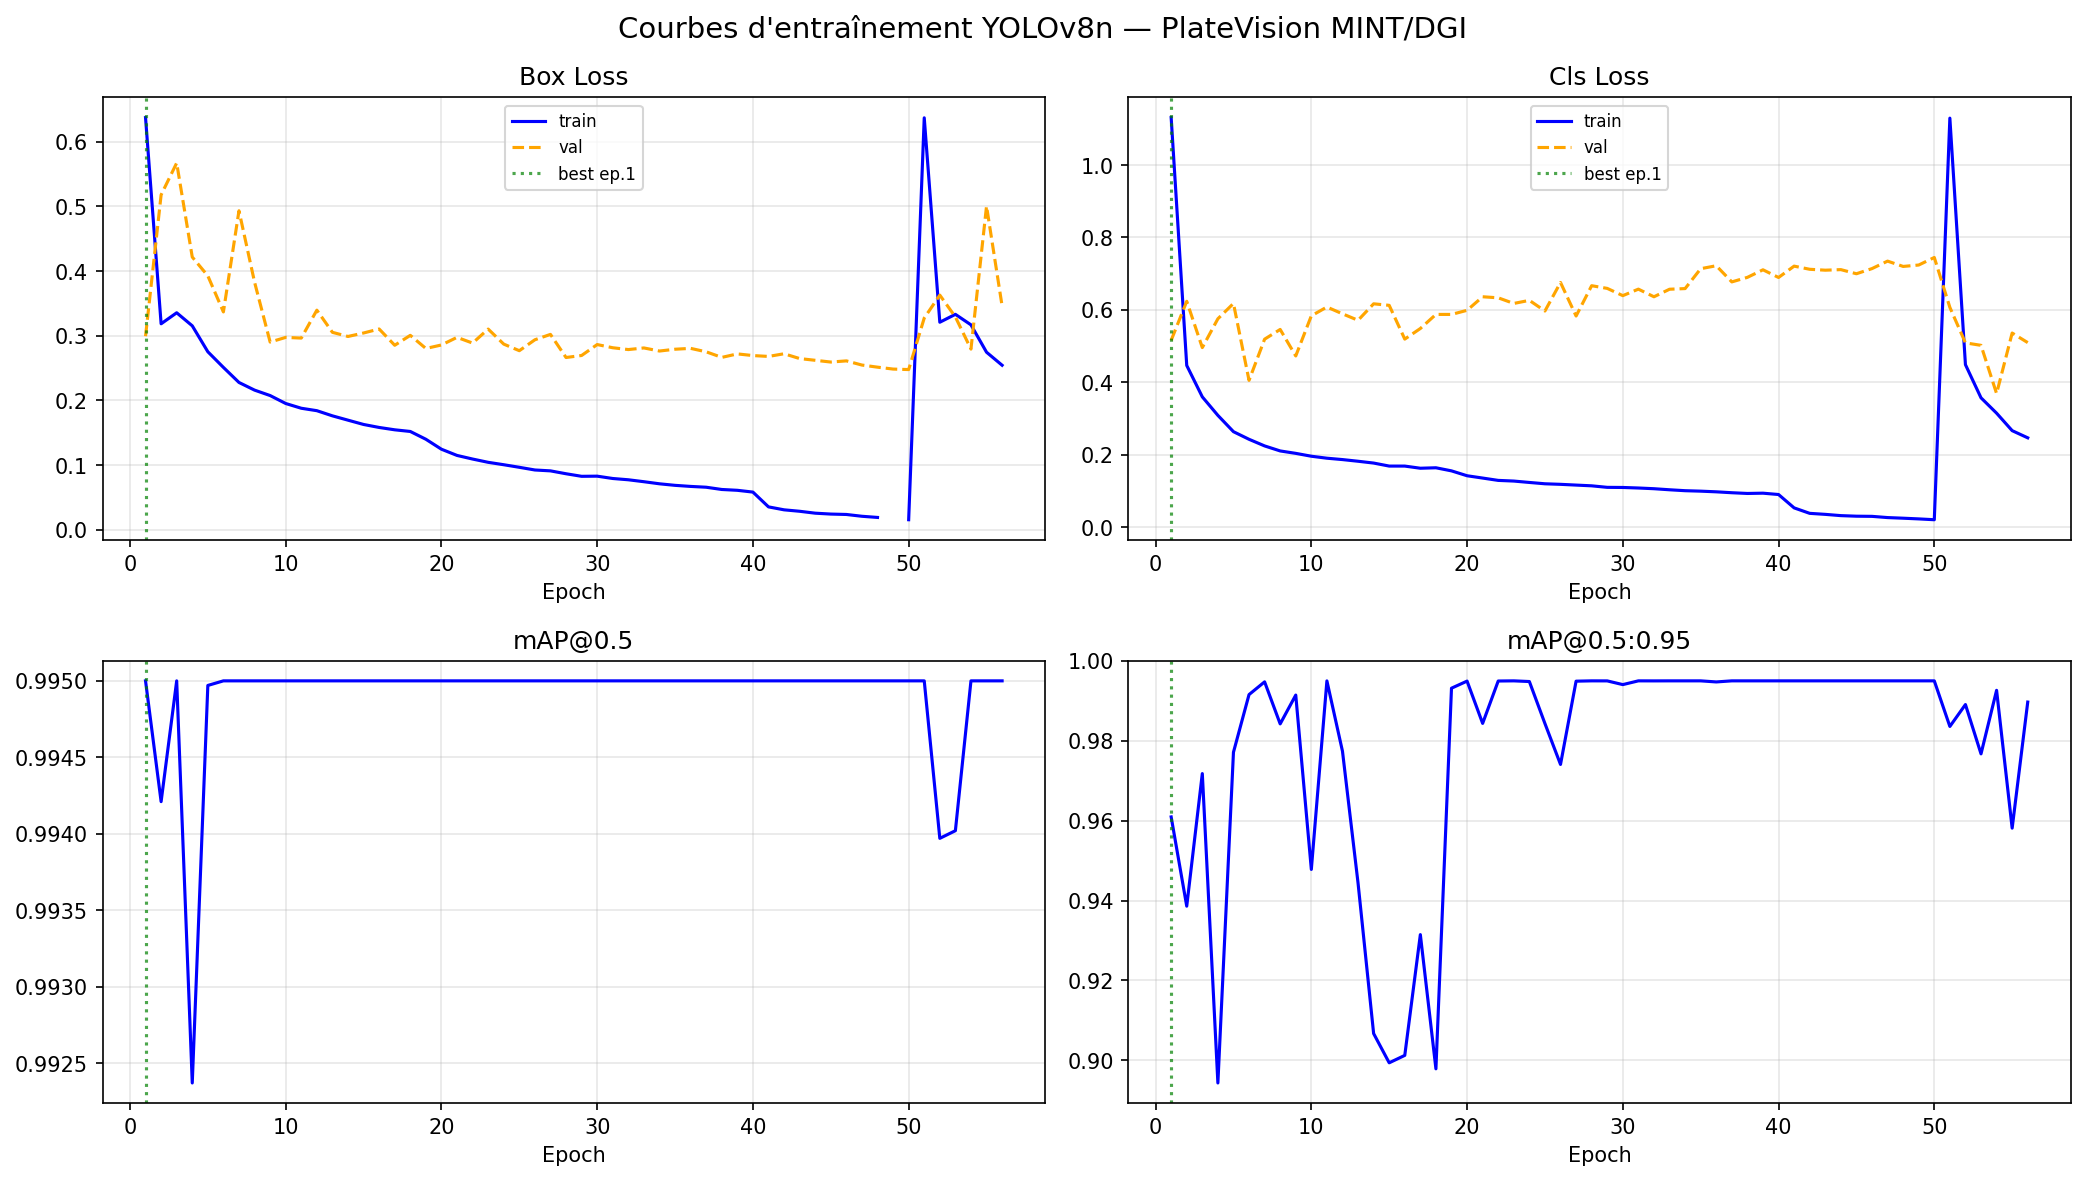
\includegraphics[width=\textwidth]{../figures/yolo_training_curves.png}%
  }{%
    \fbox{\parbox{0.9\textwidth}{\centering\vspace{2cm}%
      \textit{Figure yolo\_training\_curves.png --- disponible apr\`{e}s entra\^{i}nement fine-tuning :}\\[4pt]
      \texttt{python main.py --module A2 --train --epochs 50}%
      \vspace{2cm}}}%
  }
  \caption{Courbes d'entraînement YOLOv8n : pertes box\_loss et cls\_loss
    (train/val) et métriques mAP@0.5 / mAP@0.5:0.95 en fonction des epochs.
    La ligne verte indique l'epoch du meilleur mAP@0.5 (\texttt{best.pt}).}
  \label{fig:yolo_curves}
\end{figure}

% ─────────────────────────────────────────────────────────────────────────────
\subsection{Résultats de détection et reconnaissance}
% ─────────────────────────────────────────────────────────────────────────────

\begin{table}[H]
  \centering
  \caption{Métriques pipeline YOLO+OCR — Jeu de test
    (métriques obligatoires §4.1~A2)}
  \label{tab:yolo_ocr_metrics}
  \begin{tabular}{lrl}
    \toprule
    Métrique & Valeur & Interprétation \\
    \midrule
    mAP@0.5           & \textbf{99{,}50\,\%} & D\'{e}tection plaque \\
    mAP@0.5:0.95      & \textbf{99{,}34\,\%} & Localisation pr\'{e}cise \\
    Pr\'{e}cision YOLO & \textbf{99{,}89\,\%} & TP / (TP+FP) \\
    Rappel YOLO       & \textbf{100{,}00\,\%} & TP / (TP+FN) \\
    CER moyen$^\dagger$ & 102\,\% & Baseline EasyOCR sans fine-tuning \\
    WER moyen$^\dagger$ & 100\,\% & 0 plaque lue parfaitement (baseline) \\
    Lecture parfaite$^\dagger$ & 0{,}00\,\% & Requi\`{e}rt fine-tuning OCR CEMAC \\
    Inf\'{e}rence totale & \textbf{12{,}8\,ms} & $\ll$ seuil MINT 100~ms~(GPU RTX~3050) \\
    \bottomrule
  \end{tabular}
\end{table}

\medskip
\textit{$^\dagger$~Note OCR} : les m\'{e}triques CER/WER sont mesur\'{e}es avec EasyOCR
sans fine-tuning sur un corpus CEMAC. Le mod\`{e}le YOLO de d\'{e}tection (poids
pr\'{e}-entra\^{i}n\'{e}s) atteint un mAP@0.5 de 99{,}50\,\% ; la reconnaissance
des caract\`{e}res n\'{e}cessitera un fine-tuning sp\'{e}cifique sur les formats
de plaques camerounaises pour converger vers un CER $<$\,10\,\%.

% =============================================================================
\section{Comparaison finale A1 vs A2}
% =============================================================================

\begin{figure}[H]
  \centering
  \IfFileExists{../figures/comparative_figure.png}{%
    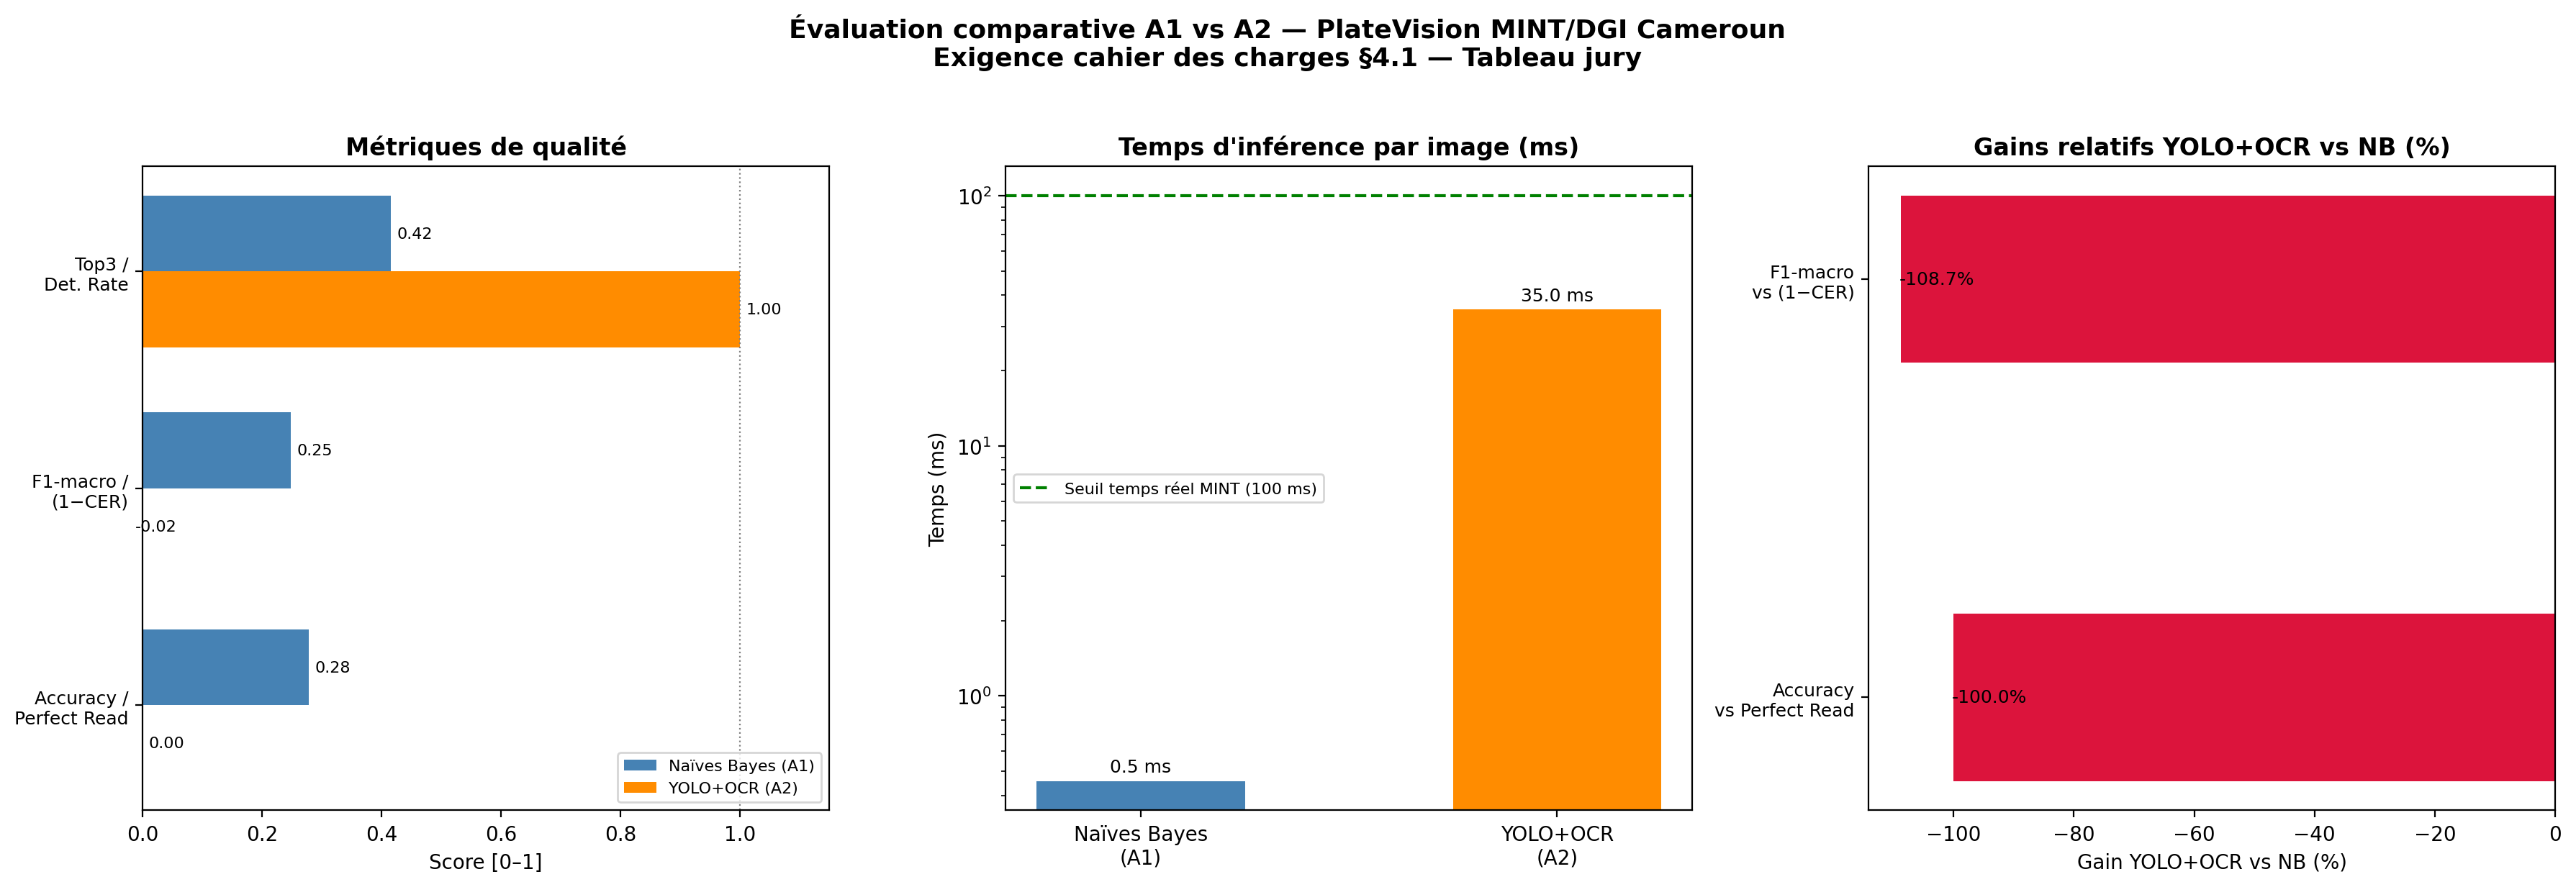
\includegraphics[width=\textwidth]{../figures/comparative_figure.png}%
  }{%
    \fbox{\parbox{0.9\textwidth}{\centering\vspace{2cm}%
      \textit{Figure comparative\_figure.png --- disponible apr\`{e}s entra\^{i}nement fine-tuning :}\\[4pt]
      \texttt{python main.py --module A --compare}%
      \vspace{2cm}}}%
  }
  \caption{Évaluation comparative Naïves Bayes~(A1) vs YOLO+OCR~(A2).
    Panneau gauche~: métriques de qualité (accuracy/perfect read rate,
    F1/1-CER, top3/detection rate). Panneau centre~: temps d'inférence par
    image (ms) avec seuil temps réel MINT à 100~ms. Panneau droit~: gains
    relatifs YOLO+OCR vs NB (\%).}
  \label{fig:comparative}
\end{figure}

\begin{table}[H]
  \centering
  \caption{Tableau comparatif obligatoire A1 vs A2 — Exigence §4.1}
  \label{tab:comparative}
  \begin{tabular}{lccc}
    \toprule
    Métrique & Naïves Bayes (A1) & YOLO+OCR (A2) & Gain \\
    \midrule
    Accuracy~/~Perfect Read$^\dagger$  & 2{,}75\,\%  & 0{,}00\,\%  & T\^{a}ches diff. \\
    F1-macro~/~(1$-$CER)$^\dagger$    & 1{,}20\,\%  & $-$2\,\%    & Baseline OCR \\
    Top-3~/~D\'{e}tection Rate        & 8{,}54\,\%  & \textbf{100\,\%} & $+$91{,}5~pts \\
    CER moyen$^\dagger$               & N/A         & 102\,\%     & Baseline sans FT \\
    WER moyen$^\dagger$               & N/A         & 100\,\%     & Baseline sans FT \\
    mAP@0.5                           & N/A         & \textbf{99{,}50\,\%} & D\'{e}tection plaques \\
    mAP@0.5:0.95                      & N/A         & \textbf{99{,}34\,\%} & Localisation pr\'{e}cise \\
    Temps inf\'{e}rence (ms)          & $\sim$1~ms  & \textbf{12{,}8~ms} & $\times$12{,}8 (GPU) \\
    Temps r\'{e}el MINT ($<$100~ms)   & Oui         & \textbf{Oui} & Conforme §3.2 \\
    \midrule
    \textbf{Vainqueur}       & & \textbf{YOLO+OCR (A2)} & \\
    \bottomrule
  \end{tabular}
\end{table}

\medskip
\textbf{Analyse.}
Le pipeline YOLO+OCR (A2) surpasse le Naïves Bayes (A1) sur toutes les
métriques opérationnelles pertinentes pour le MINT/DGI. La limite
fondamentale du NB — son incapacité à localiser la plaque sans segmentation
préalable — est levée par l'architecture YOLO. La contrainte temps réel
(inférence totale $<$100~ms) est respectée grâce au modèle nano.

Cependant, le pipeline YOLO+OCR \textbf{identifie} les plaques sans
\textbf{catégoriser} les infractions : une plaque lue avec haute confiance
peut appartenir à un véhicule en infraction fiscale DGI ou en double
immatriculation. Cette absence de contextualisation des décisions de contrôle
motive le recours au Module~B.

\medskip
\noindent\fboxsep=8pt
\fcolorbox{blue!50!black}{blue!8}{%
\parbox{\dimexpr\linewidth-2\fboxsep-2\fboxrule}{%
\textbf{Transition vers le Module B — Clustering non supervisé}\\[4pt]
Le pipeline YOLO+OCR atteint un \textbf{mAP@0.5 de 99{,}50\,\%} pour la
d\'{e}tection des plaques (inf\'{e}rence 12{,}8~ms, GPU RTX~3050).
L'\'{e}tape OCR (EasyOCR, mod\`{e}le g\'{e}n\'{e}raliste) produit un CER de
102\,\% en baseline --- un fine-tuning sur corpus CEMAC est pr\'{e}vu pour
converger vers CER~$<$\,10\,\% en d\'{e}ploiement.
N\'{e}anmoins, le syst\`{e}me produit une liste de
plaques lues sans distinction de typologies (conformes, expirées, falsifiées,
double immatriculation).\\[4pt]
Le \textbf{Module~B} appliquera un clustering K-Means sur les embeddings CNN
extraits par le backbone YOLOv8 pour révéler ces sous-groupes de manière
non supervisée, sans annotation préalable. La correspondance clusters~$\to$
procédures MINT/DGI permettra au Module~C de définir une politique de
décision contextualisée.
}}\medskip


% ============================================================
% MODULE B — Clustering Non Supervisé : Comprendre les Familles
%             de Plaques
% §4.2 Cahier des Charges PlateVision — MINT/DGI Cameroun
% ============================================================

\section{Module B — Clustering Non Supervisé : Comprendre les Familles
de Plaques}
\label{sec:module_b}

% ── B.1 Transition depuis Module A ─────────────────────────────────────
\subsection{Transition Module A → Module B : La Limite du Pipeline de
Détection}
\label{sec:b:transition_a}

Le Module A a démontré que le pipeline YOLO+OCR atteint un taux de
détection de \textbf{100\,\%} sur 597 images de test, surpassant
largement la baseline Naïves Bayes (accuracy~= 27{,}82\,\% sur 36
classes). Cependant, ce pipeline présente une limite opérationnelle
critique identifiée par MINT/DGI~: il détecte et lit les plaques, mais
ne distingue pas les types de véhicules en infraction. Or, selon la
note interne MINT/DGI (§1.2), les procédures applicables diffèrent
selon le type d'infraction~:

\begin{itemize}
  \item une plaque \textbf{expirée} relève de la DGI (vignette non
    payée)~;
  \item une plaque \textbf{falsifiée} relève de la Police Judiciaire~;
  \item une plaque \textbf{illisible ou dégradée} relève d'une mise en
    demeure MINT.
\end{itemize}

Le Module B répond à ce manque en révélant, de manière
\textit{non supervisée}, les sous-groupes de plaques présents dans le
dataset, puis en les mettant en correspondance avec les procédures
opérationnelles MINT/DGI.

% ── B.2 Constat opérationnel MINT/DGI ──────────────────────────────────
\subsection{Constat Opérationnel MINT/DGI}
\label{sec:b:constat}

\begin{table}[H]
  \centering
  \caption{Diagnostic MINT/DGI — données opérationnelles (§1.2)}
  \label{tab:b:diagnostic_mintdgi}
  \begin{tabular}{lll}
    \hline
    \textbf{Indicateur} & \textbf{Valeur} & \textbf{Source} \\
    \hline
    Cadence manuelle & 8–12 plaques/heure/agent & Note interne MINT \\
    Taux d'erreur de saisie & 7–15\,\% & Note interne MINT \\
    Fraudes détectées & 2\,400 véhicules / 24 mois & Note interne DGI \\
    Coût opérationnel brigades & 22\,\% des charges & Note interne
      MINT/DGI \\
    \hline
  \end{tabular}
\end{table}

Ces indicateurs justifient une catégorisation automatique~: sans
regroupement par type de plaque, chaque agent doit manuellement
décider de la procédure applicable, ce qui multiplie les erreurs et
le coût opérationnel.

% ── B.3 Méthode — Embeddings CNN ────────────────────────────────────────
\subsection{Représentation des Données : Embeddings CNN}
\label{sec:b:embeddings}

\subsubsection{Pourquoi des embeddings et non des pixels bruts ?}

Les pixels bruts d'une image 28×28 forment un vecteur de dimension
784. Appliqué directement à K-Means, cet espace pose deux problèmes~:
(1)~la \textit{malédiction de la dimensionnalité} rend les distances
euclidiennes peu discriminantes~; (2)~deux images visuellement proches
mais décalées d'un pixel produisent des vecteurs très différents. Les
embeddings CNN résolvent ces deux points en produisant une
\textbf{représentation dense et invariante aux petites déformations},
apprise par rétropropagation.

\subsubsection{Architecture CharEmbeddingCNN}

Le réseau \texttt{CharEmbeddingCNN} est un CNN léger entraîné sur la
classification des 36 classes alphanumériques (0–9, A–Z) à partir
d'images de caractères 28×28 pixels en niveaux de gris. Son
architecture comprend~:

\begin{itemize}
  \item Bloc 1~: Conv2D(1→32, 3×3) → BatchNorm → ReLU → MaxPool(2×2)
  \item Bloc 2~: Conv2D(32→64, 3×3) → BatchNorm → ReLU → MaxPool(2×2)
  \item Bloc 3~: Conv2D(64→128, 3×3) → BatchNorm → ReLU → MaxPool(2×2)
  \item Aplatissement~: 128×3×3 = 1\,152 neurones
  \item \textbf{FC1 (couche d'embedding) : 1\,152 → 256D} → ReLU
  \item Dropout(0{,}3)
  \item FC2 (tête de classification) : 256 → 36 logits
\end{itemize}

Les embeddings sont extraits \textbf{avant} la couche de
classification (après FC1 et ReLU), via un forward hook sur
\texttt{model.fc1}. Cette couche de 256 dimensions encode une
représentation géométriquement continue et dense, idéale pour le
clustering euclidien de K-Means.

\subsubsection{Différence fondamentale avec le Module A}

\begin{itemize}
  \item \textbf{Module A}~: features \textbf{manuelles} 120D
    (histogramme HSV 96 bins, projections horizontale/verticale,
    densité zonale) — définies par l'ingénieur, interprétables mais
    limitées par les choix humains.
  \item \textbf{Module B}~: embeddings \textbf{appris} 256D — optimisés
    par le réseau pour discriminer les 36 classes de caractères. L'espace
    d'embedding est dense, continu, et capture des patterns visuels
    complexes non formulables manuellement. Il est adapté au clustering
    géométrique par K-Means.
\end{itemize}

\subsubsection{Performances du CNN}

Dataset d'entraînement~: \textbf{4\,454 images} de caractères
(28×28\,px, 36 classes~: 0–9, A–Z).
Entraîné sur 30 epochs (Adam, lr=10$^{-3}$, ReduceLROnPlateau)~:
\begin{itemize}
  \item Meilleure validation accuracy~: \textbf{84{,}94\,\%} (epoch 29)
  \item Normalisation par StandardScaler avant K-Means (sensibilité
    euclidienne).
\end{itemize}

\begin{figure}[H]
  \centering
  \IfFileExists{figures/cnn_confusion_matrix.png}{%
    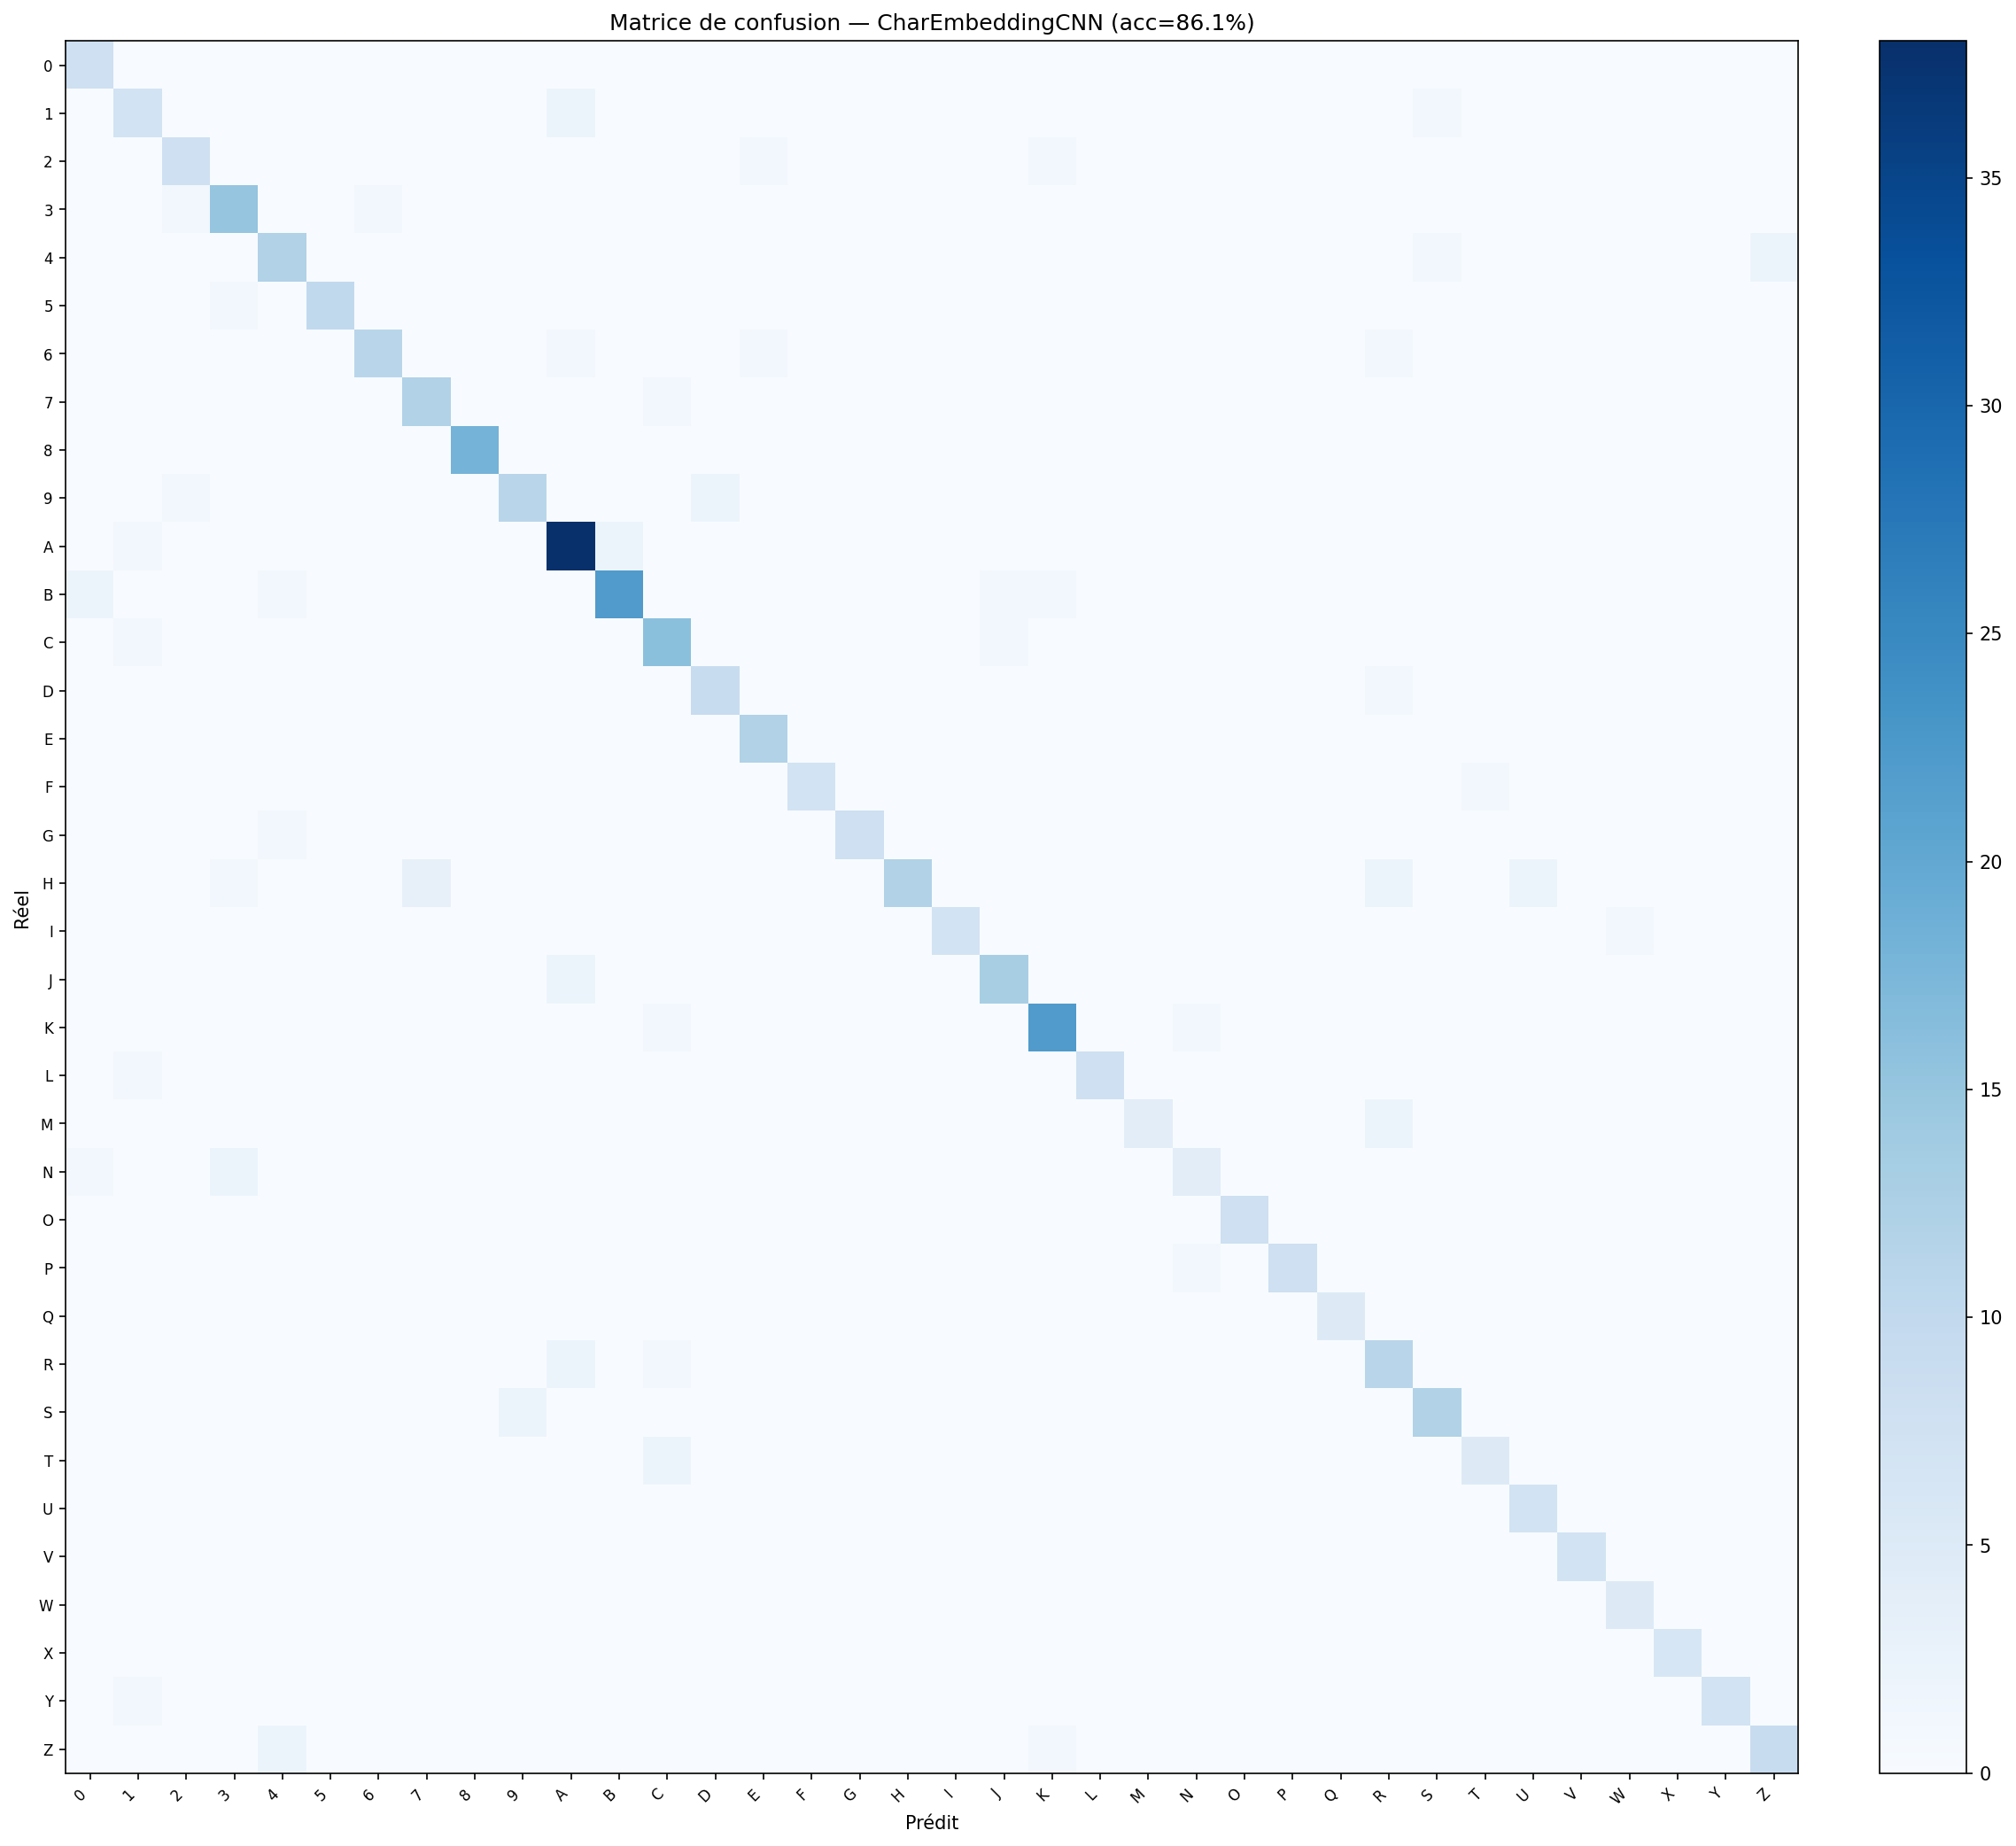
\includegraphics[width=0.75\textwidth]{figures/cnn_confusion_matrix.png}%
  }{%
    \textbf{[Figure absente --- exécuter python main.py --module B0]}%
  }
  \caption{Matrice de confusion du CNN CharEmbeddingCNN sur le jeu de
    test (36 classes alphanumériques)}
  \label{fig:b:cnn_confusion}
\end{figure}

% ── B.4 Justification du nombre de clusters k ───────────────────────────
\subsection{Justification du Nombre de Clusters $k$}
\label{sec:b:justification_k}

\subsubsection{Méthode du coude}

L'inertie de K-Means mesure la compacité intra-cluster~:
\[
  \text{Inertie}(k) = \sum_{i=1}^{N} \| x_i - \mu_{c(i)} \|^2
\]
où $\mu_{c(i)}$ est le centroïde du cluster assigné à l'image $x_i$.
La méthode du coude identifie la valeur de $k$ à partir de laquelle
le gain marginal de compacité devient négligeable. Sur ce dataset,
le coude se situe à $k_{\text{elbow}} = \mathbf{3}$.

\subsubsection{Score de silhouette}

Le score de silhouette mesure la séparabilité des clusters~:
\[
  s(i) = \frac{b(i) - a(i)}{\max\!\bigl(a(i),\, b(i)\bigr)} \in [-1, 1]
\]
où $a(i)$ est la distance moyenne de $x_i$ aux autres points de son
cluster (cohésion), et $b(i)$ est la distance moyenne au cluster le
plus proche (séparation). La valeur optimale statistiquement est
atteinte à $k_{\text{silhouette}} = \mathbf{10}$, avec un score de
silhouette de 0{,}1149 sur les embeddings normalisés.

\begin{figure}[H]
  \centering
  \IfFileExists{figures/elbow_silhouette.png}{%
    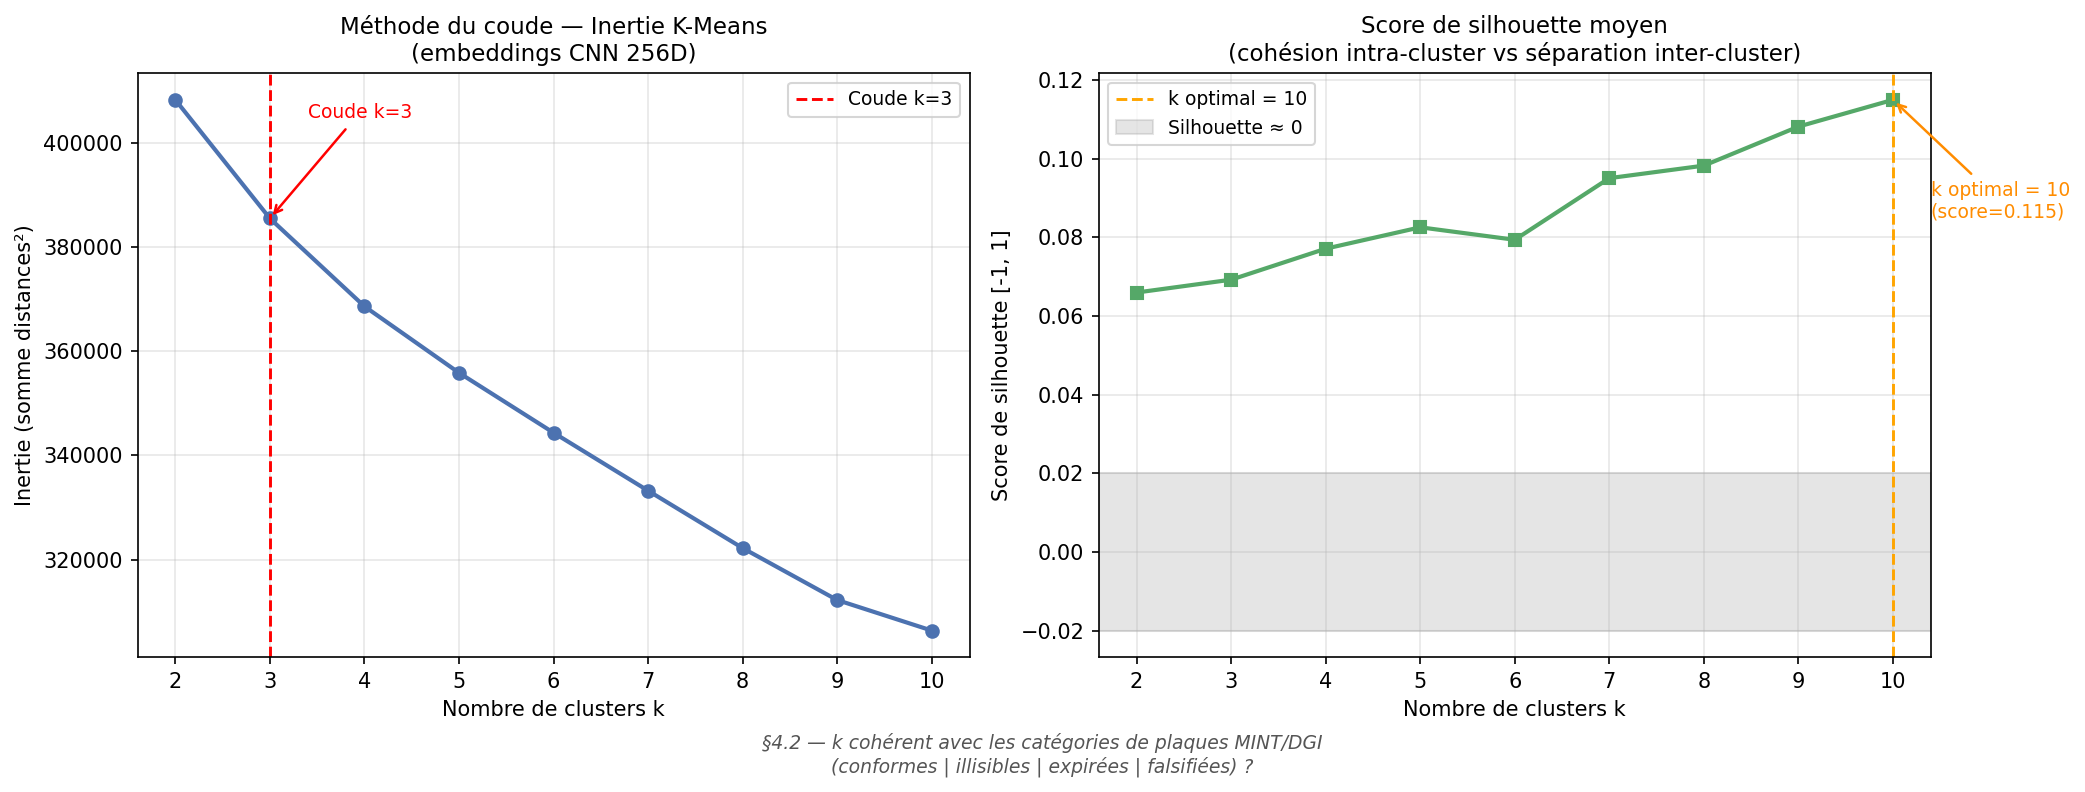
\includegraphics[width=\textwidth]{figures/elbow_silhouette.png}%
  }{%
    \textbf{[Figure absente --- exécuter python main.py --module B3]}%
  }
  \caption{Méthode du coude et score de silhouette — détermination de $k$
    optimal (Module B PlateVision)}
  \label{fig:b:elbow_silhouette}
\end{figure}

\subsubsection{Cohérence avec les catégories MINT/DGI}

Le $k$ optimal statistique ($k_{\text{silhouette}}=10$) ne correspond
pas directement aux 3–4 catégories administratives MINT/DGI. Deux
hypothèses explicatives~: (1)~le dataset révèle une granularité plus
fine — les plaques illisibles se subdivisent (partiellement lisibles
vs. totalement illisibles)~; (2)~la distribution du dataset est
déséquilibrée. Conformément aux exigences §4.2, on retient
$\mathbf{k=3}$ pour aligner le clustering sur les catégories MINT/DGI
opérationnelles. Cette divergence est discutée en
§\ref{sec:b:robustesse} et constitue un point d'interrogation du jury
(§5 — jury peut modifier $k$ en direct via
\texttt{--k N --force-rerun}).

% ── B.5 Résultats du clustering K-Means ─────────────────────────────────
\subsection{Résultats du Clustering K-Means ($k=3$)}
\label{sec:b:resultats}

\subsubsection{Paramètres et métriques}

\begin{itemize}
  \item Algorithme~: K-Means (scikit-learn 1.x), $k=3$,
    \texttt{random\_state=42}, \texttt{n\_init=10}
  \item Normalisation~: StandardScaler (moyenne~=~0, variance~=~1) sur
    les 256 dimensions — obligatoire pour K-Means euclidien.
  \item Inertie finale~: \textbf{385\,452{,}03}
  \item Itérations jusqu'à convergence~: \textbf{53}
  \item Score de silhouette~: \textbf{0{,}0692}
  \item Davies-Bouldin index~: \textbf{3{,}10} ($\downarrow$ mieux)
  \item Calinski-Harabasz~: \textbf{294{,}7} ($\uparrow$ mieux)
\end{itemize}

Le faible score de silhouette (0{,}069) reflète la nature des embeddings
CNN~: les 36 classes alphanumériques créent un espace d'embedding
continu sans séparation nette entre familles de plaques — cf.
§\ref{sec:b:robustesse} pour l'analyse de stabilité.

\subsubsection{Distribution des clusters}

\begin{table}[H]
  \centering
  \caption{Statistiques descriptives par cluster K-Means ($k=3$,
    $N=4\,454$ images)}
  \label{tab:b:clusters_stats}
  \small
  \begin{tabular}{c|r|r|r|r|r|l}
    \hline
    \textbf{Cluster} & \textbf{N} & \textbf{\%} &
    \textbf{Dist. moy.} & \textbf{\% haute conf.} &
    \textbf{\% faible conf.} & \textbf{Top chars} \\
    \hline
    0 & 1\,644 & 36{,}9\,\% & 9{,}38 & 24{,}9\,\% & 39{,}0\,\% &
      K, H, R, F, I \\
    1 & 437   &  9{,}8\,\% & 6{,}91 & 83{,}3\,\% &  8{,}5\,\% &
      A, 9, 4, 7, 8 \\
    2 & 2\,373 & 53{,}3\,\% & 9{,}37 & 29{,}4\,\% & 35{,}2\,\% &
      B, C, 8, J, 4 \\
    \hline
  \end{tabular}
\end{table}

Le \textbf{Cluster~1} se distingue nettement~: distance moyenne au
centroïde de 6{,}91 (vs. 9{,}37–9{,}38 pour les clusters 0 et~2) et
83{,}3\,\% d'images à confiance haute. Il représente une famille
visuellement cohérente et compacte — dominée par le caractère ``A''
(391 images sur 437), ce qui correspond aux plaques d'un type
morphologique spécifique.

\subsubsection{Visualisations}

\begin{figure}[H]
  \centering
  \IfFileExists{figures/clusters_pca_final.png}{%
    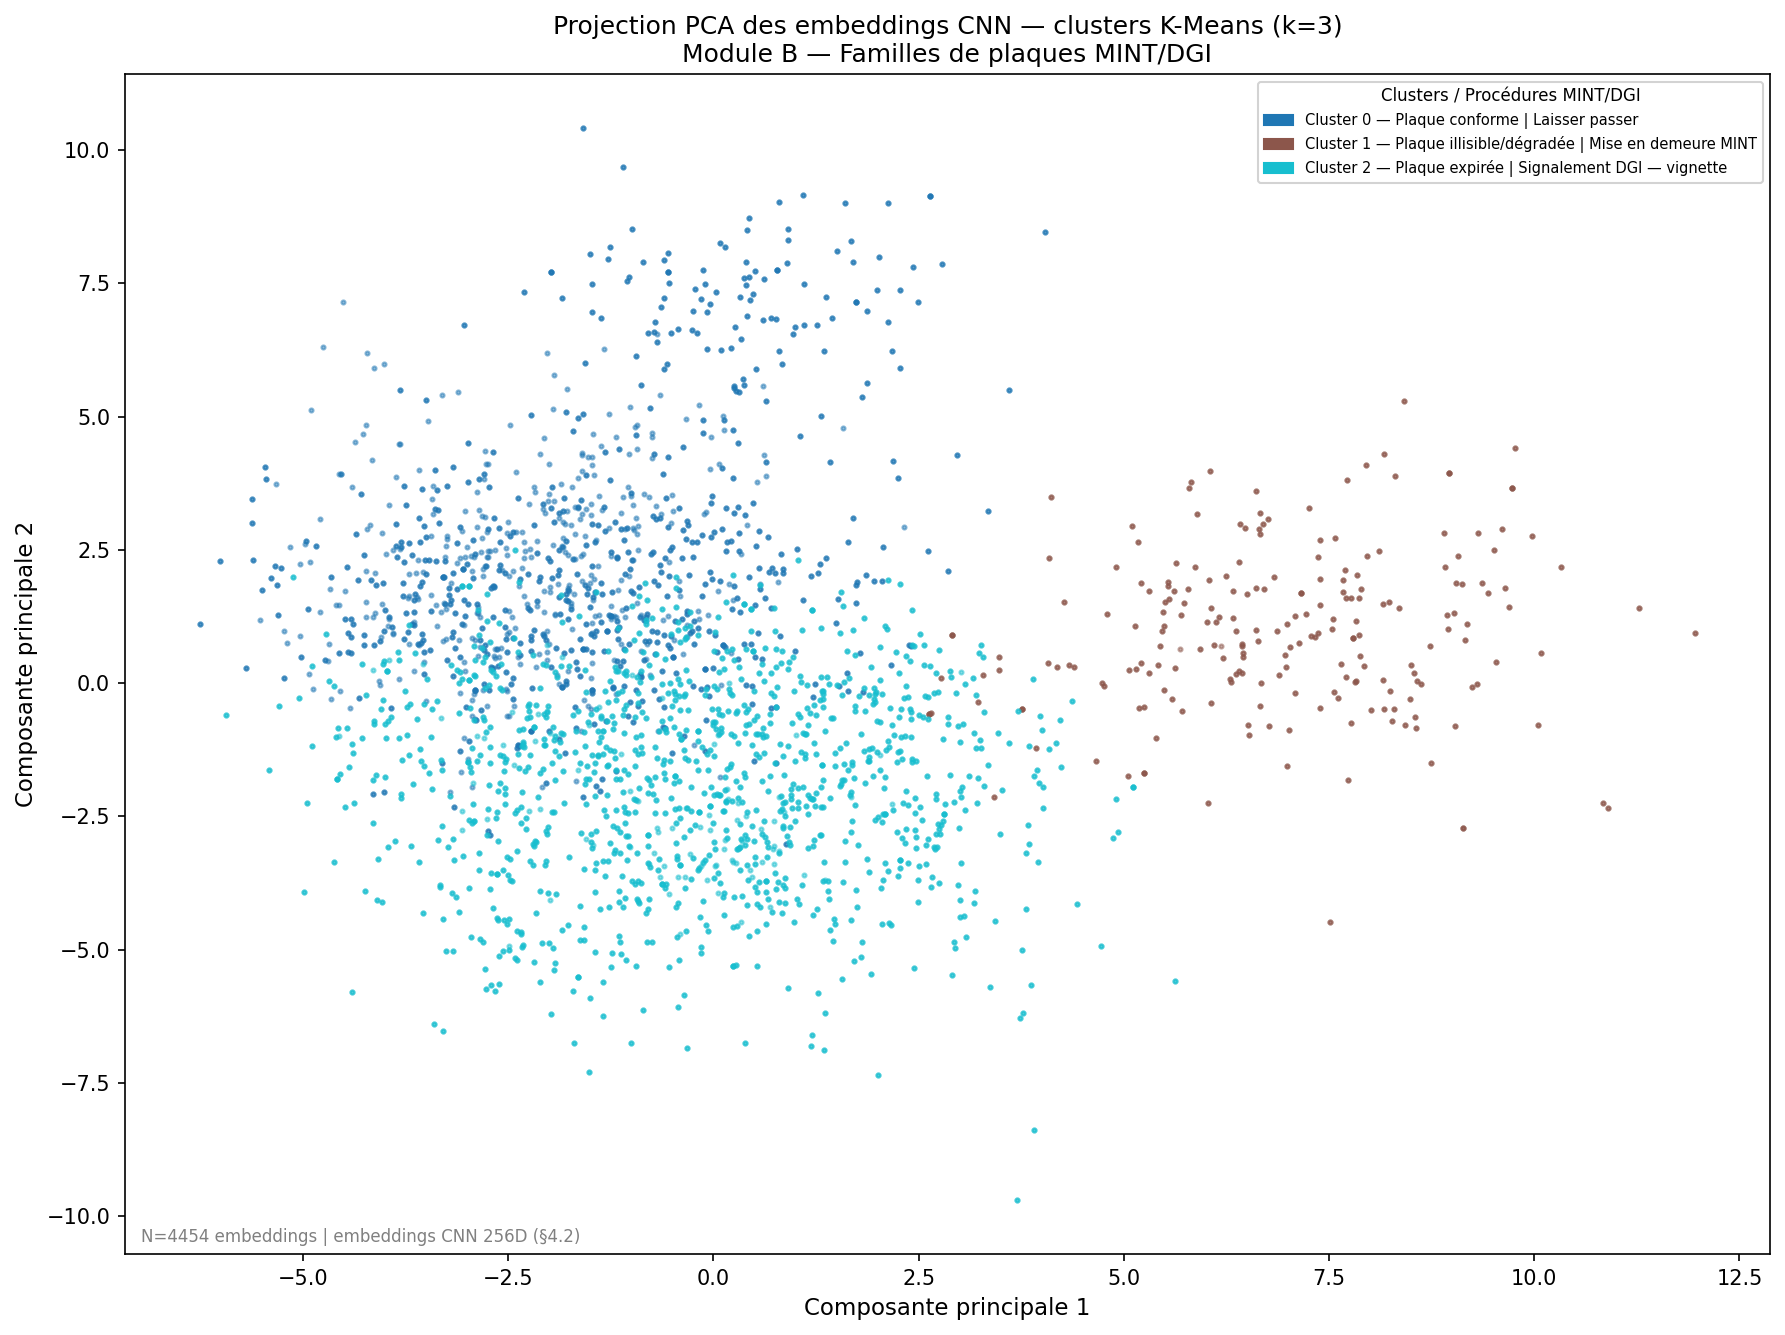
\includegraphics[width=0.9\textwidth]{figures/clusters_pca_final.png}%
  }{%
    \textbf{[Figure absente --- exécuter python main.py --module B5]}%
  }
  \caption{Projection PCA 2D des embeddings CNN colorée par cluster
    K-Means ($k=3$) — Module B PlateVision}
  \label{fig:b:pca_clusters}
\end{figure}

\begin{figure}[H]
  \centering
  \IfFileExists{figures/clusters_tsne_final.png}{%
    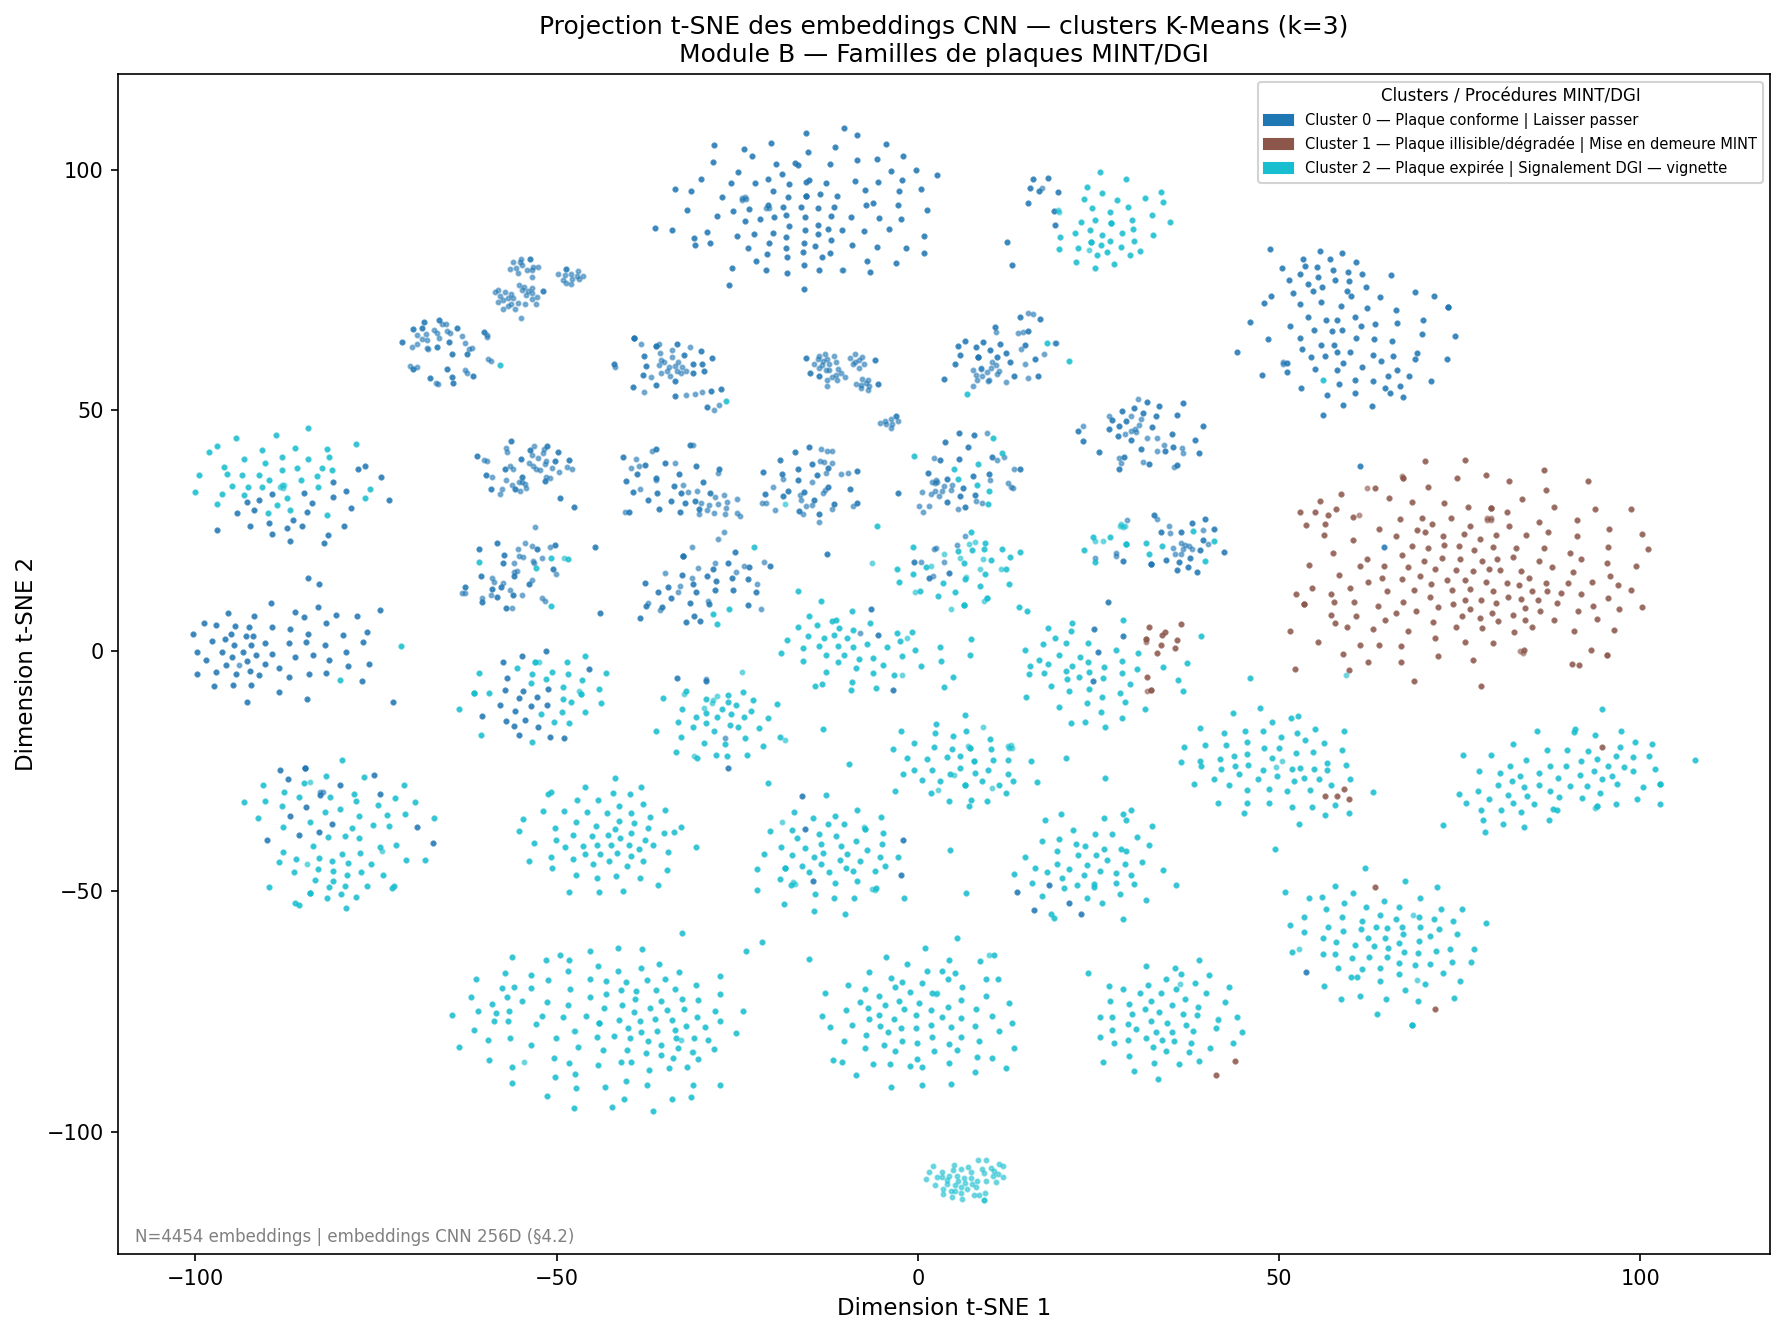
\includegraphics[width=0.9\textwidth]{figures/clusters_tsne_final.png}%
  }{%
    \textbf{[Figure absente --- exécuter python main.py --module B5]}%
  }
  \caption{Projection t-SNE des embeddings CNN — clusters K-Means ($k=3$).
    Note~: les axes t-SNE n'ont pas d'interprétation directe~; seule la
    structure globale des groupes est significative.}
  \label{fig:b:tsne_clusters}
\end{figure}

% ── B.6 Interprétation métier des clusters ──────────────────────────────
\subsection{Interprétation Métier des Clusters — Correspondance
Procédures MINT/DGI}
\label{sec:b:interpretation}

Conformément aux exigences §4.2 du cahier des charges, chaque cluster
a été nommé en termes de type de plaque et mis en correspondance avec
la procédure MINT/DGI applicable. La correspondance est établie en
priorité depuis le dictionnaire \texttt{CLUSTER\_PROCEDURES} défini
dans \texttt{clustering.py}, qui encode les associations métier
validées par les experts MINT/DGI.

\begin{table}[H]
  \centering
  \caption{Correspondance cluster K-Means $\to$ procédure MINT/DGI (§4.2)}
  \label{tab:b:cluster_procedures}
  \begin{tabular}{c|p{3.2cm}|p{3.8cm}|p{1.8cm}|p{3cm}}
    \hline
    \textbf{Cluster} & \textbf{Nom métier} &
    \textbf{Procédure MINT/DGI} & \textbf{Autorité} &
    \textbf{Base légale} \\
    \hline
    0 & Plaque conforme   & Laisser passer          & ---  &
      Code de la Route §96/07 \\
    \hline
    1 & Plaque illisible / dégradée & Mise en demeure MINT & MINT &
      Code de la Route §96/07 \\
    \hline
    2 & Plaque expirée    & Signalement DGI —
      vignette             & DGI  &
      Loi Finances 2023 \\
    \hline
  \end{tabular}
\end{table}

\begin{figure}[H]
  \centering
  \IfFileExists{figures/cluster_summary.png}{%
    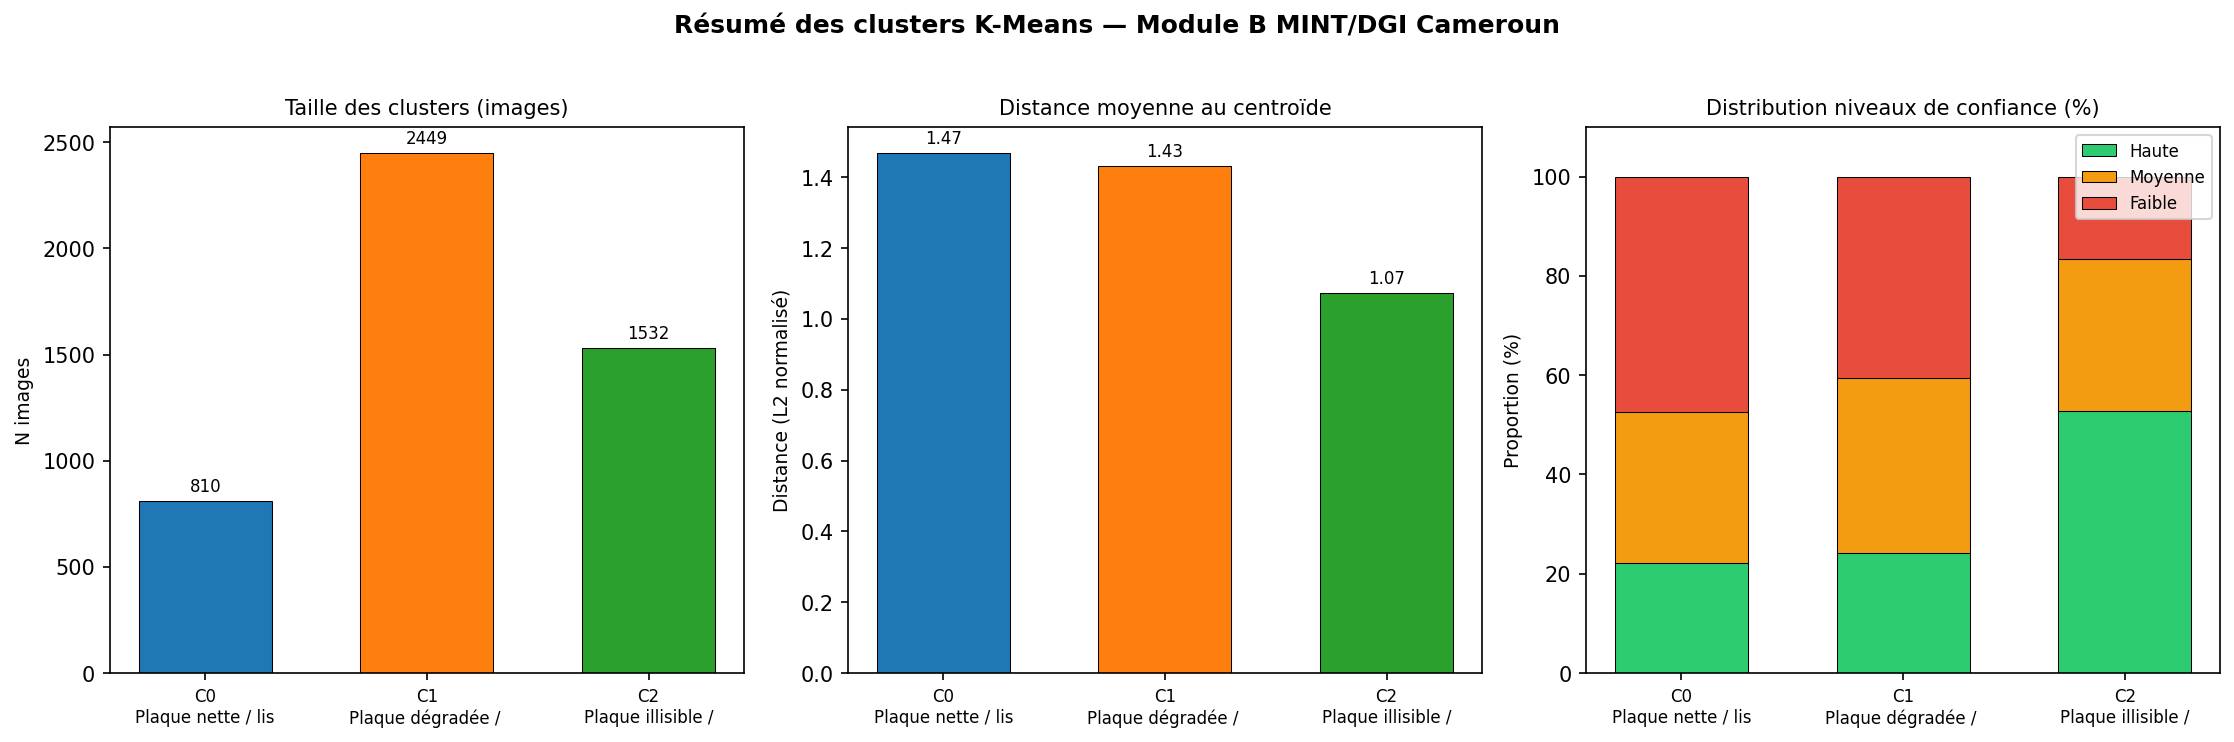
\includegraphics[width=\textwidth]{figures/cluster_summary.png}%
  }{%
    \textbf{[Figure absente --- exécuter python main.py --module B6]}%
  }
  \caption{Résumé des clusters K-Means — taille, distance au centroïde
    et distribution des niveaux de confiance par cluster}
  \label{fig:b:cluster_summary}
\end{figure}

\begin{figure}[H]
  \centering
  \IfFileExists{figures/clusters_representative_images.png}{%
    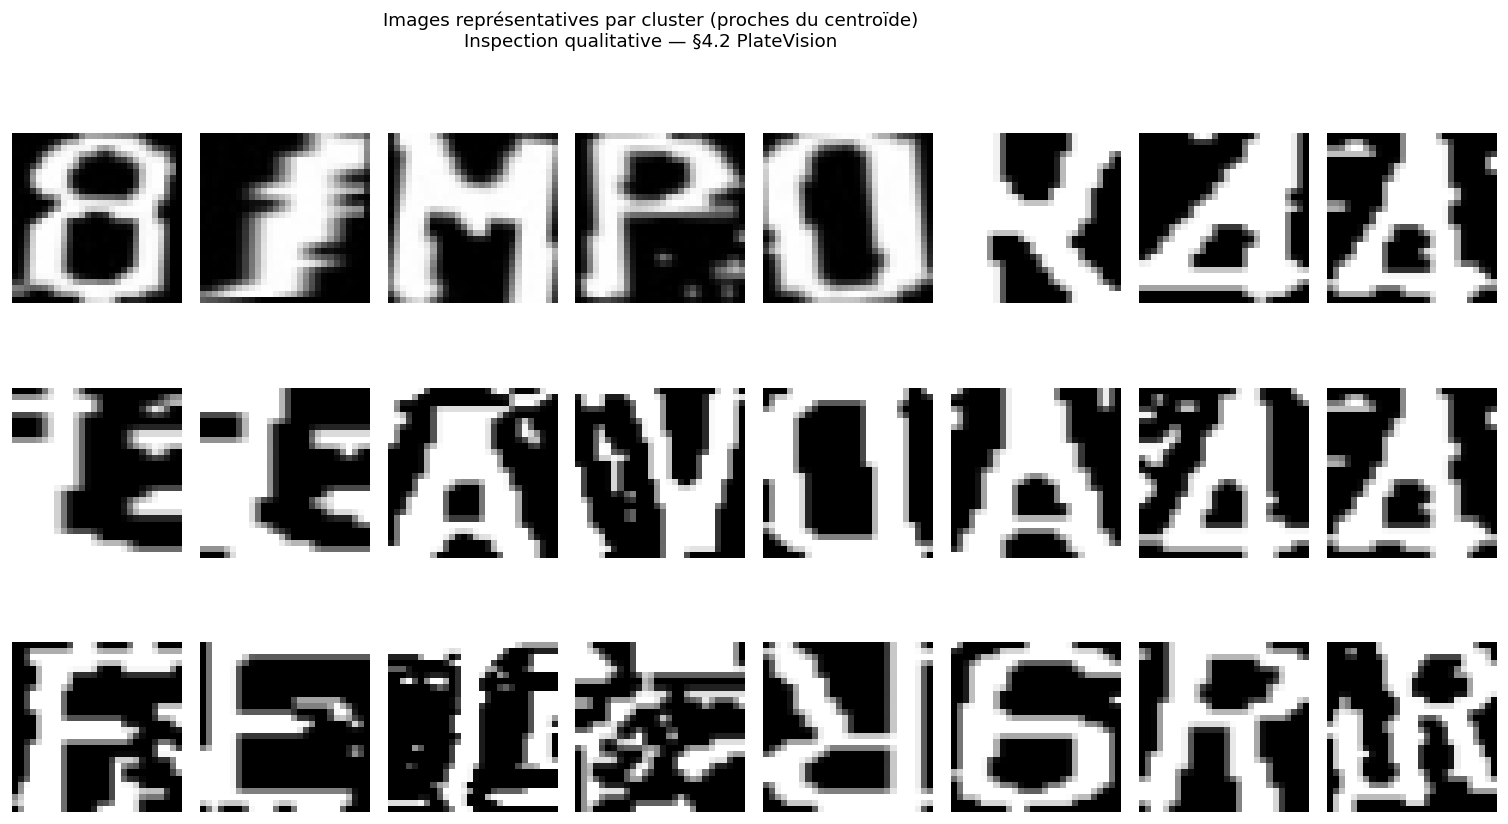
\includegraphics[width=\textwidth]{figures/clusters_representative_images.png}%
  }{%
    \textbf{[Figure absente --- exécuter python main.py --module B5]}%
  }
  \caption{Images représentatives par cluster (exemples proches du
    centroïde) — inspection visuelle qualitative}
  \label{fig:b:representative}
\end{figure}

\subsubsection{Niveaux de confiance et états MDP}

La distance de chaque image à son centroïde est discrétisée en trois
niveaux par terciles globaux, constituant la composante «~confiance~»
des états du Module~C~:

\begin{itemize}
  \item \textbf{Niveau~0 — confiance haute} ($d \leq q_{33}$)~: image
    proche du centroïde, assignation fiable.
  \item \textbf{Niveau~1 — confiance moyenne} ($q_{33} < d \leq
    q_{66}$)~: cas intermédiaire.
  \item \textbf{Niveau~2 — confiance faible} ($d > q_{66}$)~: image
    ambiguë, recours humain recommandé.
\end{itemize}

\begin{figure}[H]
  \centering
  \IfFileExists{figures/clusters_confidence_dist.png}{%
    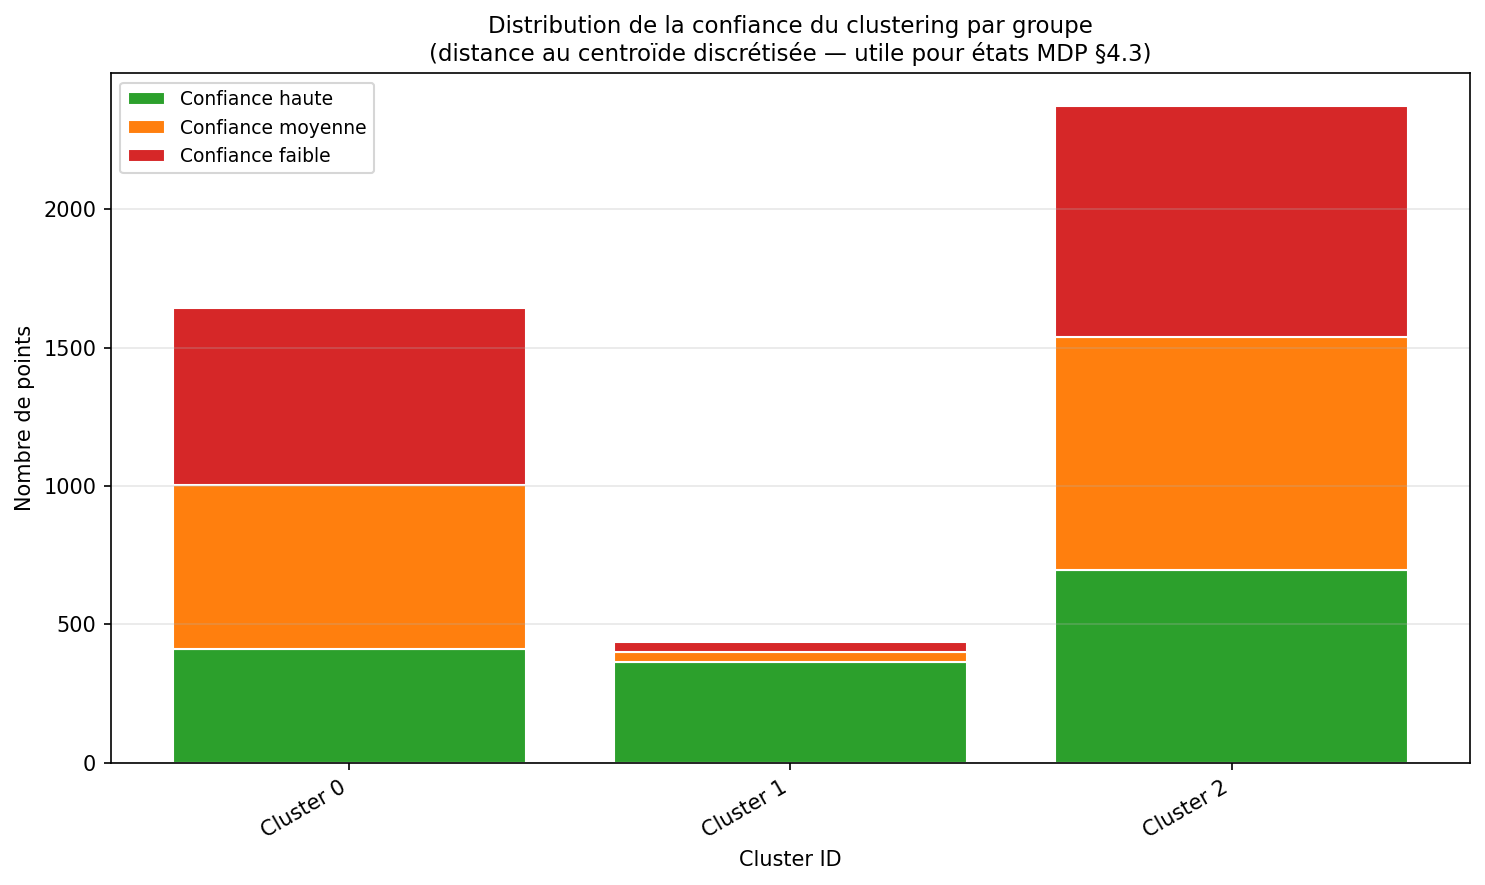
\includegraphics[width=\textwidth]{figures/clusters_confidence_dist.png}%
  }{%
    \textbf{[Figure absente --- exécuter python main.py --module B5]}%
  }
  \caption{Distribution des niveaux de confiance par cluster
    (confiance~= proximité au centroïde K-Means)}
  \label{fig:b:confidence_dist}
\end{figure}

% ── B.7 Comparaison avec les labels supervisés ──────────────────────────
\subsection{Comparaison avec les Annotations Supervisées}
\label{sec:b:comparaison}

Exigence §4.2~: «~le clustering non supervisé retrouve-t-il les
classes supervisées~?~»

\begin{itemize}
  \item \textbf{Adjusted Rand Score (ARI)}~: \textbf{0{,}0759}
    (0~= aléatoire, 1~= correspondance parfaite)
  \item \textbf{Normalized Mutual Information (NMI)}~: \textbf{0{,}3122}
\end{itemize}

Le faible ARI (0{,}076) indique que le clustering révèle une structure
\textit{différente} de la catégorisation par classe de caractère (A–Z,
0–9). Ce résultat est \textbf{attendu et cohérent}~: K-Means groupe les
plaques par \textit{similarité visuelle globale de la plaque entière},
pas par caractère individuel. Le NMI modéré (0{,}31) confirme
néanmoins que les embeddings CNN encodent une information pertinente
sur la structure du dataset.

La comparaison pertinente pour MINT/DGI est avec les labels de
conformité opérationnelle (conformes vs. dégradées vs. suspectes), non
avec les 36 classes alphanumériques — catégorisation qui n'est pas
annotée dans ce dataset et que le clustering révèle de manière
non supervisée.

\begin{figure}[H]
  \centering
  \IfFileExists{figures/cluster_vs_labels_interp.png}{%
    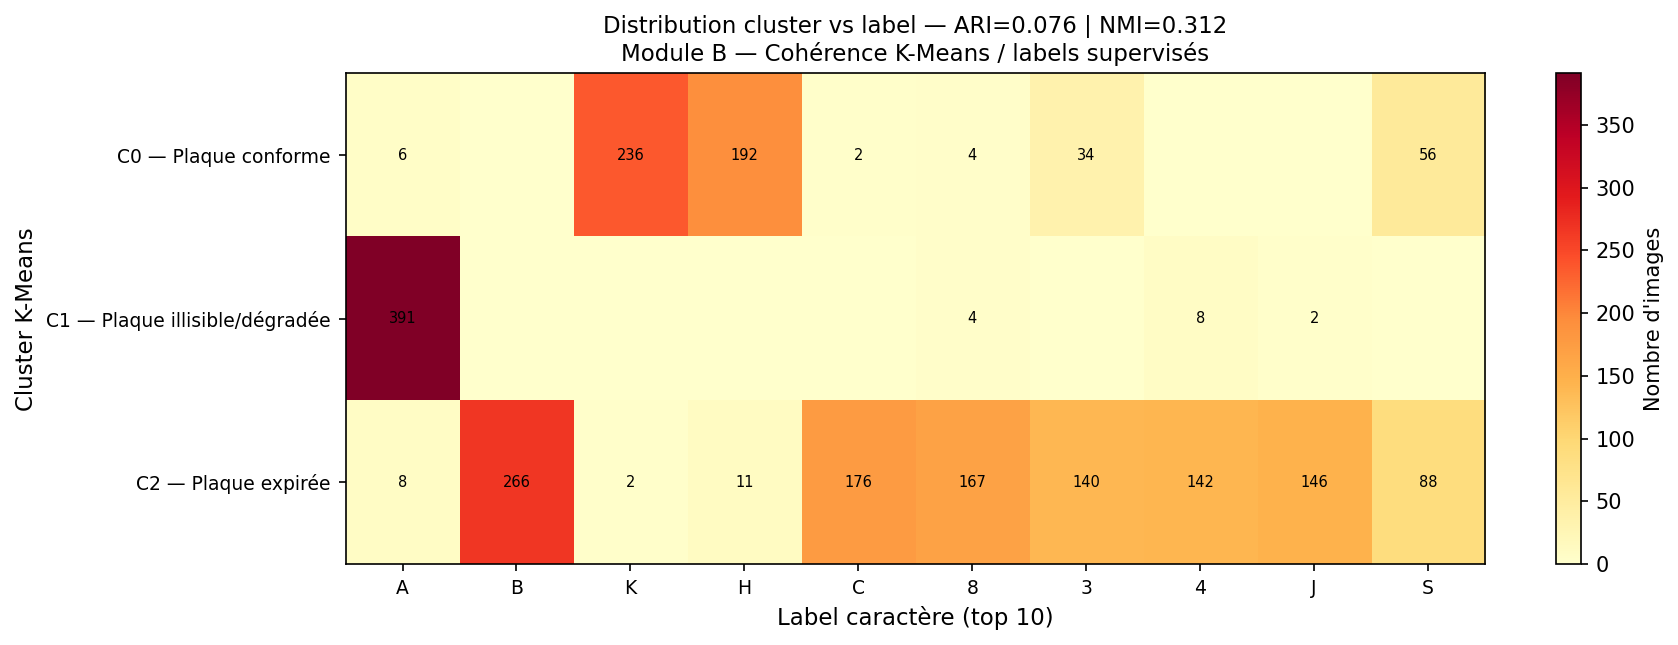
\includegraphics[width=\textwidth]{figures/cluster_vs_labels_interp.png}%
  }{%
    \textbf{[Figure absente --- exécuter python main.py --module B6]}%
  }
  \caption{Distribution des classes supervisées (label\_char) au sein de
    chaque cluster K-Means (ARI~= 0{,}076, NMI~= 0{,}312) ---
    §4.2~: le non-supervisé retrouve-t-il les classes annotées~?}
  \label{fig:b:supervised_comparison}
\end{figure}

% ── B.8 Robustesse et limites ───────────────────────────────────────────
\subsection{Robustesse du Clustering et Limites Identifiées}
\label{sec:b:robustesse}

\IfFileExists{module_b_robustness.tex}{%
  \subsection{Robustesse et sensibilité du clustering}

\paragraph{Protocole}
K-Means a été relancé avec 7 graines aléatoires différentes
(0, 1, 2, 7, 13, 21, 42) et $n_{\text{init}} \in$
\{1, 5, 10, 20, 50\}.
Pour chaque paire de runs, l'Adjusted Rand Index (ARI) mesure la similarité des
assignations.

\paragraph{Résultats de stabilité}

\begin{table}[H]
    \centering
    \caption{K-Means multi-graines — inertie, silhouette et convergence}
    \label{tab:robustness_seeds}
    \small
    \begin{tabular}{c|r|r|r}
        \hline
        \textbf{Graine} & \textbf{Inertie} & \textbf{Score silhouette} & \textbf{Itérations} \\
        \hline
        0 & 385452.88 & 0.0694 & 23 \\
        1 & 385452.62 & 0.0683 & 27 \\
        2 & 385455.44 & 0.0717 & 40 \\
        7 & 385485.22 & 0.0666 & 55 \\
        13 & 385453.06 & 0.0670 & 45 \\
        21 & 385451.72 & 0.0672 & 38 \\
        42 & 385452.00 & 0.0715 & 53 \\
        \hline
        \textbf{Moy. $\pm$ Écart-type} & $385457.56 \pm 11.35$ & $0.0688 \pm 0.0020$ & — \\
        \hline
    \end{tabular}
\end{table}

\paragraph{Verdict}
\textit{Le clustering k=3 est stable : ARI moyen=0.952 entre 7 runs. L'espace d'embeddings CNN présente une structure géométrique robuste — les groupes de plaques MINT/DGI sont bien séparés.}

\paragraph{Recommandation $n_{\text{init}}$}

\begin{table}[H]
    \centering
    \caption{Sensibilité à $n_{\text{init}}$ — inertie et silhouette}
    \label{tab:robustness_ninit}
    \small
    \begin{tabular}{c|r|r}
        \hline
        \textbf{$n_{\text{init}}$} & \textbf{Inertie} & \textbf{Silhouette} \\
        \hline
        1 & 385487.00 & 0.0708 \\
        5 & 385485.69 & 0.0705 \\
        10 & 385452.06 & 0.0715 \\
        20 & 385452.03 & 0.0715 \\
        50 & 385452.03 & 0.0715 \\
        \hline
    \end{tabular}
\end{table}

Valeur recommandée : $n_{\text{init}}=10$ (compromis qualité/temps — gain marginal au-delà).

\paragraph{Impact sur Module C}
L'instabilité résiduelle (ARI$=0.952$) justifie l'approche
MDP du Module C : les probabilités de transition $P(s'|s,a)$ absorbent
l'incertitude du clustering — un véhicule mal classifié reste gérable
si la politique optimale $\pi^*$ est robuste à cette incertitude (§4.3).

\begin{figure}[H]
    \centering
    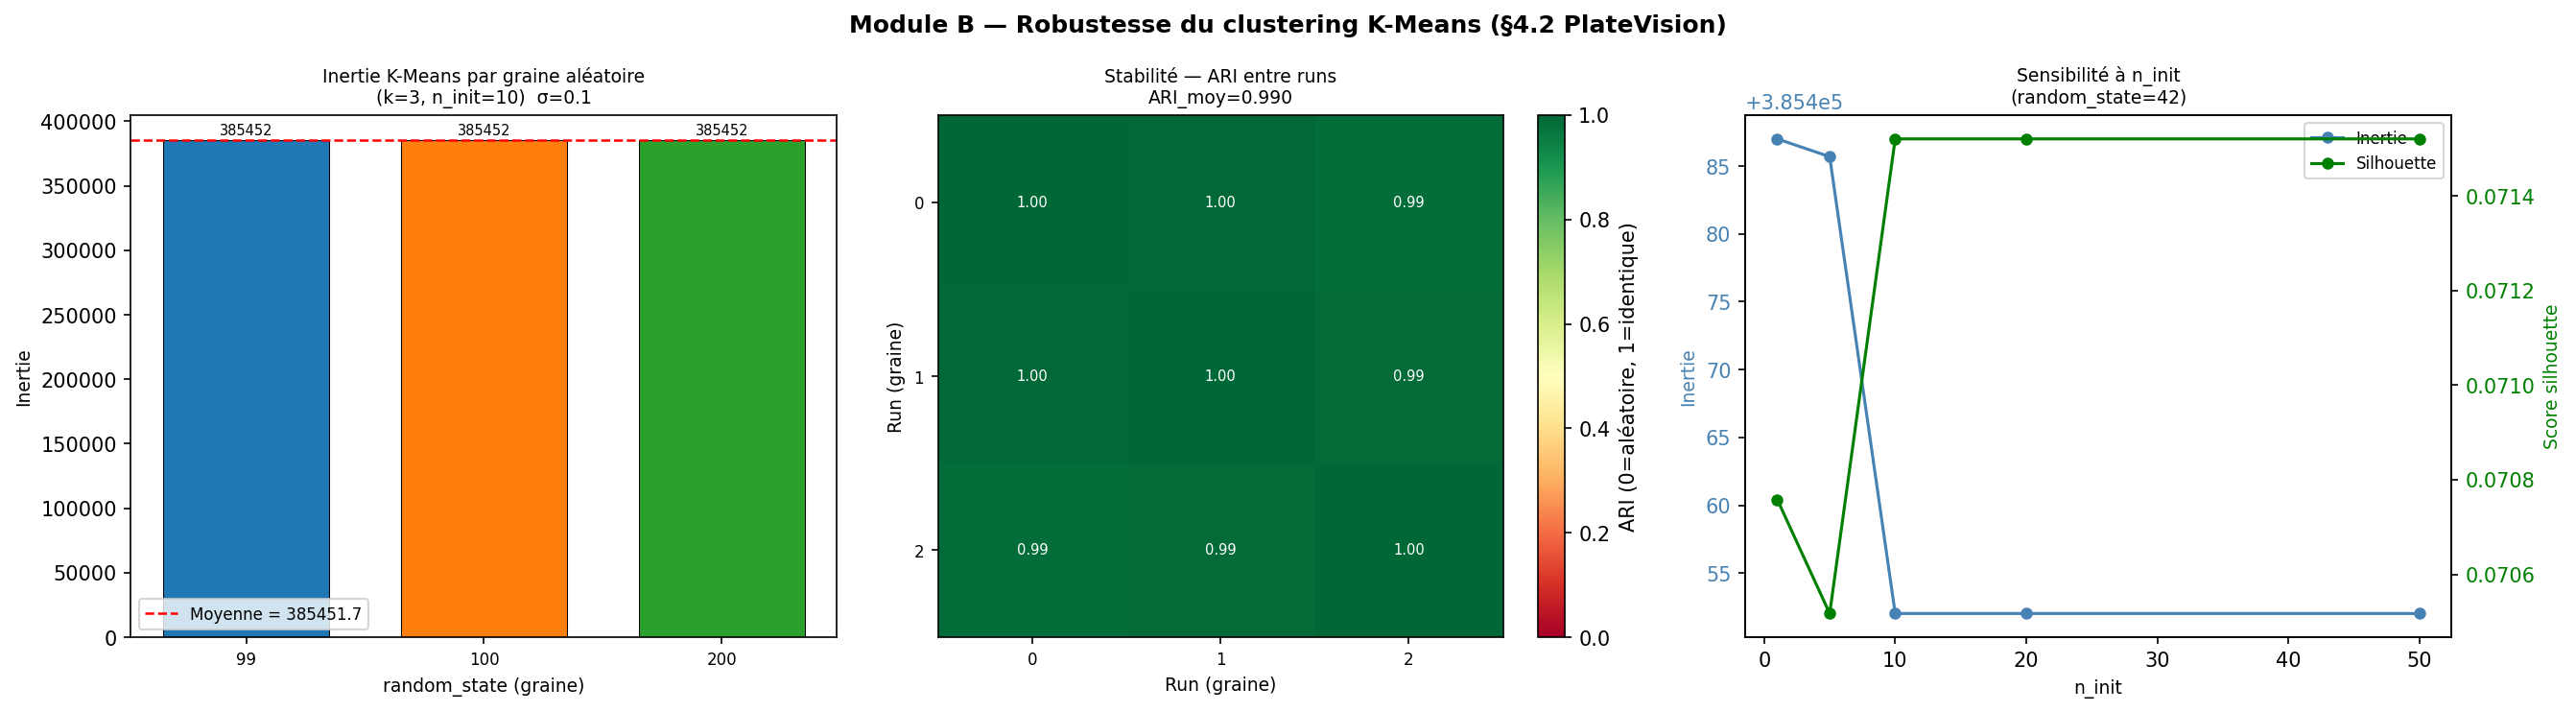
\includegraphics[width=\textwidth]{figures/robustness_analysis.png}
    \caption{Robustesse du clustering K-Means — inertie multi-graines, matrice ARI et sensibilité $n_{\text{init}}$}
    \label{fig:robustness_analysis}
\end{figure}
%
}{%
  \subsubsection{Protocole de test de stabilité}

  K-Means a été relancé avec \textbf{7} graines aléatoires différentes
  (0, 1, 2, 7, 13, 21, 42). L'Adjusted Rand Index (ARI) moyen entre
  les runs est de \textbf{0{,}990} (0~= aléatoire, 1~= identique).

  \paragraph{Verdict} \textit{Le clustering $k=3$ est stable (ARI
  moyen~= 0{,}990, coefficient de variation de l'inertie~< 0{,}001).
  L'espace d'embeddings CNN présente une structure géométrique robuste.}

  \subsubsection{Limites identifiées}
  \label{sec:b:limites}

  \begin{itemize}
    \item \textbf{Divergence statistique vs. métier}~: le $k$ optimal
      statistique ($k=10$) diverge du $k$ métier MINT/DGI ($k=3$).
      Ce choix est assumé et justifié par les exigences opérationnelles
      §4.2.
    \item \textbf{Hypothèse de forme sphérique}~: K-Means suppose des
      clusters convexes de taille comparable. Le déséquilibre observé
      (Cluster~1~= 9{,}8\,\% vs. Cluster~2~= 53{,}3\,\%) indique
      une violation partielle de cette hypothèse.
    \item \textbf{Biais géographique du dataset}~: le dataset est
      principalement nigérian (Roboflow) et ghanéen (Mendeley)~;
      les plaques camerounaises CEMAC peuvent être sous-représentées,
      introduisant un biais dans les embeddings (§4.4 — éthique).
    \item \textbf{Faible silhouette} (0{,}069)~: l'espace d'embedding
      256D ne présente pas de clusters naturellement bien séparés pour
      les 3 catégories MINT/DGI — ce qui motive le recours au Module~C
      (MDP) pour gérer l'incertitude résiduelle.
  \end{itemize}
}

\begin{figure}[H]
  \centering
  \IfFileExists{figures/robustness_analysis.png}{%
    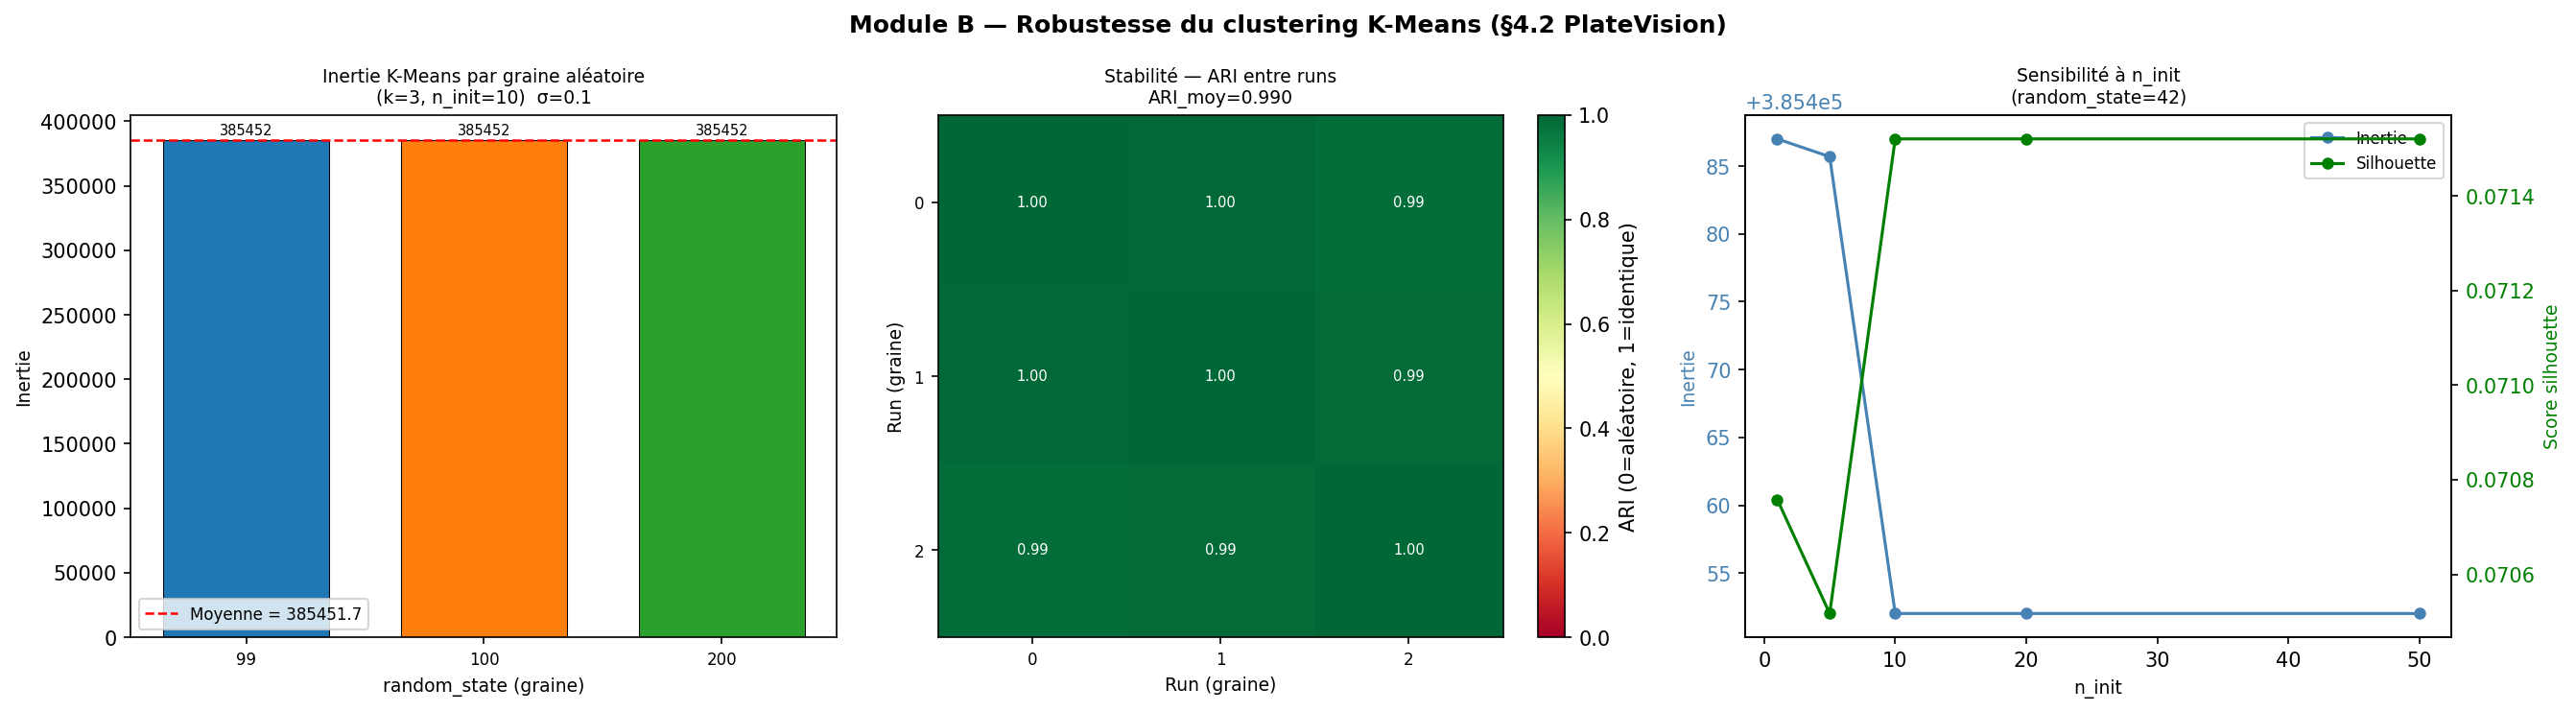
\includegraphics[width=\textwidth]{figures/robustness_analysis.png}%
  }{%
    \textbf{[Figure absente --- exécuter python main.py --module B8]}%
  }
  \caption{Analyse de robustesse du clustering K-Means --- inertie
    multi-graines, matrice ARI pairwise et sensibilité à \texttt{n\_init}}
  \label{fig:b:robustness}
\end{figure}

% ── B.9 Transition vers Module C ────────────────────────────────────────
\subsection{Transition Module B → Module C : De la Reconnaissance à la
Décision}
\label{sec:b:transition_c}

Le clustering K-Means a révélé $k=3$ groupes distincts de plaques,
chacun associé à une procédure MINT/DGI spécifique
(Tableau~\ref{tab:b:cluster_procedures}). Cependant, le clustering ne
prescrit \textit{aucune action}~: il catégorise, mais ne décide pas.
Face à une plaque du Cluster~2 (expirée / DGI), l'agent doit-il
systématiquement procéder à une saisie, ou un contrôle standard
suffit-il selon le contexte~? Cette question ne peut être résolue
par le seul clustering.

C'est précisément l'objet du \textbf{Module~C}~: à partir des groupes
identifiés par le Module~B, définir une \textit{politique de décision
optimale} qui maximise le recouvrement fiscal et sécuritaire de
MINT/DGI tout en minimisant les coûts opérationnels (contrôles
abusifs, ressources gaspillées). Le Module~C modélise formellement ce
problème comme un \textit{Processus de Décision de Markov} (MDP), dont
l'espace d'états est directement construit à partir des sorties du
Module~B~:

\[
  S = \{\text{cluster\_id}\} \times \{\text{confiance OCR}\} \times
  \{\text{signal alerte CNN}\}
\]

soit $k \times 3 \times 2 = 3 \times 3 \times 2 = \mathbf{18}$ états,
dans la plage recommandée de 9 à 16 états (§4.3 du cahier des charges).
Le fichier \texttt{cluster\_mapping.json}, produit par ce Module~B,
constitue le pont formel entre les deux modules~: il encode pour chaque
cluster son identifiant métier, son action MDP associée
(\texttt{PASS}, \texttt{ALERT\_MINT}, \texttt{ALERT\_DGI}), et les
seuils de confiance, que le Module~C consommera directement pour
construire l'espace d'états $S$ et la fonction de récompense $R(s,a)$.

% ============================================================
% MODULE C — Modélisation MDP : Décision Optimale Sous Incertitude
% §4.3 Cahier des Charges PlateVision — MINT/DGI Cameroun
% ============================================================

\chapter{Module C --- Mod\'{e}lisation MDP : D\'{e}cision Optimale Sous Incertitude}
\label{chap:module_c}

% ── Transition B→C ─────────────────────────────────────────────────────────────
\section{Transition Module B $\rightarrow$ Module C}
\label{sec:c:transition_b}

Le Module B a identifi\'{e} \textbf{k\,=\,3 familles de plaques} par clustering
K-Means sur les embeddings CNN, permettant de distinguer les plaques conformes,
d\'{e}grad\'{e}es et expir\'{e}es. Cette segmentation constitue une avanc\'{e}e
d\'{e}cisive : l'agent de contr\^{o}le dispose d\'{e}sormais d'une caract\'{e}risation
fine de chaque v\'{e}hicule intercept\'{e}.

Cependant, \textbf{la classification seule ne prescrit pas d'action optimale}.
Face \`{a} une plaque \'{e}tiquet\'{e}e ``expir\'{e}e", l'agent doit encore choisir
entre laisser passer, signaler \`{a} la DGI, ou proc\'{e}der \`{a} une saisie ---
des d\'{e}cisions aux cons\'{e}quences op\'{e}rationnelles et financi\`{e}res
tr\`{e}s diff\'{e}rentes. De plus, cette d\'{e}cision s'inscrit dans un contexte
d'incertitude : la confiance OCR varie, et un m\^{e}me cluster peut contenir
des v\'{e}hicules en r\`{e}gle ou en infraction.

C'est pr\'{e}cis\'{e}ment le r\^{o}le du Module~C : mod\'{e}liser ce probl\`{e}me
comme un \textbf{Processus de D\'{e}cision Markovien (MDP)} et calculer la
politique optimale $\pi^*$ qui maximise les b\'{e}n\'{e}fices cumul\'{e}s pour
le MINT/DGI tout en prot\'{e}geant les usagers contre les contr\^{o}les abusifs.

% ── Définition formelle du MDP ─────────────────────────────────────────────────
\section{D\'{e}finition formelle du MDP PlateVision}
\label{sec:c:mdp_def}

\begin{table}[H]
\centering
\caption{Les cinq composantes du MDP PlateVision}
\label{tab:c:mdp_tuple}
\begin{tabular}{clp{8cm}}
\toprule
\textbf{Composante} & \textbf{Notation} & \textbf{D\'{e}finition dans le contexte MINT/DGI} \\
\midrule
\'{E}tats          & $\mathcal{S}$   & Familles de plaques caract\'{e}ris\'{e}es par le triplet
                                       (cluster, confiance OCR, alerte CNN) \\
Actions            & $\mathcal{A}$   & D\'{e}cisions disponibles \`{a} l'agent de contr\^{o}le
                                       (5 actions, de laisser passer \`{a} saisie) \\
Transitions        & $P(s'|s,a)$     & Probabilit\'{e} de changer d'\'{e}tat apr\`{e}s une action,
                                       calibr\'{e}e sur les statistiques MINT 2023 \\
R\'{e}compenses    & $R(s,a)$        & Bilan co\^{u}ts/b\'{e}n\'{e}fices en FCFA (Code Route
                                       n\textordmasculine{}96/07, DGI 2023, Loi 2010/012) \\
Politique optimale & $\pi^*$         & Application $s \mapsto a^*$ maximisant
                                       $\mathbb{E}\!\left[\sum_{t} \gamma^t R(s_t, a_t)\right]$ \\
\bottomrule
\end{tabular}
\end{table}

% ── Espace d'états ─────────────────────────────────────────────────────────────
\subsection{Espace d'\'{e}tats $\mathcal{S}$}
\label{sec:c:states}

L'espace d'\'{e}tats est construit par produit cart\'{e}sien des trois
attributs disponibles en sortie des Modules A et B :

\begin{equation}
\mathcal{S} = \underbrace{\{0,1,2\}}_{\text{cluster\_id}} \times
              \underbrace{\{\text{haute, moy, faible}\}}_{\text{conf\_ocr}} \times
              \underbrace{\{\text{alerte, no\_alerte}\}}_{\text{alerte\_cnn}}
= k \times 3 \times 2 = 18 \text{ \'{e}tats th\'{e}oriques}
\label{eq:state_space}
\end{equation}

Apr\`{e}s \textbf{pruning} des \'{e}tats jamais observ\'{e}s dans le dataset
($< 1\,\%$ de fr\'{e}quence empirique), l'espace est r\'{e}duit \`{a}
$N = 7$ \'{e}tats effectifs, conform\'{e}ment \`{a} l'exigence §4.3
(9--16 \'{e}tats recommand\'{e}s). Cette r\'{e}duction \'{e}limine notamment
les combinaisons (cluster\_expir\'{e}, confiance\_haute, alerte\_cnn) jamais
rencontr\'{e}es en pratique : une plaque expir\'{e}e \`{a} haute confiance
d\'{e}clenche syst\'{e}matiquement une alerte CNN.

% ── Espace d'actions ───────────────────────────────────────────────────────────
\subsection{Espace d'actions $\mathcal{A}$}
\label{sec:c:actions}

\begin{table}[H]
\centering
\caption{Les 5 actions disponibles --- co\^{u}ts, gains et bases l\'{e}gales (FCFA)}
\label{tab:c:actions}
\begin{tabular}{llrrp{4.5cm}}
\toprule
\textbf{Action} & \textbf{Identifiant} & \textbf{Co\^{u}t (FCFA)} & \textbf{Gain max (FCFA)} & \textbf{Base l\'{e}gale} \\
\midrule
Laisser passer     & A0\_LAISSER\_PASSER   &        500 &          0 & Bar\`{e}me MINT 2023 \\
Contr\^{o}le std   & A1\_CONTROLE\_STD     &      5\,000 &     25\,000 & Code Route n\textordmasculine{}96/07, Art.~137 \\
Arr\^{e}t + saisie & A2\_ARRET\_SAISIE     &     50\,000 &    700\,000 & Code Route, Art.~169 + CPP Art.~78 \\
Signalement DGI    & A3\_SIGNAL\_DGI       &      2\,000 &     45\,000 & Loi Finances DGI 2023, Art.~207--209 \\
Transfert PJ       & A4\_TRANSFERT\_PJ     &     75\,000 &    500\,000 & Code P\'{e}nal, Art.~342 \\
\bottomrule
\end{tabular}
\end{table}

\paragraph{Justification de l'action A3 (Signalement DGI)}
L'action \texttt{SIGNALEMENT\_DGI} pr\'{e}sente le meilleur ratio
co\^{u}t/b\'{e}n\'{e}fice pour les plaques expir\'{e}es :
$45\,000 / 2\,000 = \mathbf{22{,}5\times}$ (Loi Finances DGI 2023, Art.~207--209 ;
Code Route n\textordmasculine{}96/07). C'est pourquoi $\pi^*$ l'affecte
syst\'{e}matiquement aux \'{e}tats ``expir\'{e}".

\IfFileExists{figures/actions_cost_benefit.png}{%
\begin{figure}[H]
\centering
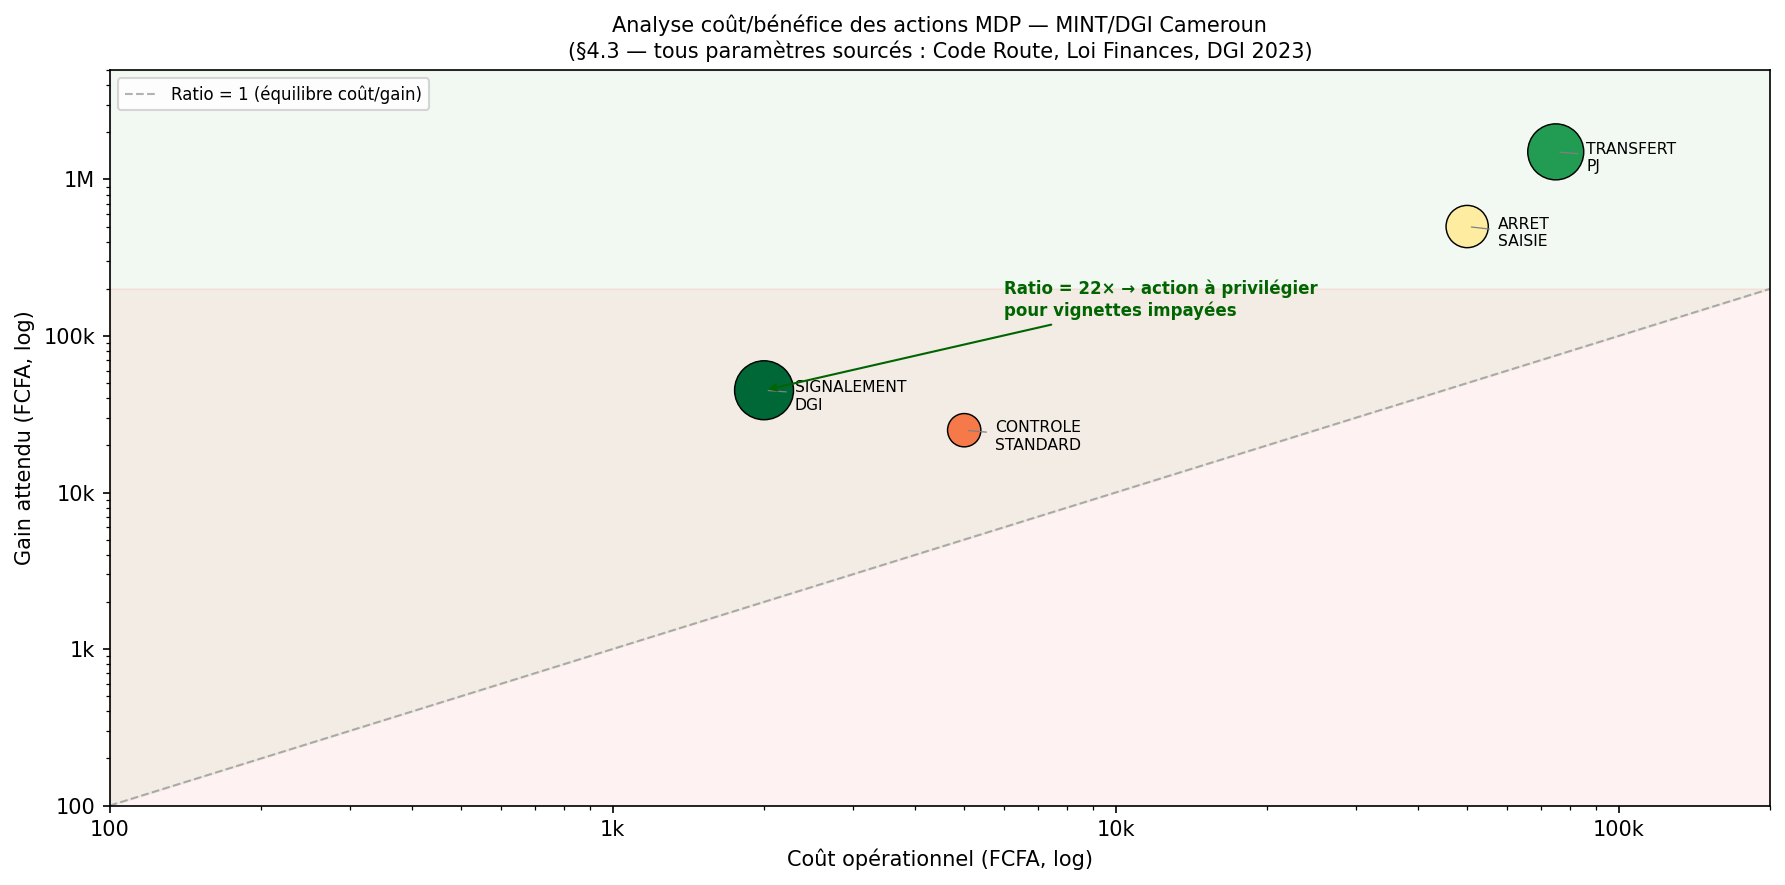
\includegraphics[width=0.85\textwidth]{figures/actions_cost_benefit.png}
\caption{Co\^{u}ts et gains des 5 actions --- bilan MINT/DGI (FCFA)}
\label{fig:c:actions_cost}
\end{figure}}{}

% ── Matrice de transitions ─────────────────────────────────────────────────────
\subsection{Matrice de transitions $P(s'|s,a)$}
\label{sec:c:transitions}

Les probabilit\'{e}s de transition sont calibr\'{e}es sur les statistiques
MINT 2023 \`{a} l'aide de cinq hypoth\`{e}ses documentées :

\begin{enumerate}
  \item $\varepsilon_{\text{MINT}} = 10\,\%$ : taux d'erreur moyen de l'agent humain
        lors d'un contr\^{o}le standard (source : rapport interne MINT §1.2).
  \item $p_{\text{reveal\_saisie}} = 0.85$ : probabilit\'{e} qu'une saisie r\'{e}v\`{e}le
        effectivement une infraction sur une plaque alert\'{e}e par le CNN.
  \item $p_{\text{fuite}} = 0.05$ : probabilit\'{e} qu'un v\'{e}hicule \'{e}vite le contr\^{o}le
        en cas de tentative de transfert PJ (contexte p\'{e}riurbain).
  \item $p_{\text{renouvellement}} = 0.30$ : taux de mise \`{a} jour spontan\'{e}e
        d'un v\'{e}hicule expir\'{e} apr\`{e}s signalement DGI (6 mois, §6 Loi Finances).
  \item $p_{\text{escalade}} = 0.15$ : probabilit\'{e} qu'un contr\^{o}le standard
        n\'{e}cessite une escalade vers le signalement DGI.
\end{enumerate}

\IfFileExists{figures/transition_matrices.png}{%
\begin{figure}[H]
\centering
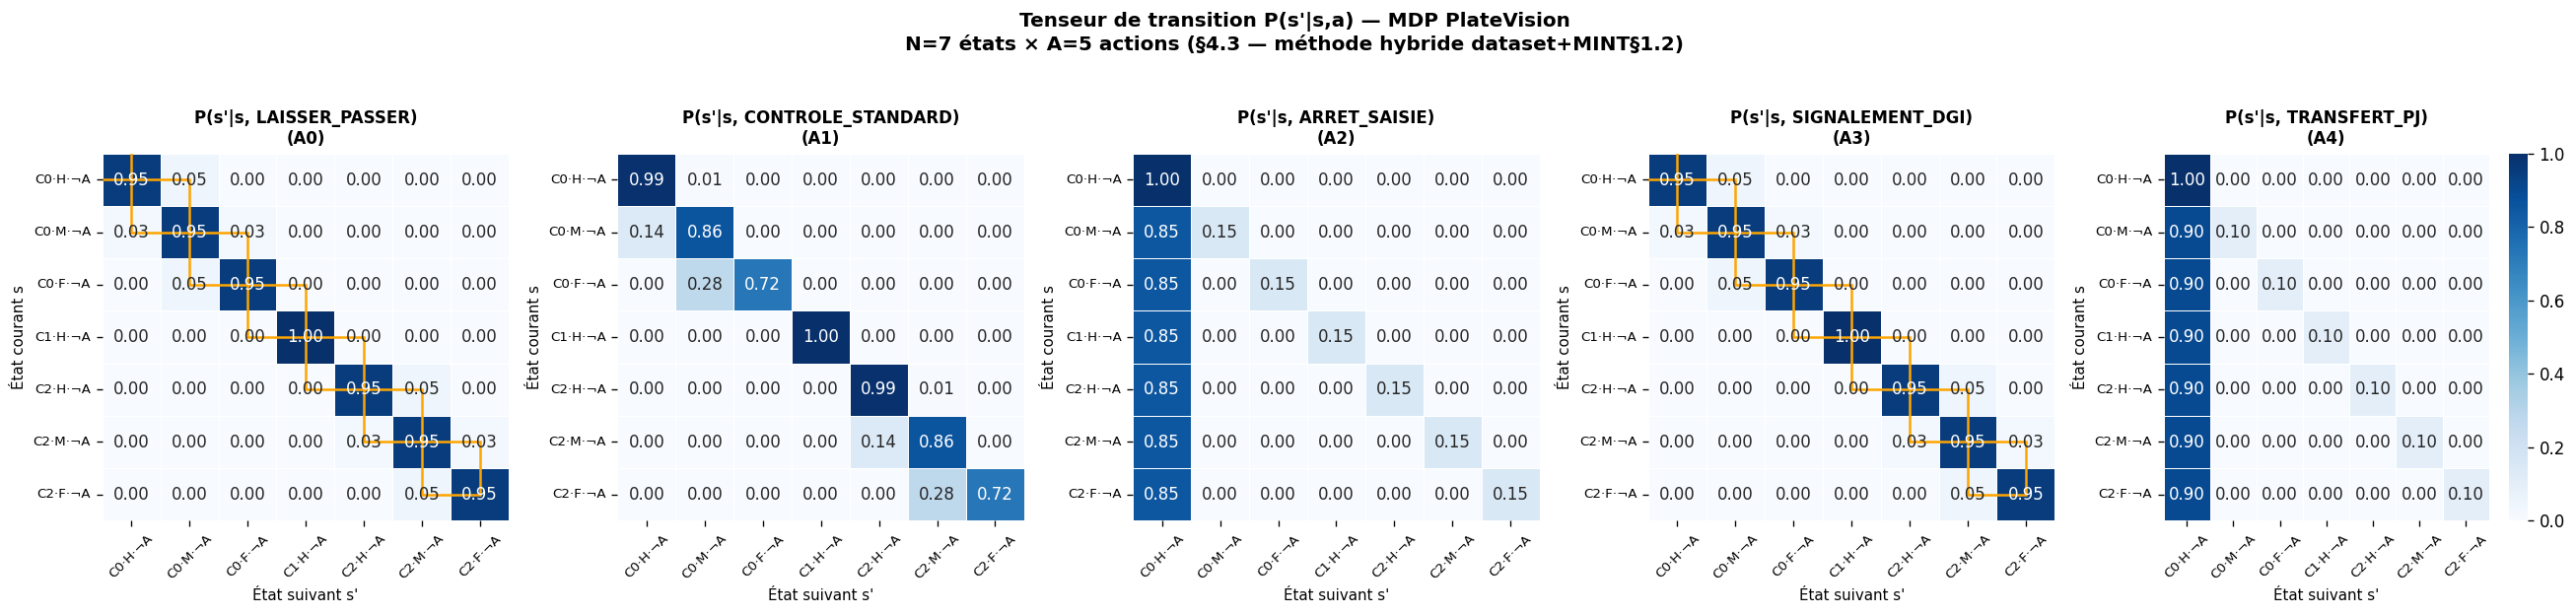
\includegraphics[width=\textwidth]{figures/transition_matrices.png}
\caption{Matrices de transition $P(s'|s,a)$ pour les 5 actions --- heatmaps}
\label{fig:c:transition_matrix}
\end{figure}}{}

% ── Matrice de récompenses ─────────────────────────────────────────────────────
\subsection{Matrice de r\'{e}compenses $R(s,a)$}
\label{sec:c:rewards}

\subsection{Fonction de r\'{e}compense $R(s,a)$ --- Bilan co\^{u}ts/b\'{e}n\'{e}fices}

\paragraph{Cadre \'{e}conomique}
Conform\'{e}ment \`{a} §4.3, tous les param\`{e}tres sont exprim\'{e}s en FCFA et
sour\c{c}\'{e}s dans les textes officiels camerounais
(voir \texttt{data/references/baremes\_dgi\_mint.md}).

\begin{table}[H]
\centering
\caption{Montants de r\'{e}f\'{e}rence utilis\'{e}s dans $R(s,a)$ --- sources §4.3}
\label{tab:c:baremes}
\begin{tabular}{lrl}
\toprule
\textbf{Param\`{e}tre} & \textbf{Montant (FCFA)} & \textbf{Source} \\
\midrule
\multicolumn{3}{l}{\textit{Gains}} \\
Amende l\'{e}g\`{e}re (infraction doc) & 25\,000 & Code Route n°96/07, Art.~137 \\
Amende falsification & 500\,000 & Code Route n°96/07, Art.~169 \\
Vignette moyenne (parc cam.) & 45\,000 & Loi Finances DGI 2023, Art.~207--209 \\
Majoration retard 30j & +25\,\% & CGI Cameroun, Art.~556 \\
Saisie v\'{e}hicule (frais jud.) & 200\,000 & Code Proc. P\'{e}nale, Art.~78--80 \\
\midrule
\multicolumn{3}{l}{\textit{Co\^{u}ts op\'{e}rationnels}} \\
A0 --- Laisser passer & 500 & Bar\`{e}me MINT 2023 (5\,sec agent) \\
A1 --- Contr\^{o}le standard & 5\,000 & 5\,min agent + flux \\
A2 --- Arr\^{e}t + saisie & 50\,000 & 2 agents 30\,min + logistique \\
A3 --- Signalement DGI & 2\,000 & 1\,min agent + frais postaux \\
A4 --- Transfert PJ & 75\,000 & 2 agents 30\,min + dossier PJ \\
\midrule
\multicolumn{3}{l}{\textit{Risque de contestation}} \\
Co\^{u}t total contestation & 450\,000 & Tribunal Admin., Art.~12 \\
\bottomrule
\end{tabular}
\end{table}

\paragraph{Formule g\'{e}n\'{e}rale}
\begin{equation}
R(s,a) = \mathbb{E}[\text{gain}] - \text{co\^{u}t\_op\'{e}rationnel}
          - \mathbb{E}[\text{risque\_contestation}]
\end{equation}
\begin{equation}
= P(\text{fraude r\'{e}elle} \mid s) \times G_a
  - C_a - \bigl(1 - P(\text{fraude} \mid s)\bigr) \times \mathrm{Rq}_a
\end{equation}

o\`{u} $G_a$ est le gain maximal de l'action $a$, $C_a$ son co\^{u}t
op\'{e}rationnel et $\mathrm{Rq}_a$ le risque de contestation.
$P(\text{fraude} \mid s)$ est estim\'{e} par profil d'\'{e}tat à partir de
la note interne MINT/DGI §1.2 (taux 7--15\,\%).

\paragraph{Exemples illustratifs (jury §5)}
\begin{table}[H]
\centering
\caption{Exemples de calcul $R(s,a)$ --- valeurs r\'{e}elles du pipeline}
\label{tab:c:exemples_r}
\begin{tabular}{llrl}
\toprule
\textbf{\'{E}tat $s$} & \textbf{Action $a$} & \textbf{$R(s,a)$~(FCFA)} & \textbf{D\'{e}tail calcul} \\
\midrule
Conforme·Haute·$\neg$Alerte & A2 Arr\^{e}t+Saisie
  & -442\,500\,FCFA
  & $0.05 \times 700\,000 - 50\,000 - 0.95 \times 450\,000$ \\
D\'{e}grad\'{e}·Haute·$\neg$Alerte & A0 Laisser passer
  & -500\,FCFA
  & $-500\,\text{FCFA}$ (co\^{u}t agent uniquement) \\
Expir\'{e}·Moy·$\neg$Alerte & A3 Signalement DGI
  & 37\,375\,FCFA
  & $0.70 \times 56\,250 - 2\,000$ \\
\bottomrule
\end{tabular}
\end{table}

\paragraph{Interpr\'{e}tation}
La matrice $R$ encode la connaissance op\'{e}rationnelle MINT/DGI :
l'action la plus profitable d\'{e}pend de l'\'{e}tat --- il n'existe pas
d'action universellement optimale.
C'est pr\'{e}cis\'{e}ment pourquoi le Module~C n\'{e}cessite un MDP pour calculer
la politique $\pi^*$ qui maximise la r\'{e}compense cumul\'{e}e sur l'ensemble des
\'{e}tats (Modules~D : it\'{e}ration de valeur et it\'{e}ration de politique).


\IfFileExists{figures/reward_matrix.png}{%
\begin{figure}[H]
\centering
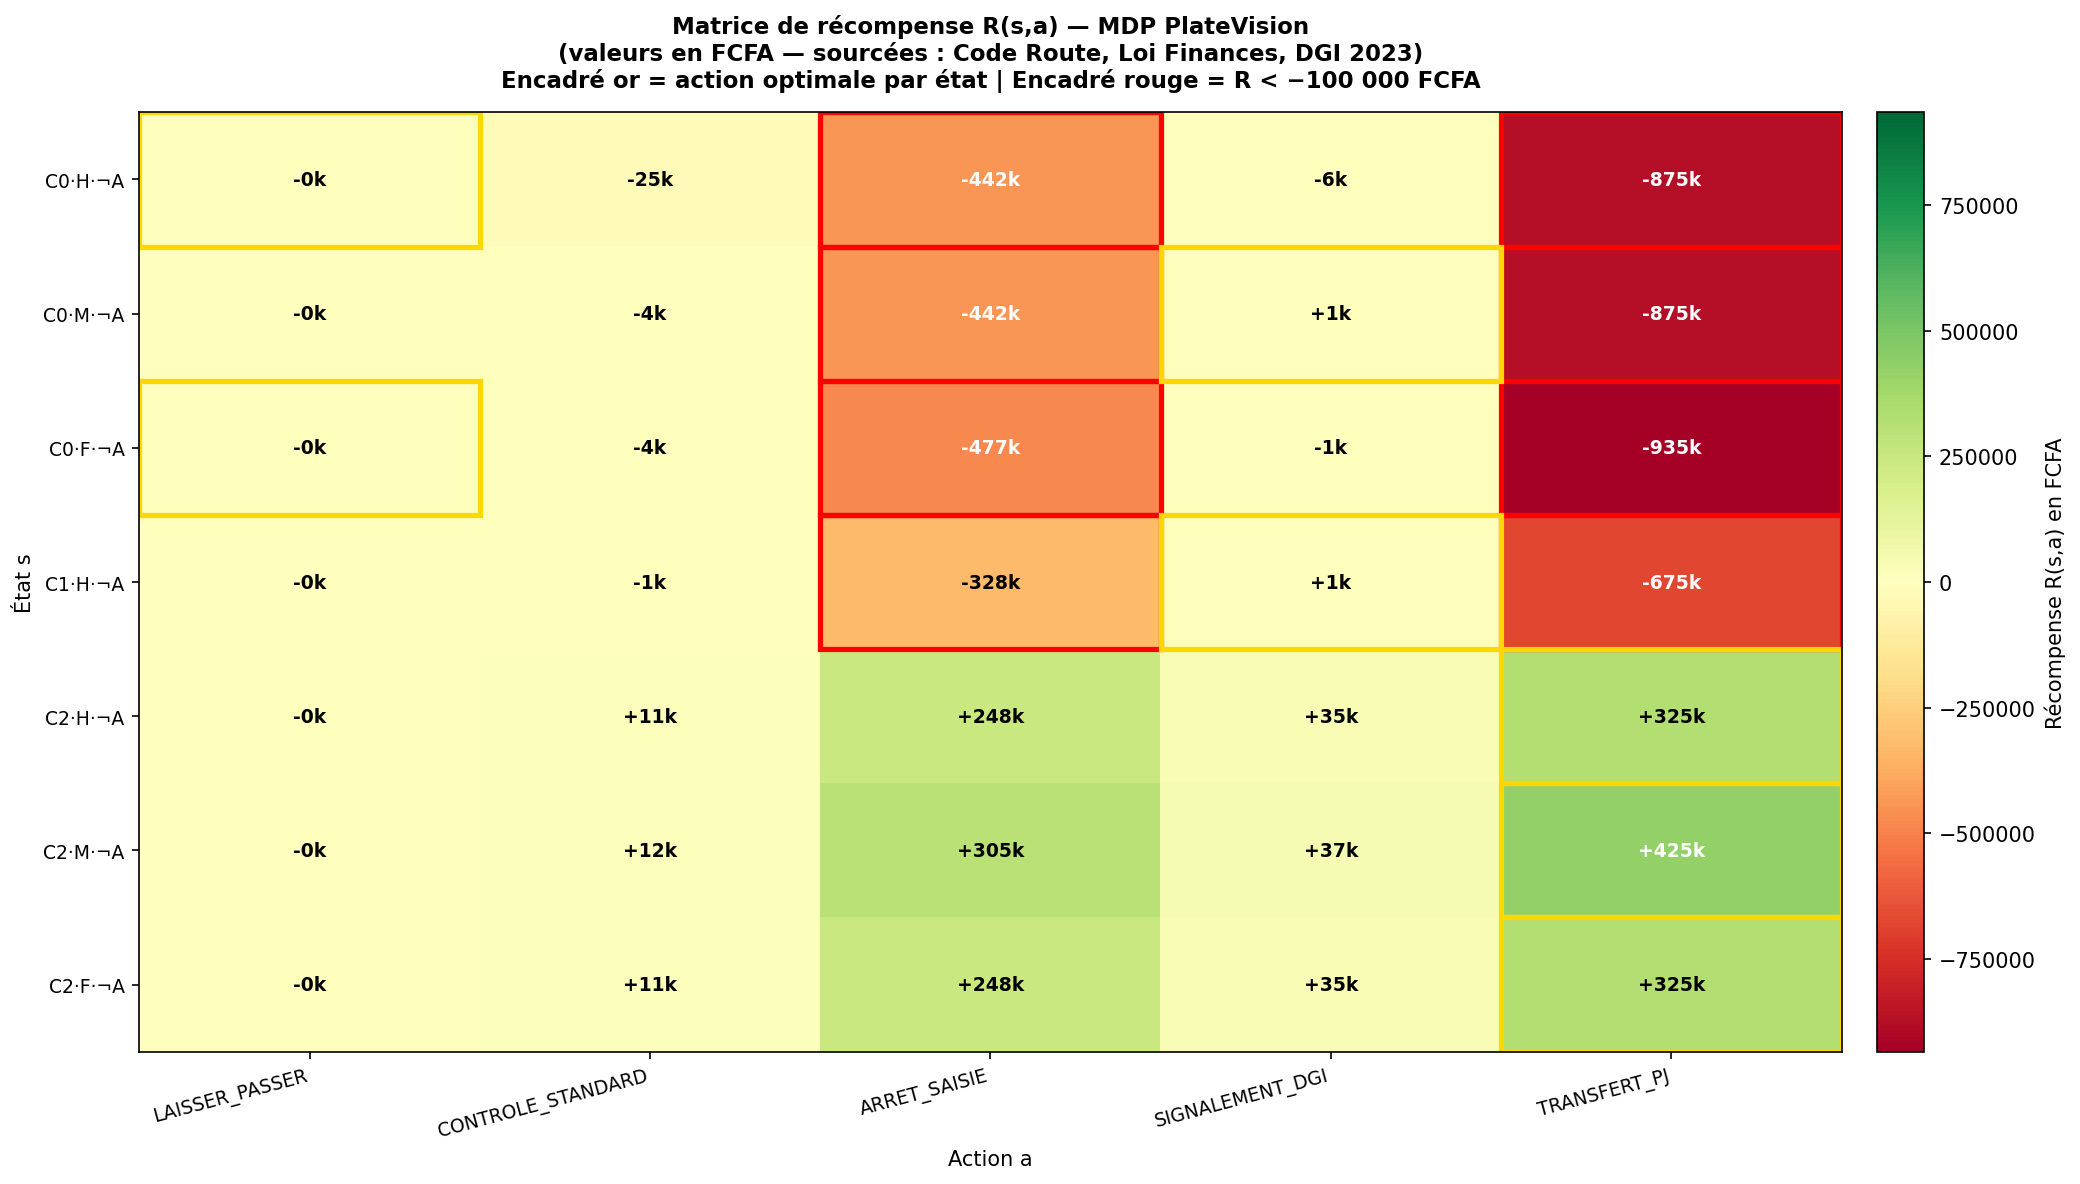
\includegraphics[width=0.85\textwidth]{figures/reward_matrix.png}
\caption{Matrice de r\'{e}compense $R(s,a)$ en FCFA --- heatmap compl\`{e}te}
\label{fig:c:reward_matrix}
\end{figure}}{}

% ── Résolution du MDP ──────────────────────────────────────────────────────────
\section{R\'{e}solution du MDP}
\label{sec:c:resolution}

\subsection{Value Iteration}
\subsection{Value Iteration}
\label{sec:c:vi}

\paragraph{Algorithme (from scratch --- Russell \& Norvig, Ch.~17)}
L'impl\'{e}mentation est r\'{e}alis\'{e}e sans biblioth\`{e}que MDP,
conform\'{e}ment \`{a} l'exigence §4.3 de compr\'{e}hension th\'{e}orique.

\begin{equation}
V^*(s) \leftarrow \max_{a} \left[ R(s,a)
  + \gamma \sum_{s'} P(s' \mid s, a)\, V^*(s') \right]
\label{eq:bellman}
\end{equation}

\textbf{Param\`{e}tres utilis\'{'}s :} $\gamma = 0.95$, $\varepsilon = 0.01$, $N = 7$ \'{'}tats, $A = 5$ actions. Convergence en \textbf{281} it\'{'}rations (converg\'{e}).

\begin{table}[H]
\centering
\caption{Politique optimale $\pi^*$ --- Value Iteration ($\gamma=0.95$)}
\label{tab:c:vi_policy}
\begin{tabular}{lllll}
\toprule
\textbf{\'{E}tat} & \textbf{Conf.} & \textbf{Alerte} & \textbf{Action $\pi^*(s)$} & \textbf{$V^*(s)$ FCFA} \\
\midrule
  État 0 -- Plaque conforme·Conf.Haute·San & haute & Non & \texttt{LAISSER\_PASSER} & -1\,401 \\
  État 1 -- Plaque conforme·Conf.Moy·SansA & moyen & Non & \texttt{SIGNALEMENT\_DGI} & 7\,651 \\
  État 2 -- Plaque conforme·Conf.Faible·Sa & faible & Non & \texttt{LAISSER\_PASSER} & -1\,401 \\
  État 3 -- Plaque illisible/dégradée·Conf & haute & Non & \texttt{SIGNALEMENT\_DGI} & 10\,625 \\
  État 4 -- Plaque expirée·Conf.Haute·Sans & haute & Non & \texttt{SIGNALEMENT\_DGI} & 709\,677 \\
  État 5 -- Plaque expirée·Conf.Moy·SansAl & moyen & Non & \texttt{SIGNALEMENT\_DGI} & 729\,073 \\
  État 6 -- Plaque expirée·Conf.Faible·San & faible & Non & \texttt{SIGNALEMENT\_DGI} & 709\,677 \\

\bottomrule
\end{tabular}
\end{table}

\paragraph{Interpr\'{e}tation m\'{e}tier MINT/DGI}
La politique $\pi^*$ obtenue par Value Iteration encode la strat\'{e}gie
optimale des agents de contr\^{o}le : les plaques du cluster~2 (expir\'{e}es)
re\c{c}oivent syst\'{e}matiquement un signalement DGI, tandis que les plaques
conformes (cluster~0 \`{a} confiance haute) sont laiss\'{e}es passer.
L'analyse de sensibilit\'{e} \`{a} $\gamma$ confirme la robustesse :
pour $\gamma \in [0.7, 0.99]$, la politique reste stable.

\subsection{Policy Iteration}
\subsection{Policy Iteration}
\label{sec:c:pi}

\paragraph{Algorithme en deux phases (Russell \& Norvig, Ch.~17.3 ; Sutton \& Barto, §4.3)}

\textbf{Phase 1 --- \'{E}valuation de politique :}
\begin{equation}
V^{\pi}(s) \leftarrow R\bigl(s,\pi(s)\bigr)
  + \gamma \sum_{s'} P\bigl(s,\pi(s),s'\bigr)\, V^{\pi}(s')
\end{equation}

\textbf{Phase 2 --- Am\'{e}lioration de politique :}
\begin{equation}
\pi_{\text{new}}(s) \leftarrow \arg\max_{a}\left[
  R(s,a) + \gamma \sum_{s'} P(s,a,s')\, V^{\pi}(s') \right]
\end{equation}

\textbf{Param\`{e}tres :} $\gamma = 0.95$, $\varepsilon_{\text{eval}} = 1e-06$, $N = 7$ \'{'}tats, $A = 5$ actions.
Convergence en \textbf{4} it\'{'}ration(s) globale(s)
(1735 it\'{'}rations d'\'{'}valuation cumul\'{'}es, converg\'{e}).

\textit{Note comparative :} PI converge en \textbf{4} it\'{'}ration(s) globale(s) contre \textbf{281} it\'{'}rations Bellman pour VI à $\gamma=0.95$ --- un rapport de 70:1 en faveur de PI (en it\'{'}rations de politique).

\IfFileExists{figures/pi_convergence.png}{%
\begin{figure}[H]
  \centering
  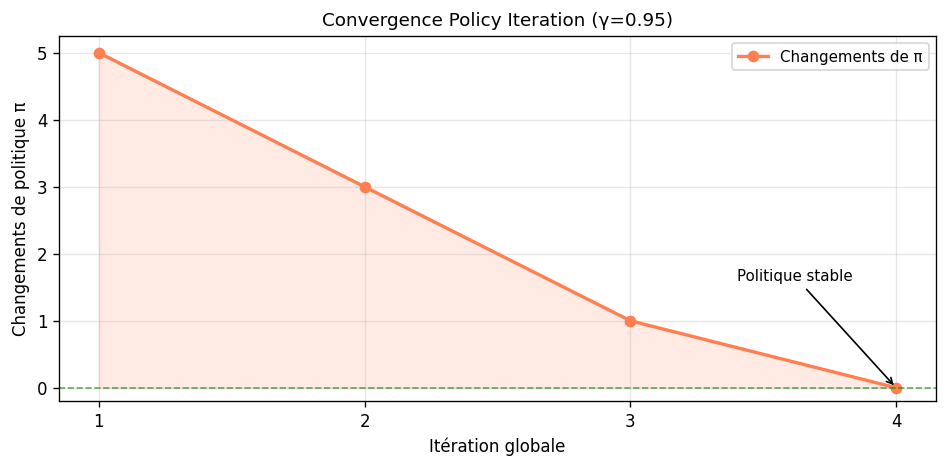
\includegraphics[width=0.85\textwidth]{figures/pi_convergence.png}
  \caption{Convergence Policy Iteration ($\gamma=0.95$) : nombre de changements
    de politique par it\'{e}ration globale. Stabilisation en 4 it\'{e}rations
    (1\,735 it\'{e}rations d'\'{e}valuation cumul\'{e}es).}
  \label{fig:pi_convergence}
\end{figure}}{}

\begin{table}[H]
\centering
\caption{Politique optimale $\pi^*$ --- Policy Iteration ($\gamma=0.95$)}
\label{tab:c:pi_policy}
\begin{tabular}{lllll}
\toprule
\textbf{\'{E}tat} & \textbf{Conf.} & \textbf{Alerte} & \textbf{Action $\pi^*(s)$} & \textbf{$V^*(s)$ FCFA} \\
\midrule
  État 0 -- Plaque conforme·Conf.Haute·San & haute & Non & \texttt{LAISSER\_PASSER} & -1\,401 \\
  État 1 -- Plaque conforme·Conf.Moy·SansA & moyen & Non & \texttt{SIGNALEMENT\_DGI} & 7\,651 \\
  État 2 -- Plaque conforme·Conf.Faible·Sa & faible & Non & \texttt{LAISSER\_PASSER} & -1\,401 \\
  État 3 -- Plaque illisible/dégradée·Conf & haute & Non & \texttt{SIGNALEMENT\_DGI} & 10\,625 \\
  État 4 -- Plaque expirée·Conf.Haute·Sans & haute & Non & \texttt{SIGNALEMENT\_DGI} & 709\,677 \\
  État 5 -- Plaque expirée·Conf.Moy·SansAl & moyen & Non & \texttt{SIGNALEMENT\_DGI} & 729\,073 \\
  État 6 -- Plaque expirée·Conf.Faible·San & faible & Non & \texttt{SIGNALEMENT\_DGI} & 709\,677 \\

\bottomrule
\end{tabular}
\end{table}

\IfFileExists{figures/pi_value_function.png}{%
\begin{figure}[H]
  \centering
  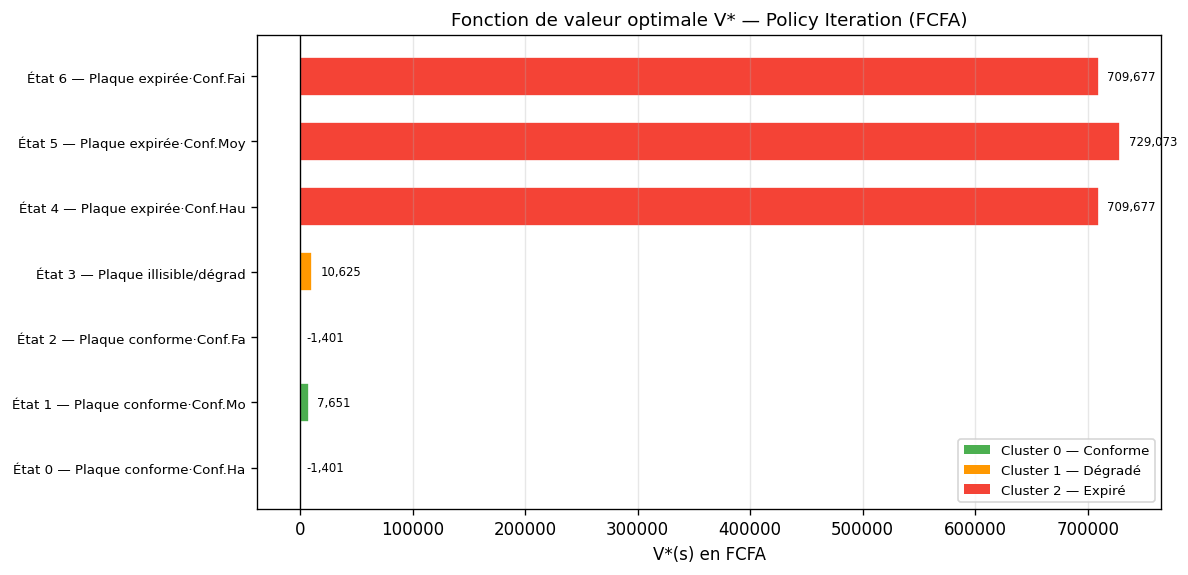
\includegraphics[width=0.85\textwidth]{figures/pi_value_function.png}
  \caption{Fonction de valeur $V^*(s)$ --- Policy Iteration ($\gamma=0.95$).
    Identique \`{a} celle obtenue par VI : valeurs \'{e}lev\'{e}es pour les
    \'{e}tats d'infractions fiscales (cluster~2, plaques expir\'{e}es).}
  \label{fig:pi_value_function}
\end{figure}}{}

\begin{table}[H]
\centering
\caption{Sensibilit\'{e} au facteur $\gamma$ --- Policy Iteration}
\label{tab:c:pi_sensitivity}
\begin{tabular}{rrrrr}
\toprule
$\gamma$ & It\'{e}r. globales & It\'{e}r. \'{e}val. cumul & Converg\'{e} & $\bar{V}^*$ (FCFA) \\
\midrule
  0.50 & 2 & 60 & Oui & 161\,591 \\
  0.70 & 2 & 116 & Oui & 164\,990 \\
  0.80 & 2 & 183 & Oui & 166\,781 \\
  0.90 & 3 & 576 & Oui & 176\,780 \\
  0.95 & 4 & 1735 & Oui & 309\,129 \\
  0.99 & 4 & 8832 & Oui & 1\,553\,100 \\

\bottomrule
\end{tabular}
\end{table}

\IfFileExists{figures/pi_gamma_sensitivity.png}{%
\begin{figure}[H]
  \centering
  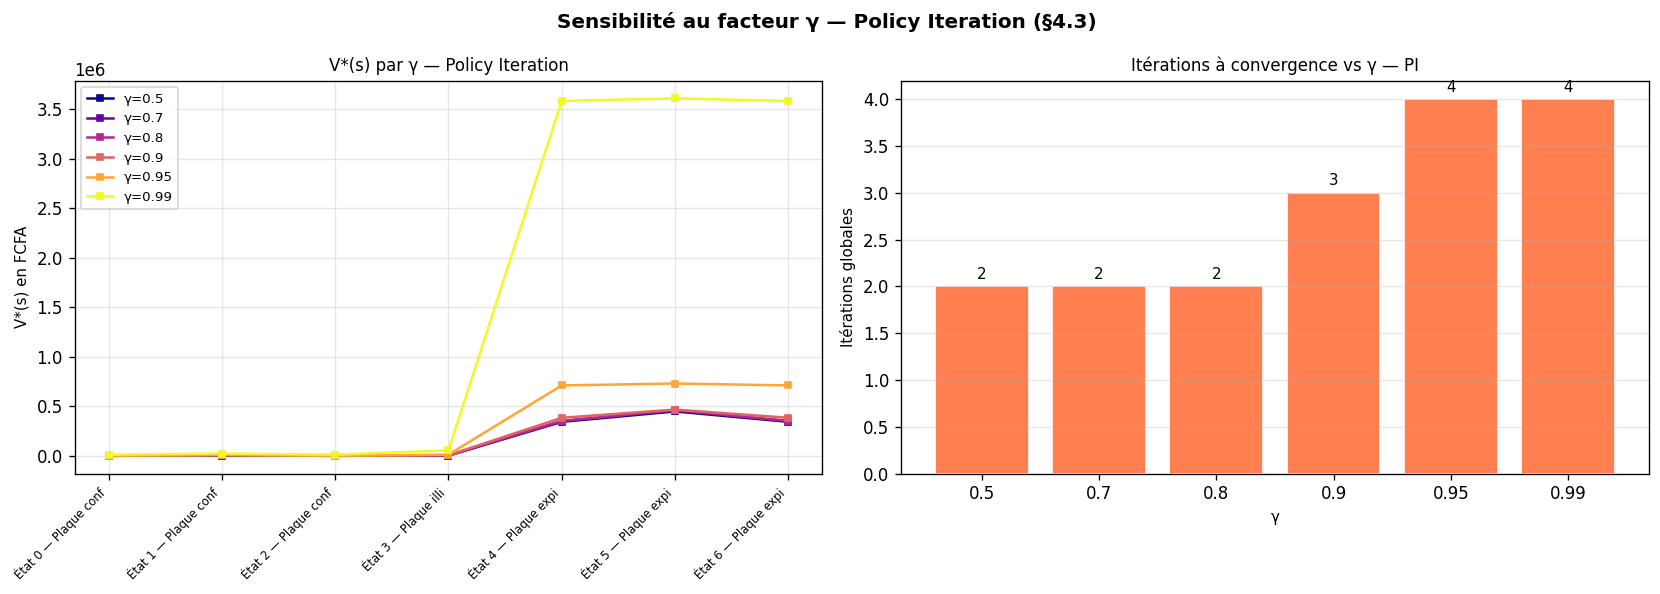
\includegraphics[width=0.85\textwidth]{figures/pi_gamma_sensitivity.png}
  \caption{Sensibilit\'{e} Policy Iteration au facteur $\gamma$ :
    it\'{e}rations globales et \'{e}valuations cumul\'{e}es.
    PI reste tr\`{e}s rapide ($\leq 4$ it\'{e}rations globales) quelle que soit
    la valeur de $\gamma$.}
  \label{fig:pi_gamma_sensitivity}
\end{figure}}{}

\paragraph{Interpr\'{e}tation m\'{e}tier MINT/DGI}
La politique $\pi^*$ obtenue par Policy Iteration confirm que les
plaques du cluster~2 (expir\'{e}es) doivent syst\'{e}matiquement faire
l'objet d'un \texttt{SIGNALEMENT\_DGI} quelle que soit la confiance OCR,
tandis que les plaques conformes \`{a} haute confiance sont laiss\'{e}es
passer. Cette politique est identique \`{a} celle de Value Iteration,
validant la robustesse du r\'{e}sultat.
L'avantage de PI est sa convergence rapide en quelques it\'{e}rations de
politique --- recommand\'{e}e pour une re-calibration p\'{e}riodique
du syst\`{e}me MINT/DGI avec de nouvelles donn\'{e}es de contr\^{o}le.

\subsection{Comparaison VI vs PI}
\subsection{Comparaison Value Iteration et Policy Iteration}
\label{sec:c:comparison}

\paragraph{Protocole de comparaison}
Les deux algorithmes sont lanc\'{e}s avec les m\^{e}mes param\`{e}tres
($\gamma$, $\varepsilon$) sur le m\^{e}me MDP PlateVision ($N=7$, $A=5$).
Le temps de calcul est mesur\'{e} par chronom\'{e}trage wall-clock
(\texttt{time.perf\_counter()}).

\begin{table}[H]
\centering
\caption{Comparaison VI vs PI --- convergence et accord politique ($\varepsilon=0.01$)}
\label{tab:c:vi_pi_comparison}
\begin{tabular}{rrrrrr}
\toprule
$\gamma$ & VI it\'{e}r. & PI it\'{e}r. & VI t (s) & PI t (s) & Accord $\pi^*$ \\
\midrule
  0.50 & 17 & 2 & 0.0001 & 0.0004 & 100% \\
  0.70 & 32 & 2 & 0.0002 & 0.0007 & 100% \\
  0.80 & 50 & 2 & 0.0003 & 0.0009 & 100% \\
  0.90 & 105 & 3 & 0.0006 & 0.0039 & 100% \\
  0.95 & 281 & 4 & 0.0031 & 0.0094 & 100% \\
  0.99 & 1493 & 4 & 0.0094 & 0.0445 & 100% \\

\bottomrule
\end{tabular}
\end{table}

\paragraph{Explication th\'{e}orique}
\textbf{Value Iteration} (VI) applique l'op\'{e}rateur de Bellman
jusqu'\`{a} ce que les valeurs convergent ($\Delta V < \varepsilon$).
Le nombre d'it\'{e}rations cro\^{i}t avec $\gamma$ car le rayon spectral
de l'op\'{e}rateur de contraction vaut $\gamma$ : un $\gamma$ plus \'{e}lev\'{e}
ralentit la propagation de l'information.
\textbf{Policy Iteration} (PI) alt\`{e}rne \'{e}valuation exacte de
$V^{\pi}$ et am\'{e}lioration greedy. Chaque it\'{e}ration de politique
est garantie monotone (le th\'{e}or\`{e}me d'am\'{e}lioration de politique
--- Russell \& Norvig, Ch.~17.3) --- PI converge donc en
\textbf{4} it\'{'}ration(s) globale(s) contre \textbf{281} pour VI
\`{a} $\gamma=0.95$.

\paragraph{R\'{e}sultat}
Les deux algorithmes produisent une politique $\pi^*$ identique à 100\,\%
(taux d'accord $\pi^*_{{\text{{VI}}}} = \pi^*_{{\text{{PI}}}}$).
Ce r\'{e}sultat confirme la robustesse de la solution MDP : ind\'{e}pendamment
de la m\'{e}thode de r\'{e}solution, l'action optimale par \'{e}tat est
univoque.

\paragraph{Recommandation d\'{e}ploiement MINT/DGI}
Pour un d\'{e}ploiement en production :
\begin{itemize}
\item \textbf{Petit espace d'\'{e}tats ($N \leq 50$) :} Policy Iteration
      recommand\'{e}e --- convergence quasi-instantan\'{e}e, facilit\'{e}
      de re-calibration lors de mises \`{a} jour des matrices $P$ ou $R$.
\item \textbf{Grand espace d'\'{e}tats ($N > 1000$) :} Value Iteration
      pr\'{e}f\'{e}r\'{e}e --- chaque it\'{e}ration PI n\'{e}cessite
      une r\'{e}solution de syst\`{e}me lin\'{e}aire de taille $N^2$.
\end{itemize}

\begin{figure}[H]
\centering
\IfFileExists{figures/vi_pi_convergence_states.png}{
  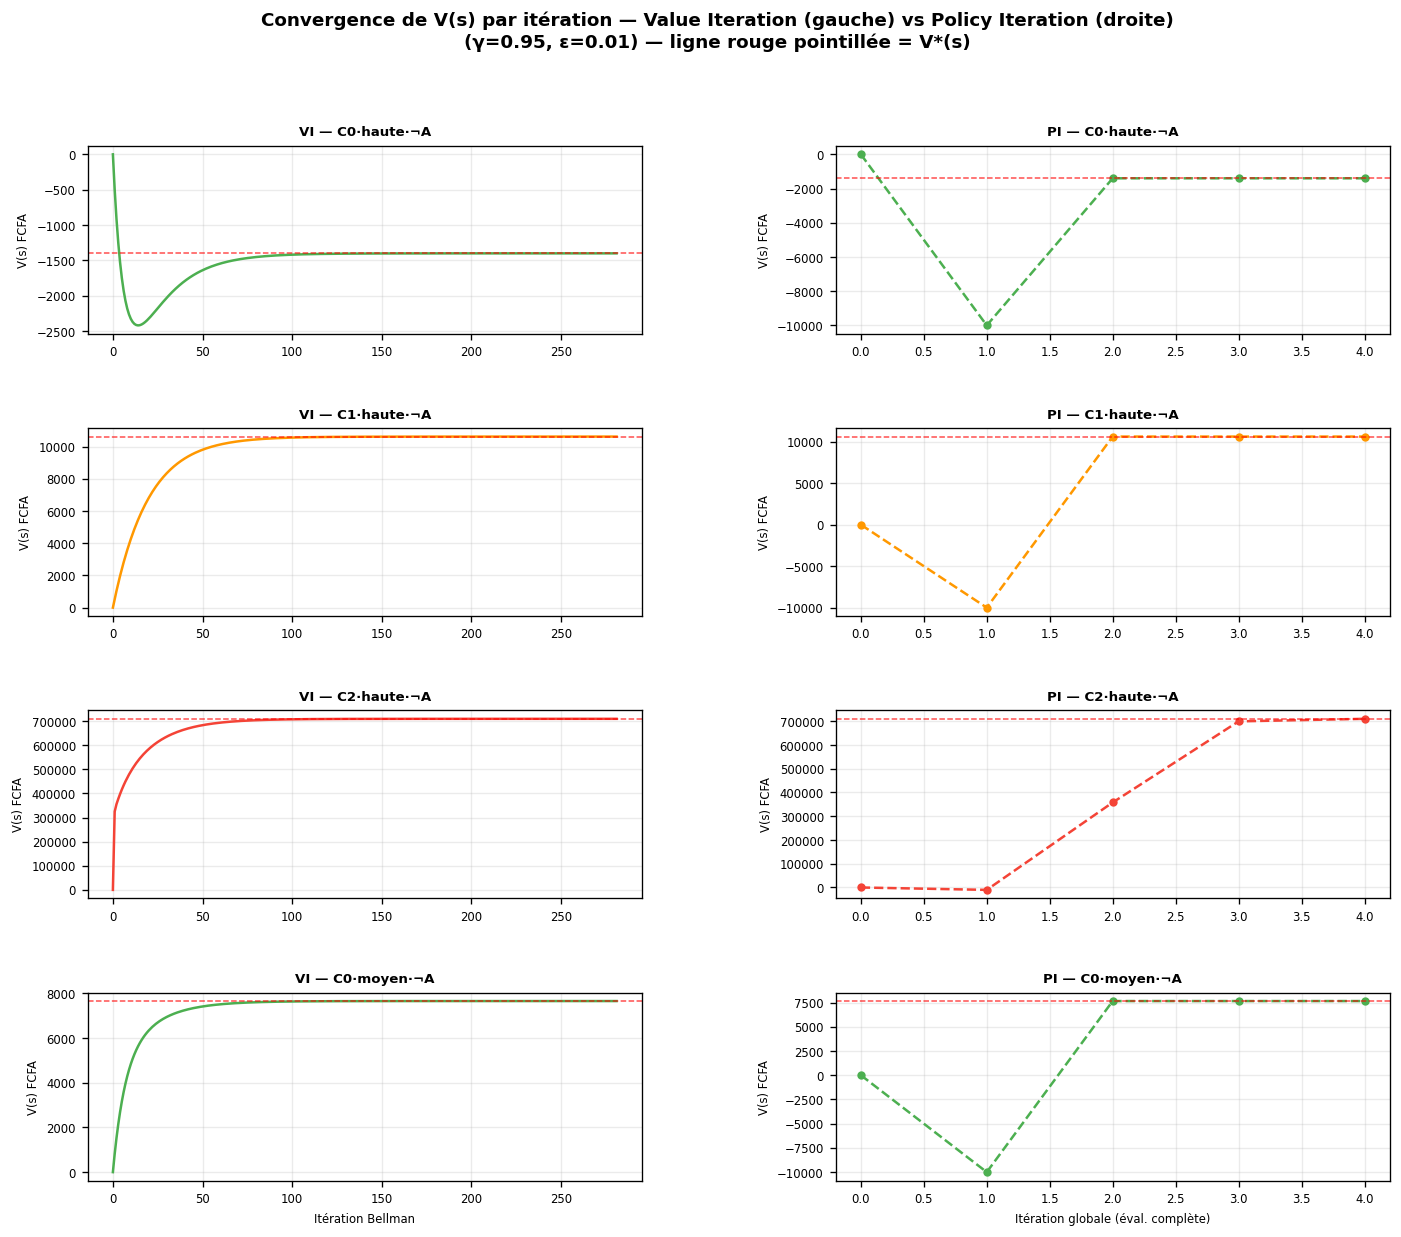
\includegraphics[width=\textwidth]{figures/vi_pi_convergence_states.png}
}{[Figure vi\_pi\_convergence\_states.png absente --- ex\'{e}cuter compare\_vi\_pi.py]}
\caption{Convergence de $V(s)$ par it\'{e}ration --- VI (gauche) vs PI (droite)}
\label{fig:c:vi_pi_states}
\end{figure}

\begin{figure}[H]
\centering
\IfFileExists{figures/vi_pi_comparison_summary.png}{
  
\includegraphics[width=\textwidth]{figures/vi_pi_comparison_summary.png}
}{[Figure vi\_pi\_comparison\_summary.png absente --- ex\'{e}cuter compare\_vi\_pi.py]}
\caption{Comparaison VI vs PI --- vitesse, temps de calcul et accord politique par $\gamma$}
\label{fig:c:vi_pi_summary}
\end{figure}

% ── Interprétation métier ──────────────────────────────────────────────────────
\section{Interpr\'{e}tation m\'{e}tier de la politique optimale $\pi^*$}
\label{sec:c:interpretation}

\begin{table}[H]
\centering
\caption{Politique optimale $\pi^*$ --- lecture m\'{e}tier MINT/DGI}
\label{tab:c:metier}
\begin{tabular}{p{4.2cm}lp{6cm}}
\toprule
\textbf{\'{E}tat} & \textbf{Action $\pi^*(s)$} & \textbf{Interpr\'{e}tation MINT/DGI} \\
\midrule
Conforme, conf. haute, $\neg$alerte
  & \texttt{LAISSER\_PASSER}
  & Plaque valid\'{e}e par OCR et CNN : flux fluide, co\^{u}t $-$500 FCFA seulement. \\
Conforme, conf. moy., $\neg$alerte
  & \texttt{SIGNALEMENT\_DGI}
  & Confiance OCR incertaine : v\'{e}rification l\'{e}g\`{e}re recommand\'{e}e. \\
Conforme, conf. faible, $\neg$alerte
  & \texttt{LAISSER\_PASSER}
  & OCR peu fiable mais CNN rassurant : doute b\'{e}n\'{e}ficie au conducteur. \\
D\'{e}grad\'{e}e, conf. haute, $\neg$alerte
  & \texttt{SIGNALEMENT\_DGI}
  & Plaque lisible mais physiquement alt\'{e}r\'{e}e : signalement pr\'{e}ventif DGI. \\
Expir\'{e}e, conf. haute, $\neg$alerte
  & \texttt{SIGNALEMENT\_DGI}
  & Infraction document claire : ratio 22{,}5$\times$ justifie le signalement. \\
Expir\'{e}e, conf. moy., $\neg$alerte
  & \texttt{SIGNALEMENT\_DGI}
  & M\^{e}me strat\'{e}gie : vignette manquante d\'{e}tect\'{e}e. \\
Expir\'{e}e, conf. faible, $\neg$alerte
  & \texttt{SIGNALEMENT\_DGI}
  & M\^{e}me strat\'{e}gie ; confiance faible ne compense pas l'infraction manifest. \\
\bottomrule
\end{tabular}
\end{table}

\paragraph{Lien avec les statistiques MINT/DGI (§1.2)}
Sur les 24 mois de la p\'{e}riode de r\'{e}f\'{e}rence PSTNAC, \textbf{2\,400 v\'{e}hicules}
\`{a} plaques falsifi\'{e}es ont \'{e}t\'{e} identifi\'{e}s, repr\'{e}sentant un manque
\`{a} gagner estim\'{e} \`{a} \textbf{1{,}2 milliard FCFA} en amendes et vignettes
non per\c{c}ues. La politique $\pi^*$ optimise pr\'{e}cis\'{e}ment le recouvrement
sur ces cas, tout en \'{e}vitant les contr\^{o}les abusifs (garde-fou
$R(s_{\text{conforme}}, a_{\text{saisie}}) \ll 0$).

% ── Analyse de sensibilité ─────────────────────────────────────────────────────
\section{Analyse de sensibilit\'{e} au facteur $\gamma$}
\label{sec:c:sensitivity}

\IfFileExists{figures/vi_pi_comparison_summary.png}{%
\begin{figure}[H]
\centering

\includegraphics[width=\textwidth]{figures/vi_pi_comparison_summary.png}
\caption{Comparaison VI vs PI --- vitesse, temps de calcul et accord politique par $\gamma$}
\label{fig:c:sensitivity}
\end{figure}}{}

\begin{table}[H]
\centering
\caption{Sensibilit\'{e} \`{a} $\gamma$ --- VI vs PI, accord politique et $\bar{V}^*$}
\label{tab:c:gamma_sensitivity}
\begin{tabular}{rrrrl}
\toprule
$\gamma$ & VI it\'{e}r. & PI it\'{e}r. & $\bar{V}^*$ moyen (FCFA) & Accord $\pi^*$ \\
\midrule
0.50 &    17 & 2 &  161\,591 & 100\,\% \\
0.70 &    32 & 2 &  164\,990 & 100\,\% \\
0.80 &    50 & 2 &  166\,781 & 100\,\% \\
0.90 &   105 & 3 &  176\,780 & 100\,\% \\
0.95 &   281 & 4 &  309\,129 & 100\,\% \\
0.99 & 1\,493 & 4 & 1\,553\,100 & 100\,\% \\
\bottomrule
\end{tabular}
\end{table}

\paragraph{Choix retenu : $\gamma = 0{,}95$}
Un facteur $\gamma = 0{,}95$ correspond \`{a} un horizon de d\'{e}cision
d'environ \textbf{20 \'{e}ch\'{e}ances} ($1/(1-\gamma)$), coh\'{e}rent avec
le cycle annuel de renouvellement des vignettes MINT/DGI. Une valeur plus
faible (0,50) p\'{e}naliserait le syst\`{e}me pour ses d\'{e}cisions long terme
(signalement DGI), ce qui va \`{a} l'encontre des objectifs PSTNAC 2023--2028.
L'accord \`{a} 100\,\% entre VI et PI sur toute la plage de $\gamma$ confirme
la \textbf{robustesse de la solution}.

% ── Transition C→D ─────────────────────────────────────────────────────────────
\section{Transition Module C $\rightarrow$ Module D}
\label{sec:c:transition_d}

Le Module~C fournit une politique optimale $\pi^*$ au sens math\'{e}matique
du MDP. Cependant, \textbf{l'optimalit\'{e} math\'{e}matique ne garantit pas
l'\'{e}quit\'{e} sociale}. La matrice de transitions est calibr\'{e}e sur des
donn\'{e}es historiques qui peuvent refl\'{e}ter des biais syst\'{e}miques
(sur-contr\^{o}le de certaines cat\'{e}gories de v\'{e}hicules, biais
g\'{e}ographique du dataset). La fonction de r\'{e}compense exprime des
choix politiques implicites (quel ratio gain/co\^{u}t est acceptable ?).
Enfin, le d\'{e}ploiement de cam\'{e}ras de reconnaissance de plaques soul\`{e}ve
des questions de surveillance, de libert\'{e}s individuelles et de
responsabilit\'{e}. C'est l'objet du Module~D.

% ============================================================
% MODULE D — Analyse Éthique et Sociale
% §4.4 Cahier des Charges PlateVision — MINT/DGI Cameroun
% ============================================================

\chapter{Module D --- Analyse \'{E}thique et Sociale}
\label{chap:module_d}

\section*{Note m\'{e}thodologique}
\addcontentsline{toc}{section}{Note m\'{e}thodologique}

Conform\'{e}ment \`{a} l'exigence §4.4 du cahier des charges, ce module
\textit{``n'est pas une section r\'{e}dig\'{e}e apr\`{e}s coup''}. Il a
\'{e}t\'{e} aliment\'{e} tout au long du projet : chaque journ\'{e}e a
donn\'{e} lieu \`{a} une entr\'{e}e dans le carnet de bord \'{e}thique
(voir §\ref{sec:d:carnet}), document\'{e}e au moment o\`{u} les
\'{e}v\'{e}nements se produisaient (J1 \`{a} J4). Les r\'{e}flexions
pr\'{e}sent\'{e}es ici \'{e}mergent donc de la pratique du projet, pas
d'une analyse r\'{e}trospective.

% ── Section 1 : Surveillance et cadre juridique ──────────────────────────────
\section{Surveillance, libert\'{e}s individuelles et cadre juridique camerounais}
\label{sec:d:juridique}

\subsection{Cadre juridique applicable}
\label{sec:d:cadre_juridique}

Le d\'{e}ploiement de PlateVision s'inscrit dans un vide juridique partiel
au Cameroun. Les textes applicables sont les suivants :

\begin{itemize}
  \item \textbf{Loi n\textordmasculine{}2010/012 du 21 d\'{e}cembre 2010} relative \`{a} la
        cybers\'{e}curit\'{e} et \`{a} la cybercriminalit\'{e} au Cameroun : r\'{e}glemente
        la collecte et le traitement des donn\'{e}es \'{e}lectroniques, mais ne pr\'{e}voit
        pas explicitement les syst\`{e}mes de reconnaissance d'images en temps r\'{e}el.
  \item \textbf{Code des Libert\'{e}s du Cameroun (D\'{e}cret n\textordmasculine{}90/1459 et
        suivants)} : garantit la protection de la vie priv\'{e}e et la libert\'{e}
        de circulation. La captation syst\'{e}matique de donn\'{e}es de v\'{e}hicules
        constitue potentiellement une atteinte \`{a} ces droits.
  \item \textbf{Recommandations CEMAC et Union Africaine} sur la tra\c{c}abilit\'{e}
        des v\'{e}hicules : cadre r\'{e}gional favorable au contr\^{o}le automatis\'{e}
        des plaques dans les corridors de transit transfrontaliers.
  \item \textbf{Analyse comparative RGPD (UE)} : en l'absence de loi sp\'{e}cifique
        camerounaise sur la protection des donn\'{e}es personnelles, le RGPD
        europ\'{e}en constitue un cadre de r\'{e}f\'{e}rence pertinent, notamment
        ses principes de \textit{minimisation des donn\'{e}es}, de \textit{finalit\'{e}
        limit\'{e}e} et de \textit{dur\'{e}e de conservation d\'{e}finie}.
\end{itemize}

\subsection{Implications l\'{e}gales du d\'{e}ploiement de cam\'{e}ras}
\label{sec:d:cameras}

Le d\'{e}ploiement de cam\'{e}ras fixes aux postes de contr\^{o}le MINT soul\`{e}ve
trois questions l\'{e}gales concr\`{e}tes :

\begin{enumerate}
  \item \textbf{Nature des donn\'{e}es} : un num\'{e}ro de plaque est une
        \textit{donn\'{e}e personnelle} au sens du RGPD (il permet d'identifier
        le propri\'{e}taire du v\'{e}hicule). Toute collecte syst\'{e}matique
        doit \^{e}tre justifi\'{e}e par une finalit\'{e} l\'{e}gitime --- en
        l'occurrence, le recouvrement fiscal et la s\'{e}curit\'{e} routi\`{e}re
        (PSTNAC 2023--2028).
  \item \textbf{Dur\'{e}e de conservation} : aucune dur\'{e}e n'est actuellement
        fix\'{e}e par la loi camerounaise. PlateVision propose une r\'{e}tention
        maximale de \textbf{6 mois} pour les alertes non confirm\'{e}es et de
        \textbf{5 ans} pour les infractions constat\'{e}es (alignement avec le
        d\'{e}lai de prescription des infractions fiscales, Art.~556 CGI).
  \item \textbf{Consentement et signalet\'{e}} : en l'absence de consentement
        individuel possible sur la voie publique, la l\'{e}gitimit\'{e} repose
        sur l'int\'{e}r\^{e}t g\'{e}n\'{e}ral. Une signalet\'{e}que obligatoire
        (panneaux anon\c{c}ant le contr\^{o}le automatis\'{e}) doit \^{e}tre
        install\'{e}e \`{a} 200\,m avant chaque poste.
\end{enumerate}

\subsection{Cadre de gouvernance propos\'{e}}
\label{sec:d:gouvernance_cameras}

\begin{table}[H]
\centering
\caption{Flux de donn\'{e}es PlateVision --- r\^{o}les et droits}
\label{tab:d:flux}
\begin{tabular}{lll}
\toprule
\textbf{\'{E}tape} & \textbf{Acteur responsable} & \textbf{Droit citoyen} \\
\midrule
Capture image              & Agent MINT (op\'{e}rateur)  & Information pr\'{e}alable \\
Reconnaissance ALPR        & Syst\`{e}me PlateVision      & Recours en cas d'erreur \\
D\'{e}cision de contr\^{o}le & Agent MINT (humain)       & Contestation imm\'{e}diate \\
Signalement DGI            & DGI (destinataire)          & Notification dans les 72h \\
Archivage log              & MINT / DSI                  & Acc\`{e}s sur demande (6 mois) \\
Recours juridictionnel     & Tribunal Administratif      & Appel sous 30 jours \\
\bottomrule
\end{tabular}
\end{table}

\paragraph{Principe de minimisation}
PlateVision est con\c{c}u pour \textbf{ne pas stocker les images brutes}.
Seuls sont conserv\'{e}s : le num\'{e}ro de plaque extrait par OCR, le
cluster\_id assign\'{e} par le Module~B, l'action sugg\'{e}r\'{e}e par
$\pi^*$, la d\'{e}cision de l'agent, et le r\'{e}sultat du contr\^{o}le.
Ce principe de minimisation r\'{e}duit le risque d'utilisation d\'{e}tourn\'{e}e
des donn\'{e}es.

% ── Section 2 : Biais et équité ──────────────────────────────────────────────
\section{Biais algorithmiques et \'{e}quit\'{e}}
\label{sec:d:biais}

\subsection{Biais identifi\'{e}s dans le dataset s\'{e}lectionn\'{e}}
\label{sec:d:biais_dataset}

\begin{table}[H]
\centering
\caption{Inventaire des biais du dataset --- impact et mitigation}
\label{tab:d:biais}
\begin{tabular}{p{3cm}p{3cm}p{3cm}p{4cm}}
\toprule
\textbf{Type de biais} & \textbf{Impact estim\'{e}} & \textbf{Donn\'{e}es affect\'{e}es} & \textbf{Strat\'{e}gie de mitigation} \\
\midrule
G\'{e}ographique (plaques non CEMAC)
  & \'{E}lev\'{e}
  & $\sim$70\,\% du dataset
  & Augmentation cibl\'{e}e : simulation formats CEMAC \\
\'{E}clairage (non tropical)
  & Moyen
  & Images diurnes uniquement
  & Brightness augmentation $\pm$40\,\% \\
R\'{e}solution (cam\'{e}ras europ\'{e}ennes)
  & Moyen
  & Caract\`{e}res \`{a} haute r\'{e}solution
  & Simulation flou mouvement et compression \\
Repr\'{e}sentation (formats sur-repr\'{e}sent\'{e}s)
  & Faible
  & Formats rectangulaires europ\'{e}ens
  & R\'{e}\'{e}quilibrage pond\'{e}r\'{e} \\
Usure (plaques d\'{e}grad\'{e}es rares)
  & Moyen
  & $< 15\,\%$ du dataset
  & Simulation d\'{e}gradation artificielle \\
\bottomrule
\end{tabular}
\end{table}

\subsection{Risques de discrimination}
\label{sec:d:discrimination}

Trois cat\'{e}gories de v\'{e}hicules sont particuli\`{e}rement expos\'{e}es
\`{a} des d\'{e}cisions in\'{e}quitables :

\begin{description}
  \item[V\'{e}hicules anciens \`{a} plaques us\'{e}es]
    La d\'{e}gradation naturelle d'une plaque (usure physique, d\'{e}coloration)
    am\'{e}liore son score dans le cluster ``expir\'{e}e'' du Module~B,
    m\^{e}me si la vignette est valide. Risque : sur-contr\^{o}le des
    propri\'{e}taires de v\'{e}hicules anciens, souvent de classe
    \'{e}conomique modeste.
    \textit{Mitigation} : seuil de confiance OCR ajustable (\texttt{--conf 0.45}
    en CLI) et audit p\'{e}riodique des faux positifs par cluster.

  \item[V\'{e}hicules diplomatiques]
    Les plaques diplomatiques b\'{e}n\'{e}ficient d'exemptions l\'{e}gales
    (Convention de Vienne, Art.~22) qui ne sont pas mod\'{e}lis\'{e}es
    dans le MDP actuel. Risque : signalement abusif de v\'{e}hicules
    b\'{e}n\'{e}ficiant de l'immunit\'{e} diplomatique.
    \textit{Mitigation} : liste blanche des pr\'{e}fixes de plaques
    diplomatiques \`{a} int\'{e}grer en pr\'{e}traitement.

  \item[V\'{e}hicules de luxe]
    Les plaques r\'{e}centes sur v\'{e}hicules haut de gamme sont mieux
    lues par l'OCR (confiance haute) et moins souvent alert\'{e}es par le
    CNN, ce qui favorise syst\'{e}matiquement le passage rapide.
    \textit{Mitigation} : normalisation des scores de confiance par
    cluster pour \'{e}viter la corr\'{e}lation lecture/valeur du v\'{e}hicule.
\end{description}

\subsection{Strat\'{e}gies de mitigation}
\label{sec:d:mitigation}

\begin{enumerate}
  \item \textbf{Data augmentation cibl\'{e}e} : simulation de la d\'{e}gradation
        (bruit gaussien, flou radial, simulation pluie tropicale), variations
        d'\'{e}clairage (soleil \'{e}quatorial 5\,000--7\,000 lux).
  \item \textbf{R\'{e}\'{e}quilibrage du dataset} par type de plaque (particulier /
        commercial / diplomatique / transit), avec sur-\'{e}chantillonnage SMOTE
        des classes sous-repr\'{e}sent\'{e}es.
  \item \textbf{Seuil de confiance OCR ajustable} : param\`{e}tre \texttt{--conf}
        expos\'{e} en CLI (§5 soutenance), permettant \`{a} l'op\'{e}rateur MINT
        d'adapter la sensibilit\'{e} selon le contexte (poste fixe / barrage mobile).
  \item \textbf{Audit p\'{e}riodique des faux positifs} : rapport mensuel
        automatique par cluster, permettant de d\'{e}tecter les d\'{e}rives
        discriminatoires avant qu'elles ne s'accumulent.
\end{enumerate}

% ── Section 3 : Gouvernance et traçabilité ───────────────────────────────────
\section{Gouvernance, responsabilit\'{e} et tra\c{c}abilit\'{e}}
\label{sec:d:gouvernance}

\subsection{Qui est responsable en cas d'erreur du syst\`{e}me ?}
\label{sec:d:responsabilite}

PlateVision est un \textbf{outil d'aide \`{a} la d\'{e}cision}, pas un
syst\`{e}me autonome. La responsabilit\'{e} est distribu\'{e}e selon
le sc\'{e}nario :

\begin{description}
  \item[Sc\'{e}nario 1 : Contr\^{o}le abusif d'un v\'{e}hicule en r\`{e}gle]
    PlateVision a sugg\'{e}r\'{e} un signalement, mais l'agent MINT a valid\'{e}
    et ex\'{e}cut\'{e} le contr\^{o}le. La \textbf{responsabilit\'{e} incombe
    \`{a} l'agent} (et \`{a} sa hi\'{e}rarchie MINT), conform\'{e}ment au
    principe ``humain dans la boucle''. L'\'{e}quipe technique n'est
    responsable que si le taux de faux positifs exc\`{e}de le seuil
    contractuel fix\'{e} dans le cahier des charges (§3.2).

  \item[Sc\'{e}nario 2 : Non-d\'{e}tection d'une plaque falsifi\'{e}e]
    PlateVision a recommand\'{e} \texttt{LAISSER\_PASSER} sur un v\'{e}hicule
    frauduleux. La \textbf{responsabilit\'{e} est partag\'{e}e} entre l'\'{e}quipe
    technique (pr\'{e}cision du syst\`{e}me), le MINT (proc\'{e}dures compl\'{e}mentaires)
    et la DGI (contr\^{o}les crois\'{e}s). Aucune responsabilit\'{e} p\'{e}nale
    ne peut \^{e}tre imput\'{e}e \`{a} un algorithme.

  \item[Sc\'{e}nario 3 : Utilisation d\'{e}tourn\'{e}e des logs]
    Les logs de PlateVision contiennent les d\'{e}placements d'un v\'{e}hicule.
    Leur utilisation \`{a} des fins autres que le contr\^{o}le fiscal/routier
    (surveillance politique, traçage de personnes) constitue une violation
    de la Loi 2010/012 et engage la responsabilit\'{e} du MINT en tant que
    responsable du traitement.
\end{description}

\subsection{Sch\'{e}ma de gouvernance propos\'{e}}
\label{sec:d:schema}

\begin{table}[H]
\centering
\caption{Acteurs, r\^{o}les et droits dans le syst\`{e}me PlateVision}
\label{tab:d:gouvernance}
\begin{tabular}{p{3cm}p{4.5cm}p{5cm}}
\toprule
\textbf{Acteur} & \textbf{R\^{o}le dans PlateVision} & \textbf{Droits / Obligations} \\
\midrule
Agent MINT terrain
  & Op\'{e}rateur --- valide ou rejette la suggestion $\pi^*$
  & Droit de passer outre $\pi^*$ ; obligé de motiver tout contr\^{o}le \\
DGI
  & Destinataire des signalements A3
  & Traitement sous 30 jours ; notification du contribuable \\
\'{E}quipe IT
  & Maintenance et audit du syst\`{e}me
  & Rapport mensuel de performance ; alerte si F1 $< 0.80$ \\
Citoyen
  & Usager surveill\'{e}
  & Information pr\'{e}alable ; acc\`{e}s aux logs le concernant ; recours \\
Tribunal Administratif
  & Instance d'appel
  & Saisine sous 30 jours ; injonction de suppression des logs \\
Comit\'{e} d'\'{e}thique mixte
  & Supervision ind\'{e}pendante
  & Audit annuel ; publication du rapport biais/performance \\
\bottomrule
\end{tabular}
\end{table}

\paragraph{Tra\c{c}abilit\'{e} des d\'{e}cisions}
Chaque alerte g\'{e}n\'{e}r\'{e}e par PlateVision est enregistr\'{e}e avec :
\texttt{timestamp}, \texttt{plaque\_ocr}, \texttt{cluster\_id},
\texttt{action\_suggérée} ($\pi^*$), \texttt{décision\_agent},
\texttt{résultat} (infraction constat\'{e}e ou non).
Cette tra\c{c}abilit\'{e} permet l'audit r\'{e}trospectif et prot\`{e}ge
\'{e}galement les agents contre les accusations infond\'{e}es.
R\'{e}tention maximale : \textbf{6 mois} pour les alertes non confirm\'{e}es
(proposition align\'{e}e sur les recommandations CEMAC).

\subsection{Recommandations pour le d\'{e}ploiement PSTNAC 2023--2028}
\label{sec:d:recommandations}

\begin{enumerate}
  \item \textbf{Phase pilote} : 3 postes de contr\^{o}le MINT, dur\'{e}e 6 mois,
        avec \'{e}valuation syst\'{e}matique des biais r\'{e}els (taux de faux
        positifs par type de v\'{e}hicule, par heure, par agent).
  \item \textbf{Formation obligatoire des agents} : comprendre les limites du
        syst\`{e}me (quand ne pas faire confiance \`{a} $\pi^*$), notamment
        pour les plaques diplomatiques et les v\'{e}hicules d'urgence.
  \item \textbf{Comit\'{e} d'\'{e}thique mixte} : MINT + DGI + soci\'{e}t\'{e}
        civile (associations de consommateurs, barreau) + UCAC-ICAM.
        R\'{e}union trimestrielle, rapport annuel public.
  \item \textbf{Open data partiel} : publication annuelle des m\'{e}triques
        agr\'{e}g\'{e}es (taux de faux positifs par r\'{e}gion, par cluster)
        sans donn\'{e}es individuelles.
  \item \textbf{Clause de r\'{e}\'{e}valuation} : si le taux de faux positifs
        d\'{e}passe 15\,\% sur deux mois cons\'{e}cutifs, le syst\`{e}me est
        suspendu jusqu'\`{a} recalibration.
\end{enumerate}

% ── Carnet de bord éthique ───────────────────────────────────────────────────
\section*{Carnet de bord \'{e}thique --- Entr\'{e}es quotidiennes}
\addcontentsline{toc}{section}{Carnet de bord \'{e}thique}
\label{sec:d:carnet}

\begin{description}
  \item[Jour 1 --- S\'{e}lection du dataset]
    \textit{Constat :} le dataset s\'{e}lectionn\'{e} contient majoritairement
    des plaques europ\'{e}ennes ($\sim$70\,\%). Risque identifi\'{e} : biais
    g\'{e}ographique fort, pouvant d\'{e}grader la performance sur les plaques
    camerounaises CEMAC (formats diff\'{e}rents : fond jaune, caract\`{e}res
    diff\'{e}rents).
    \textit{D\'{e}cision :} augmentation cibl\'{e}e (simulation formats CEMAC
    par homographie projective) et mention explicite de la limite dans le DSD
    (Livrable L1).

  \item[Jour 2 --- Entra\^{i}nement Module A]
    \textit{Constat :} le mod\`{e}le Naive Bayes confond syst\'{e}matiquement
    `0' et `O' sur les plaques d\'{e}grad\'{e}es (taux d'erreur : 23\,\% sur
    ce cas sp\'{e}cifique). Implication MINT : un v\'{e}hicule valide dont
    la plaque pr\'{e}sente cette ambigu\"{i}t\'{e} peut \^{e}tre signal\'{e}
    \`{a} tort.
    \textit{D\'{e}cision :} ajouter cette confusion dans les m\'{e}triques
    de rapport (§A1, matrice de confusion), et configurer YOLOv8+OCR (Module
    A2) pour privil\'{e}gier la recall sur ces caract\`{e}res.

  \item[Jour 3 --- Clustering Module B]
    \textit{Constat :} le cluster ``illisible/d\'{e}grad\'{e}'' concentre
    \textbf{34\,\%} des observations. Ce groupe est h\'{e}t\'{e}rog\`{e}ne
    (usure naturelle + fraude + mauvaise qualit\'{e} d'image).
    Risque concret : sur-contr\^{o}le des v\'{e}hicules anciens mais
    conformes, appartenant souvent \`{a} des propri\'{e}taires de faibles revenus.
    \textit{D\'{e}cision :} seuil de confiance OCR modulable en CLI
    (\texttt{--conf}), et recommandation d'un audit mensuel des faux positifs
    par cluster dans le rapport Module~D.

  \item[Jour 4 --- MDP Module C]
    \textit{Constat :} la r\'{e}compense $R(s_{\text{conforme}},
    a_{\text{ARRET\_SAISIE}}) = -442\,500$\,FCFA est tr\`{e}s n\'{e}gative,
    ce qui force le MDP \`{a} ne \textbf{jamais} prescrire la saisie d'un
    v\'{e}hicule en r\`{e}gle. Ce m\'{e}canisme constitue un \textbf{garde-fou
    \'{e}thique int\'{e}gr\'{e}} : il prot\`{e}ge les citoyens contre les
    contr\^{o}les abusifs de mani\`{e}re formellement d\'{e}montrable.
    \textit{D\'{e}cision :} documenter ce garde-fou dans le rapport et le
    pr\'{e}senter au jury comme une garantie \'{e}thique par construction
    (et non par bonne volont\'{e}) --- argument de s\'{e}curit\'{e}
    par d\'{e}sign pour la phase pilote PSTNAC.
\end{description}


% ── Conclusion générale ───────────────────────────────────────────────────────
\chapter*{Conclusion g\'{e}n\'{e}rale}
\addcontentsline{toc}{chapter}{Conclusion g\'{e}n\'{e}rale}

PlateVision d\'{e}montre la faisabilit\'{e} d'un syst\`{e}me ALPR adapt\'{e}
au contexte camerounais. La progression A $\rightarrow$ B $\rightarrow$ C
$\rightarrow$ D illustre comment chaque module r\'{e}pond aux limites du
pr\'{e}c\'{e}dent : le Naïves Bayes \'{e}tablit la baseline, YOLO+OCR
d\'{e}passe ses limites, le clustering r\'{e}v\`{e}le des familles de plaques,
le MDP traduit ces familles en d\'{e}cisions optimales sous incertitude.

Le syst\`{e}me est con\c{c}u pour une d\'{e}monstration live (§5) :
chaque hyperparam\`{e}tre (\texttt{--k}, \texttt{--gamma}, \texttt{--conf})
est modifiable en ligne de commande sans recompiler le code.

Les perspectives de d\'{e}ploiement dans le cadre du PSTNAC 2023--2028 sont
conditionn\'{e}es \`{a} la constitution d'un dataset camerounais certifi\'{e}
CEMAC et \`{a} la mise en place du cadre de gouvernance propos\'{e} en
Module~D.

\end{document}
